\chapter{Stokastiske variablar og sannsynlegheitsfordelingar}

\section{Stokastiske variablar}
Statistikk handlar om å gjere slutningar om ein \textbf{populasjon} og ein populasjons eigenskapar. For å gjere slutningar utfører ein eksperiment på populasjonen der obervasjonane er eit utfall utsatt for tilfeldigheitane. Desse observasjonane treng ein numerisk tolkning slik at me kan beskrive dei matematisk. 

Eksempel på dette kan vere til dømes eit kast med ein mynt. Då har vi \textbf{utfallsrommet} (alle moglege utfall) $S = \{\text{Kron}, \text{Mynt}\}$. For å beskrive dette numerisk kan vi definere den stokastiske variabelen $X = \text{Antall mynt i eit kron/mynt kast}$. Da har $X$ verdiane $0$ og $1$  for henholdsvis \startsitat Kron\sluttsitat og \startsitat Mynt\sluttsitat.

Ein stokastisk variabel er då ein funksjon som assosierar alle hendingar i utfallsrommet med eit reellt tal. Ein stokastisk variabel kan vere på to formar. \textbf{Diskret} eller \textbf{Kontinuerleg}. Om utfallsrommet til ein stokastisk variabel er endeleg eller tellbart uendeleg så er det eit diskret utfallsrom. Om utfallsrommet er uendeleg (ikkje tellbart uendeleg) så er det eit kontinuerleg utfallsrom.

Statistikarar har fleire forskjellige fordelingar for diskrete og kontinuerlege utfallsrom. Vidare i dette kapittelet kjem nokre døme på slike fordelingar.

\section{Diskrete sannsynlegheitsfordelingar}

\subsection{Definisjon}
Det er vanleg å beskrive eit utfall i og sannsynet for dette utfallet i $X$ med ein funksjon $f(x)$ der $x$  er alle numeriske verdiar for utfall i $X$ og $f$ gir sannsynet for dette utfallet. Dvs $f(x) = P(X = x)$. Para med $(x, f(x))$ er kalla ein \textbf{sannsynlegheitsmassefunksjon} for alle moglege utfall $x$ hvis

\begin{enumerate}
    \item $f(x) \geq 0$
    \item $\sum_x f(x) = 1$
    \item $P(X = x) = f(x)$
\end{enumerate}

Det er og vanleg å bruke den kumulative sannsynlegheitsfordelinga $F(x)$ for å beskrive sannsynet for å få ein verdi mindre eller lik $x$. Den kumulative sannsynlegheitsfordelinga kan matematisk beskrivast slik

\begin{equation}
    F(x) = P(X \leq x) = \sum_{t \leq x} f(t) \qquad \text{for} -\infty < x < \infty
\end{equation}

I statistikk er det og vanleg å måle \textbf{forventingsverdien} $E[X]$ og \textbf{variansen} $\text{Var}(X)$ til populasjonen. Gitt at vi har ein diskret sannsynlegheitsfordeling for populasjonen kan me rekne desse verdiane ut slik

\begin{equation}
    E[X] = \sum_{i \in S} x_i p_i
\end{equation}

\begin{equation}
    \text{Var}(X) = \sum_{i \in S} \left( x_i^2 p_i \right) - E[X]^2
\end{equation}

\subsection{Binomisk fordeling}\label{chap:binomford}
\begin{figure}[H]
  \centering
  \begin{minipage}[b]{0.49\textwidth}
    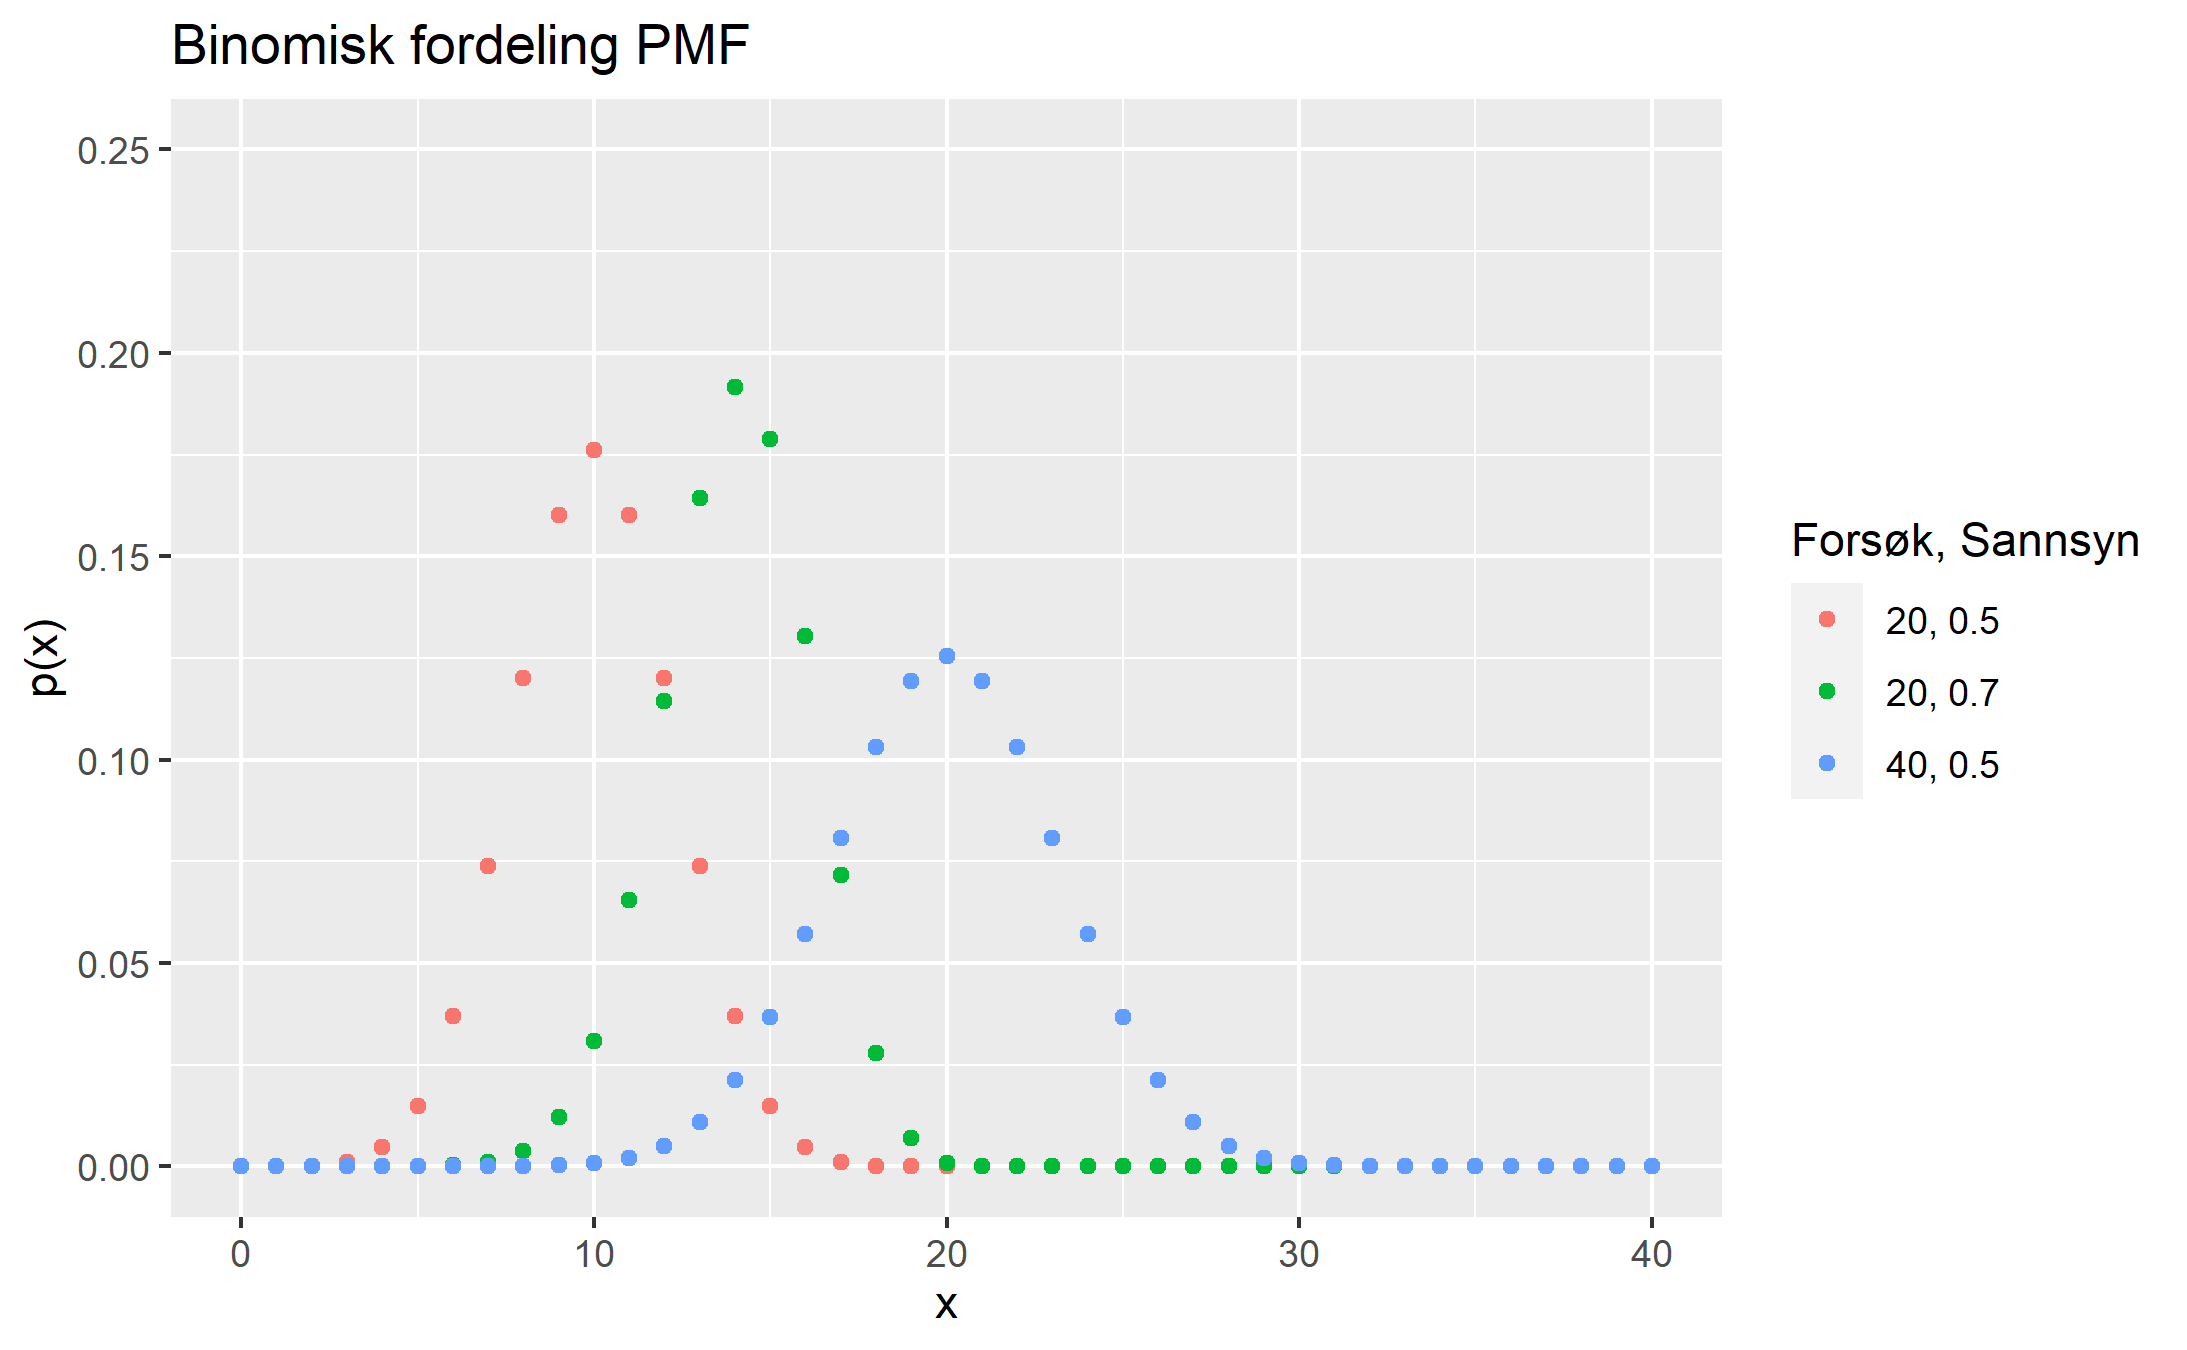
\includegraphics[width=\textwidth]{bilete/binompmf.png}
  \end{minipage}
  \hfill
  \begin{minipage}[b]{0.49\textwidth}
    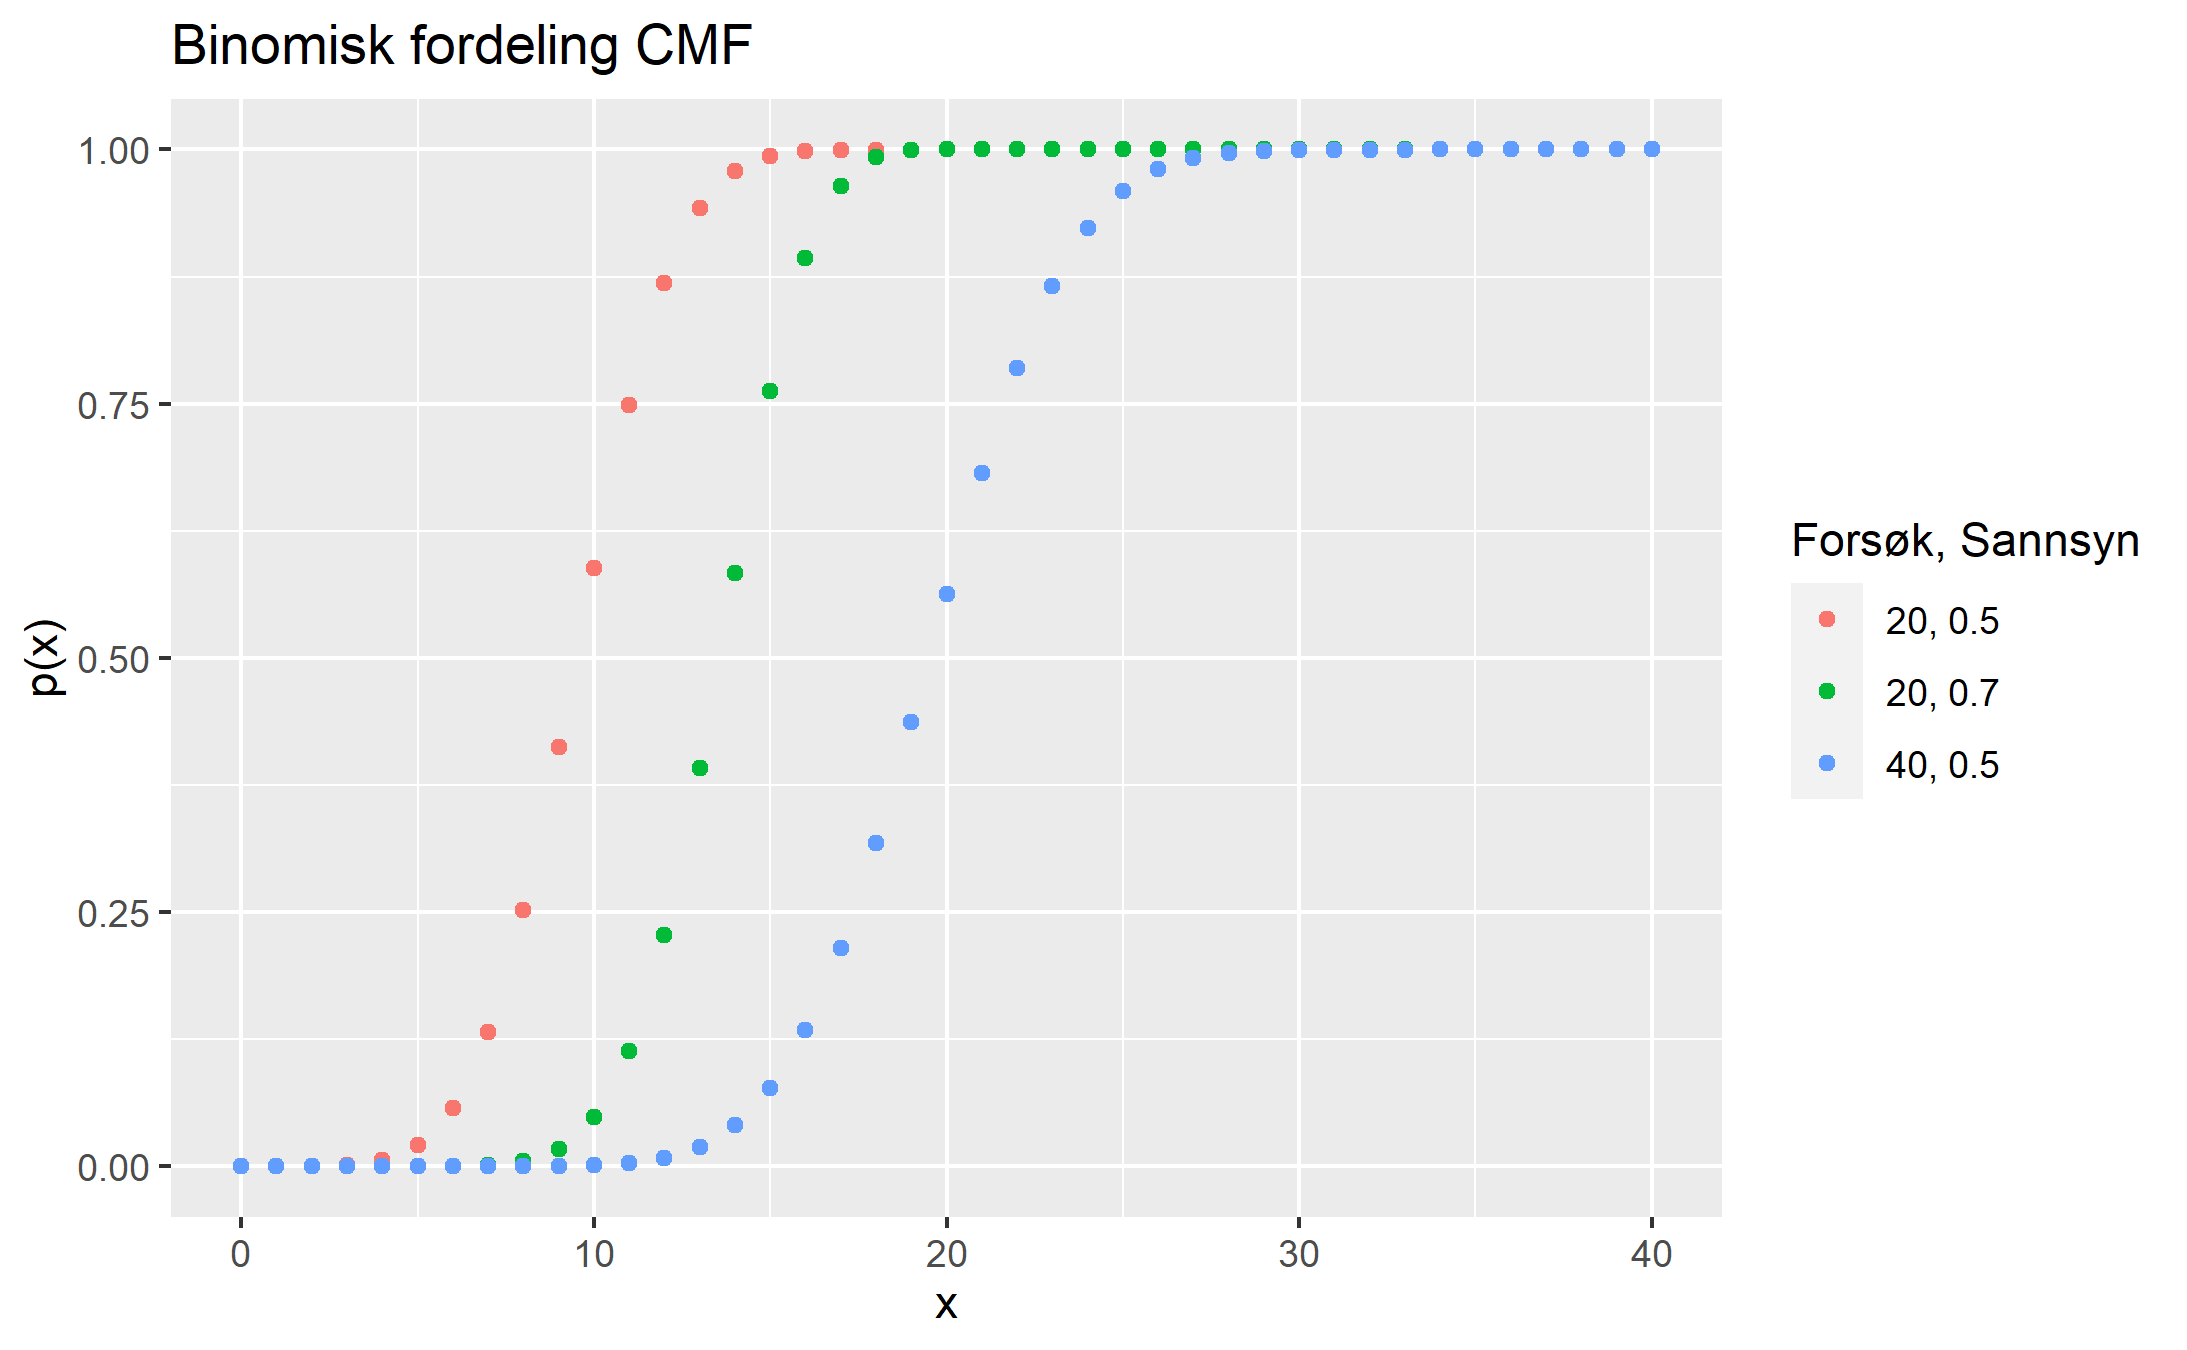
\includegraphics[width=\textwidth]{bilete/binomcdf.png}
  \end{minipage}
\end{figure}

Om $X$ er antalet vellukka hendingar i $n$ bernoulli forsøk er $X$ binomisk fordelt. Den har parameter $p$ for sannsynet for eit vellukka forsøk og $n$ for antal forsøk totalt.

\begin{equation}
    f(x; n, p) = b(x; n, p) = \binom{n}{x}p^x (1-p)^{n-x}
\end{equation}

\begin{equation}
    F(x; n, p) = P(X \leq x) = \sum_{i = 0}^{x} \binom{n}{i}p^i(1-p)^{n-i}
\end{equation}

\begin{equation}
    E[X] = np, \qquad \text{Var}(X) = np(1-p)
\end{equation}

\subsubsection{Bernoulli Prosessen} \label{chap:bernoulli}
For å forstå binomisk fordeling og når denne fordelinga er aktuelle må ein forstå bernoulli prosessen. Under ein streng definisjon, er ein bernoulli prosess ein prosess med følgande eigenskapar:

\begin{enumerate}
    \item Eksperimentet må bestå av gjentatte forsøk.
    \item Kvart forsøk har utfall som er enten vellukka eller mislukka.
    \item Sannsynlegheita for eit vellukka eksperiment $p$ må vere konstant.
    \item Forsøka må vere uavhengige.
\end{enumerate}

\subsection{Negativ-binomisk fordeling}
\begin{figure}[H]
  \centering
  \begin{minipage}[b]{0.49\textwidth}
    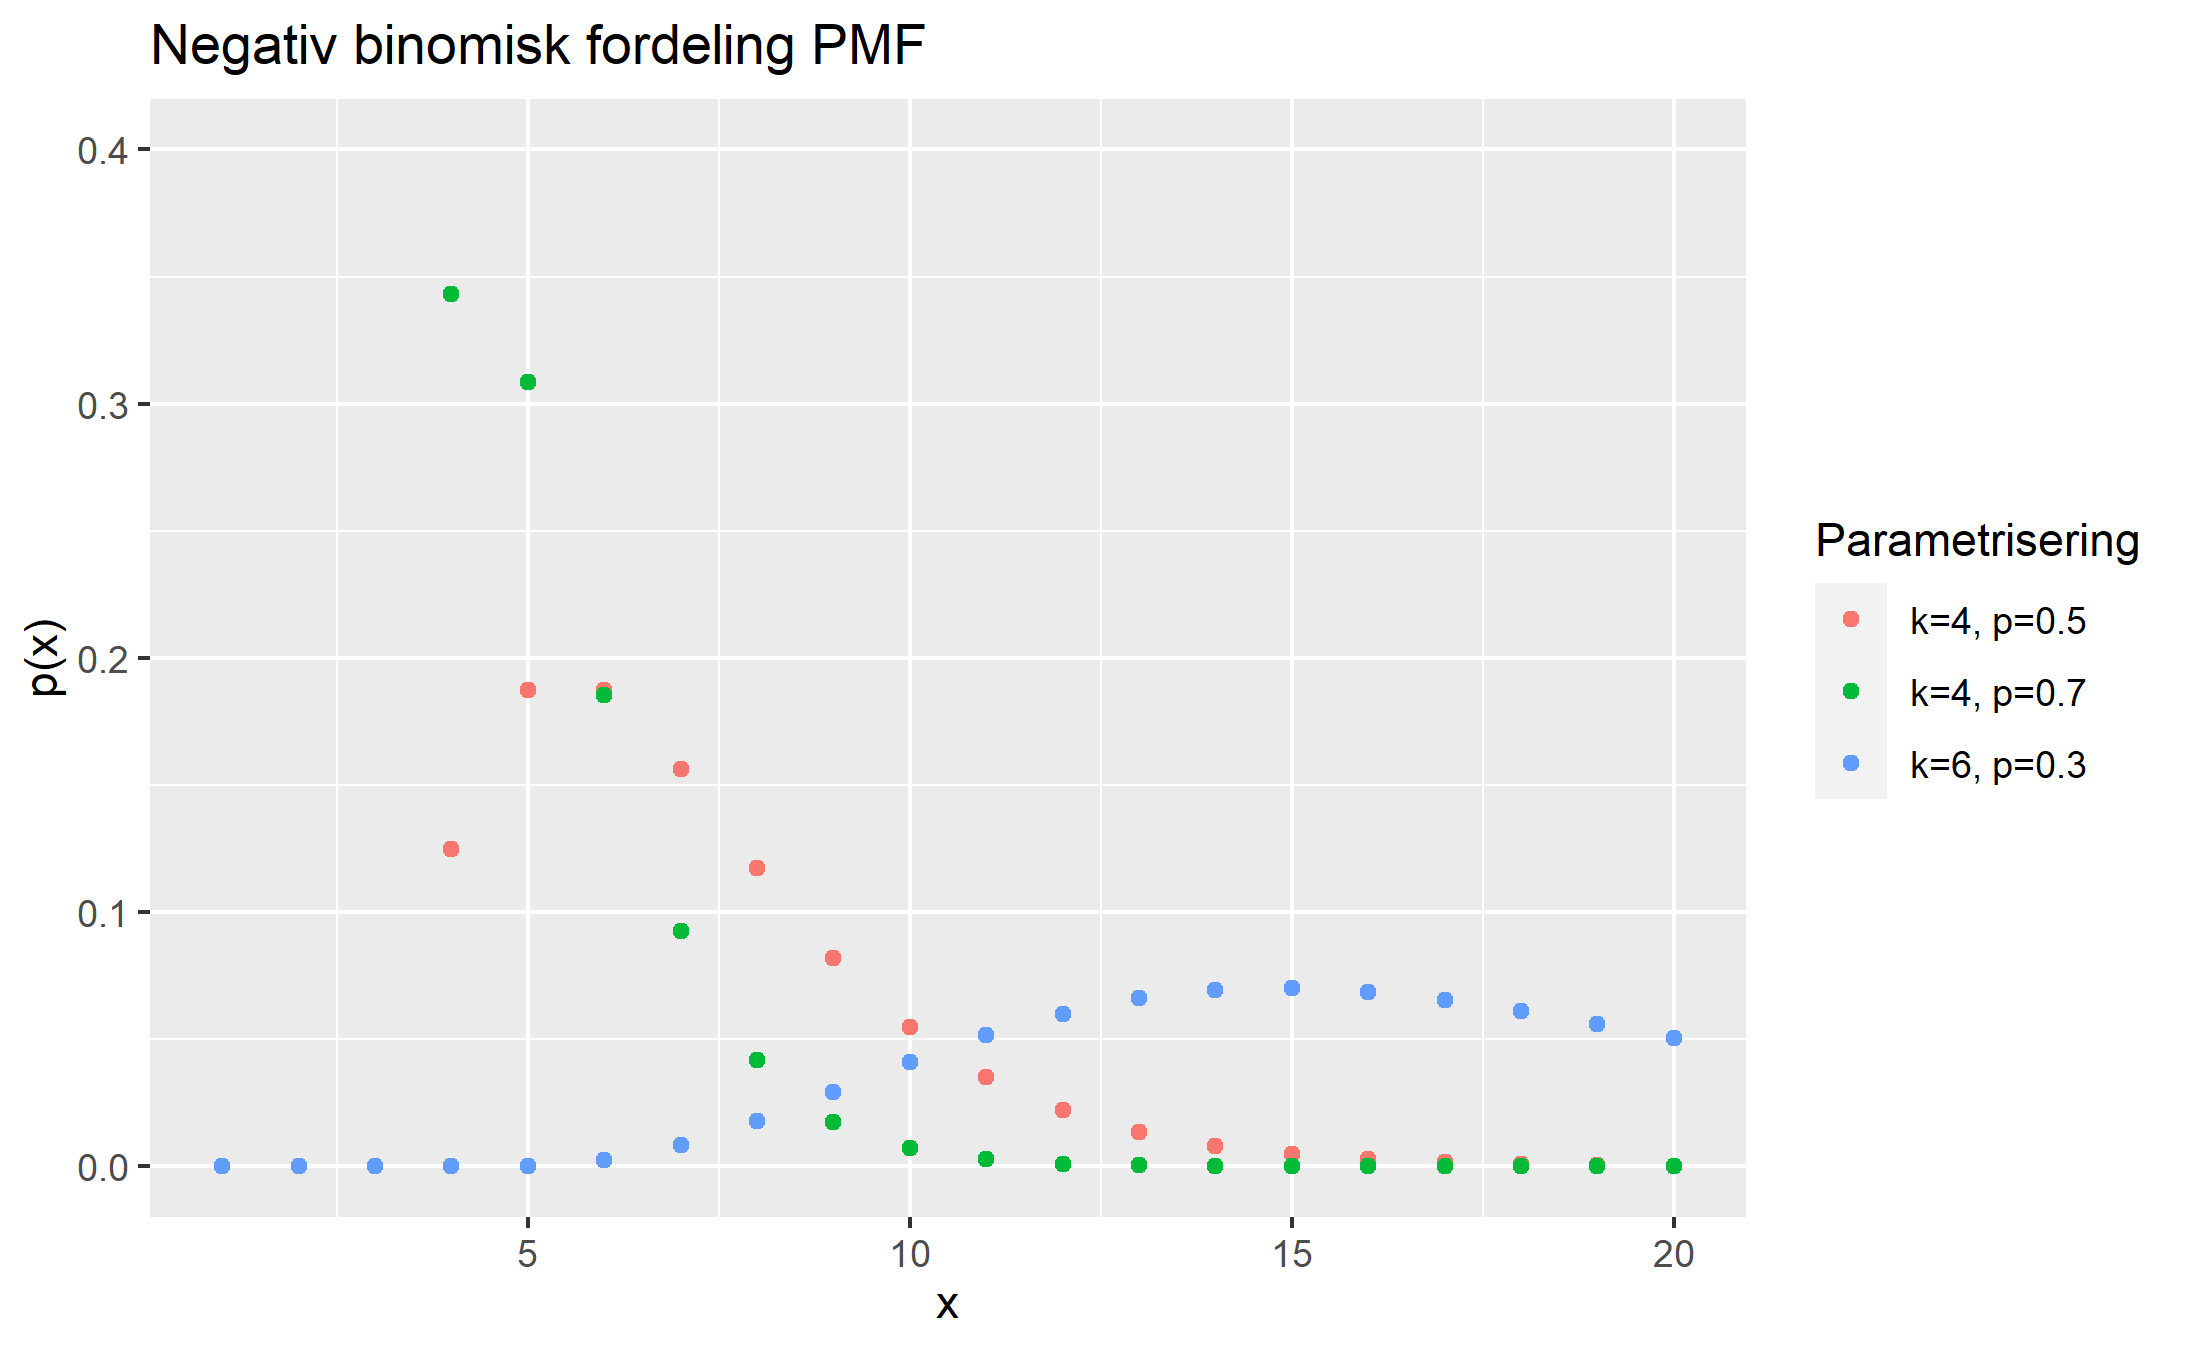
\includegraphics[width=\textwidth]{bilete/negbinpmf.png}
  \end{minipage}
  \hfill
  \begin{minipage}[b]{0.49\textwidth}
    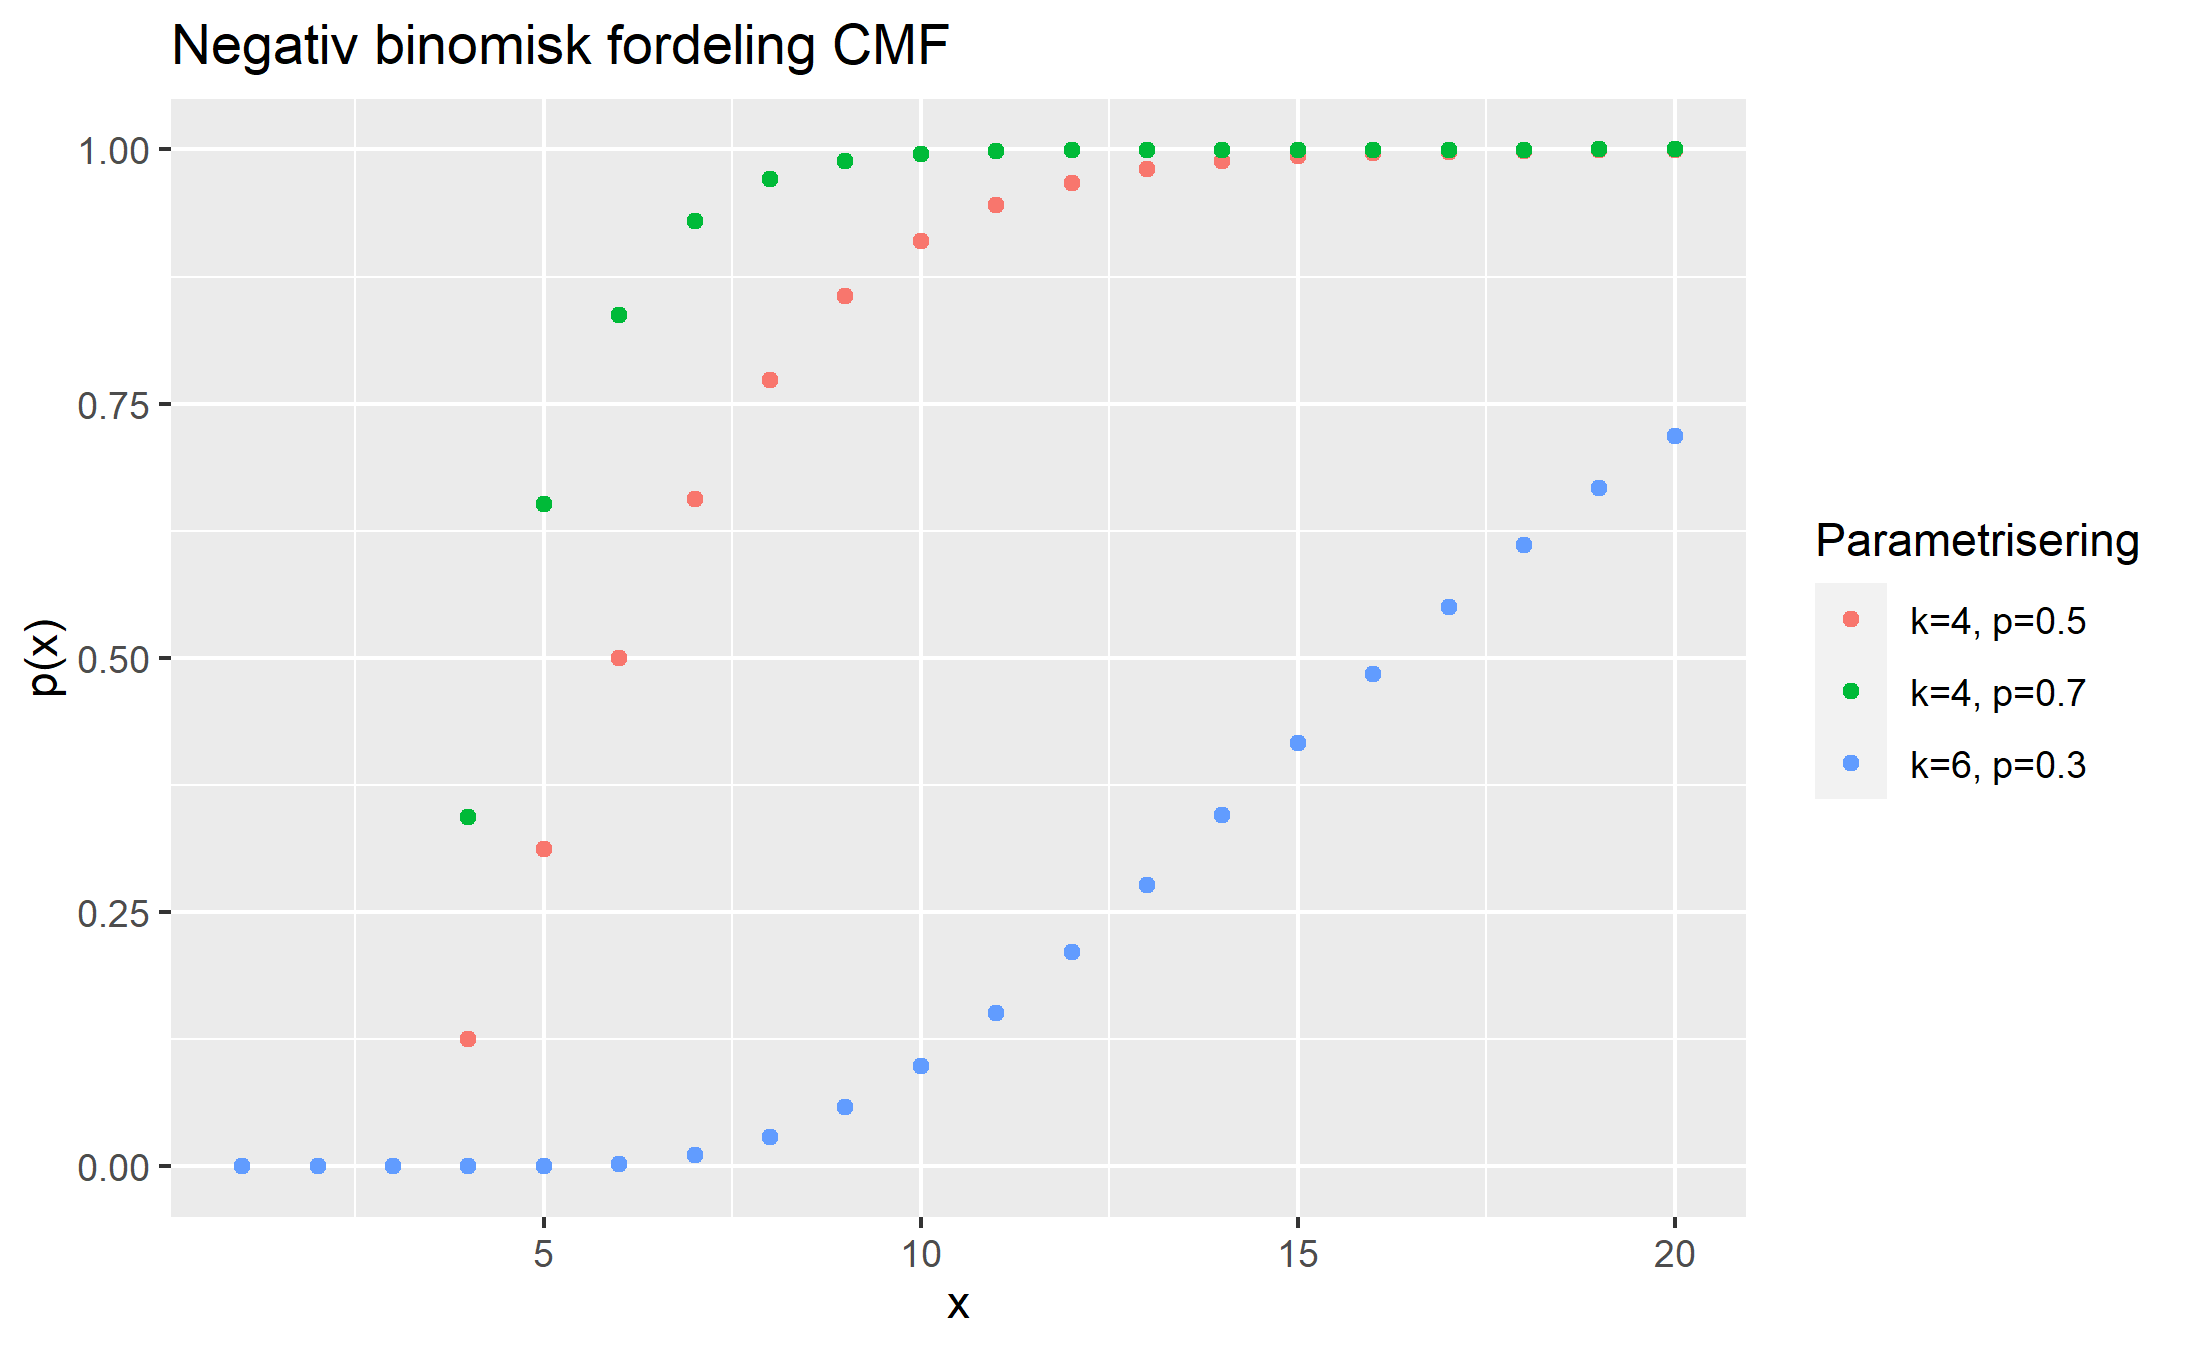
\includegraphics[width=\textwidth]{bilete/negbincdf.png}
  \end{minipage}
\end{figure}
Om eksperimentet følger same eigenskap som bernoulli prosess en \ref{chap:bernoulli}, men istadenfor lar me $X$ = Nummeret på forsøket der suksess $k$ tar stad. Då er $X$ negativ binomisk fordelt. 

\begin{equation}
    f(x; k, p) = b^*(x; k, p) = \binom{x - 1}{k - 1}p^k (1-p)^{x - k}
\end{equation}

\begin{equation}
    F(x; k, p) = P(X \leq x) = \sum_{i = 0}^{x} \binom{i - 1}{k - 1}p^k (1-p)^{i - k}
\end{equation}

\begin{equation}
    E[X] = \frac{k}{p}, \qquad \text{Var}(X) = k\frac{1-p}{p^2}
\end{equation}

\subsubsection{Alternative parametriseringar}
Det er viktig å bemerke seg at det er fleire parametriseringar av negativ-binomisk fordeling. \cite{wiki:negativebinom} Det er 3 variantar av desse. $X$ teller...

\begin{enumerate}
    \item $k$ mislukka gitt $r$ vellukka.
    \item $n$ forsøk gitt $k$ vellukka. (Dette er parametriseringa over)
    \item $r$ vellukka gitt $n$ forsøk. (Dette er binomisk fordeling \ref{chap:binomford})
\end{enumerate}

Dei alternative parametriseringane blir ikkje gått gjennom her, men det er viktigt å vere obs på at desse finst.

\subsection{Multinomisk fordeling}
Ein multinomisk fordeling er ein fleirvariabels parameter og er derfor ikkje plotta som dei andre fordelingane.

\begin{equation}
    f(x:1, \dots, x_k; p_1, \dots, p_k, n) = \frac{n!}{x_1! \dots x_k!}p_1^{x_1}\dots p_k^{x_k}
\end{equation}

\begin{equation}
    E[X_i] = np_i, \qquad \text{Var}(X_i) = np_i(1-p_i), \qquad \text{Cov}(X_i, X_j) = -np_ip_j
\end{equation}

\subsubsection{Multinomisk eksperiment}
Eit binomisk eksperiment (sjå \ref{chap:bernoulli}) blir eit multinomisk eksperiment om me lar forsøka he fleire utfall. Dei andre eigenskapane er dei same.

\subsection{Geometrisk fordeling}
\begin{figure}[H]
  \centering
  \begin{minipage}[b]{0.49\textwidth}
    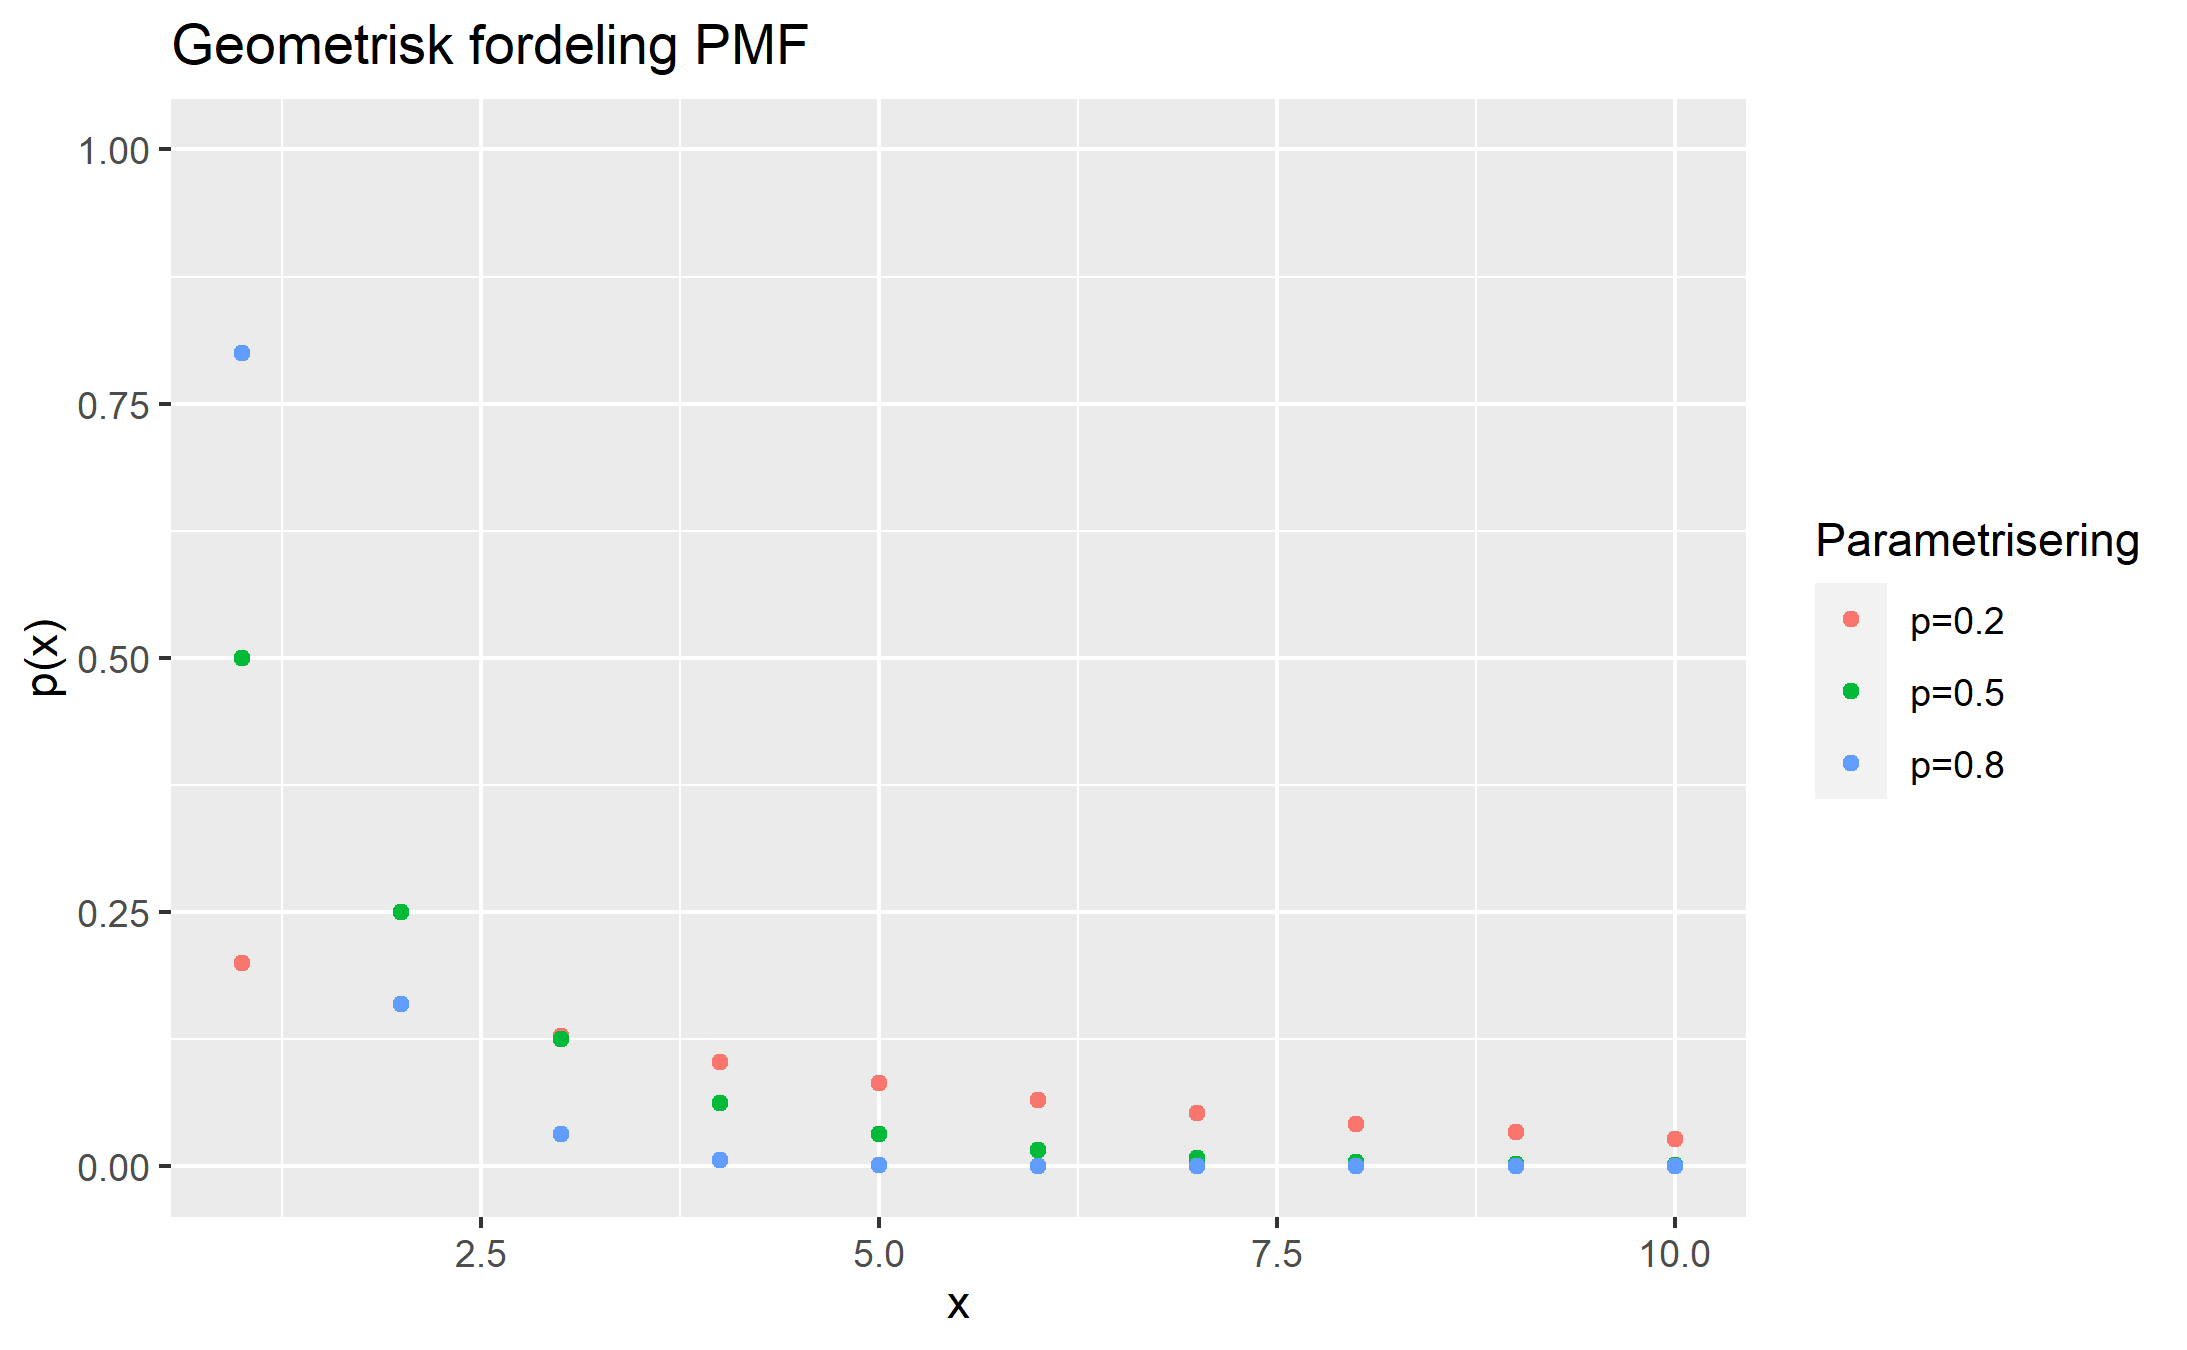
\includegraphics[width=\textwidth]{bilete/geompmf.png}
  \end{minipage}
  \hfill
  \begin{minipage}[b]{0.49\textwidth}
    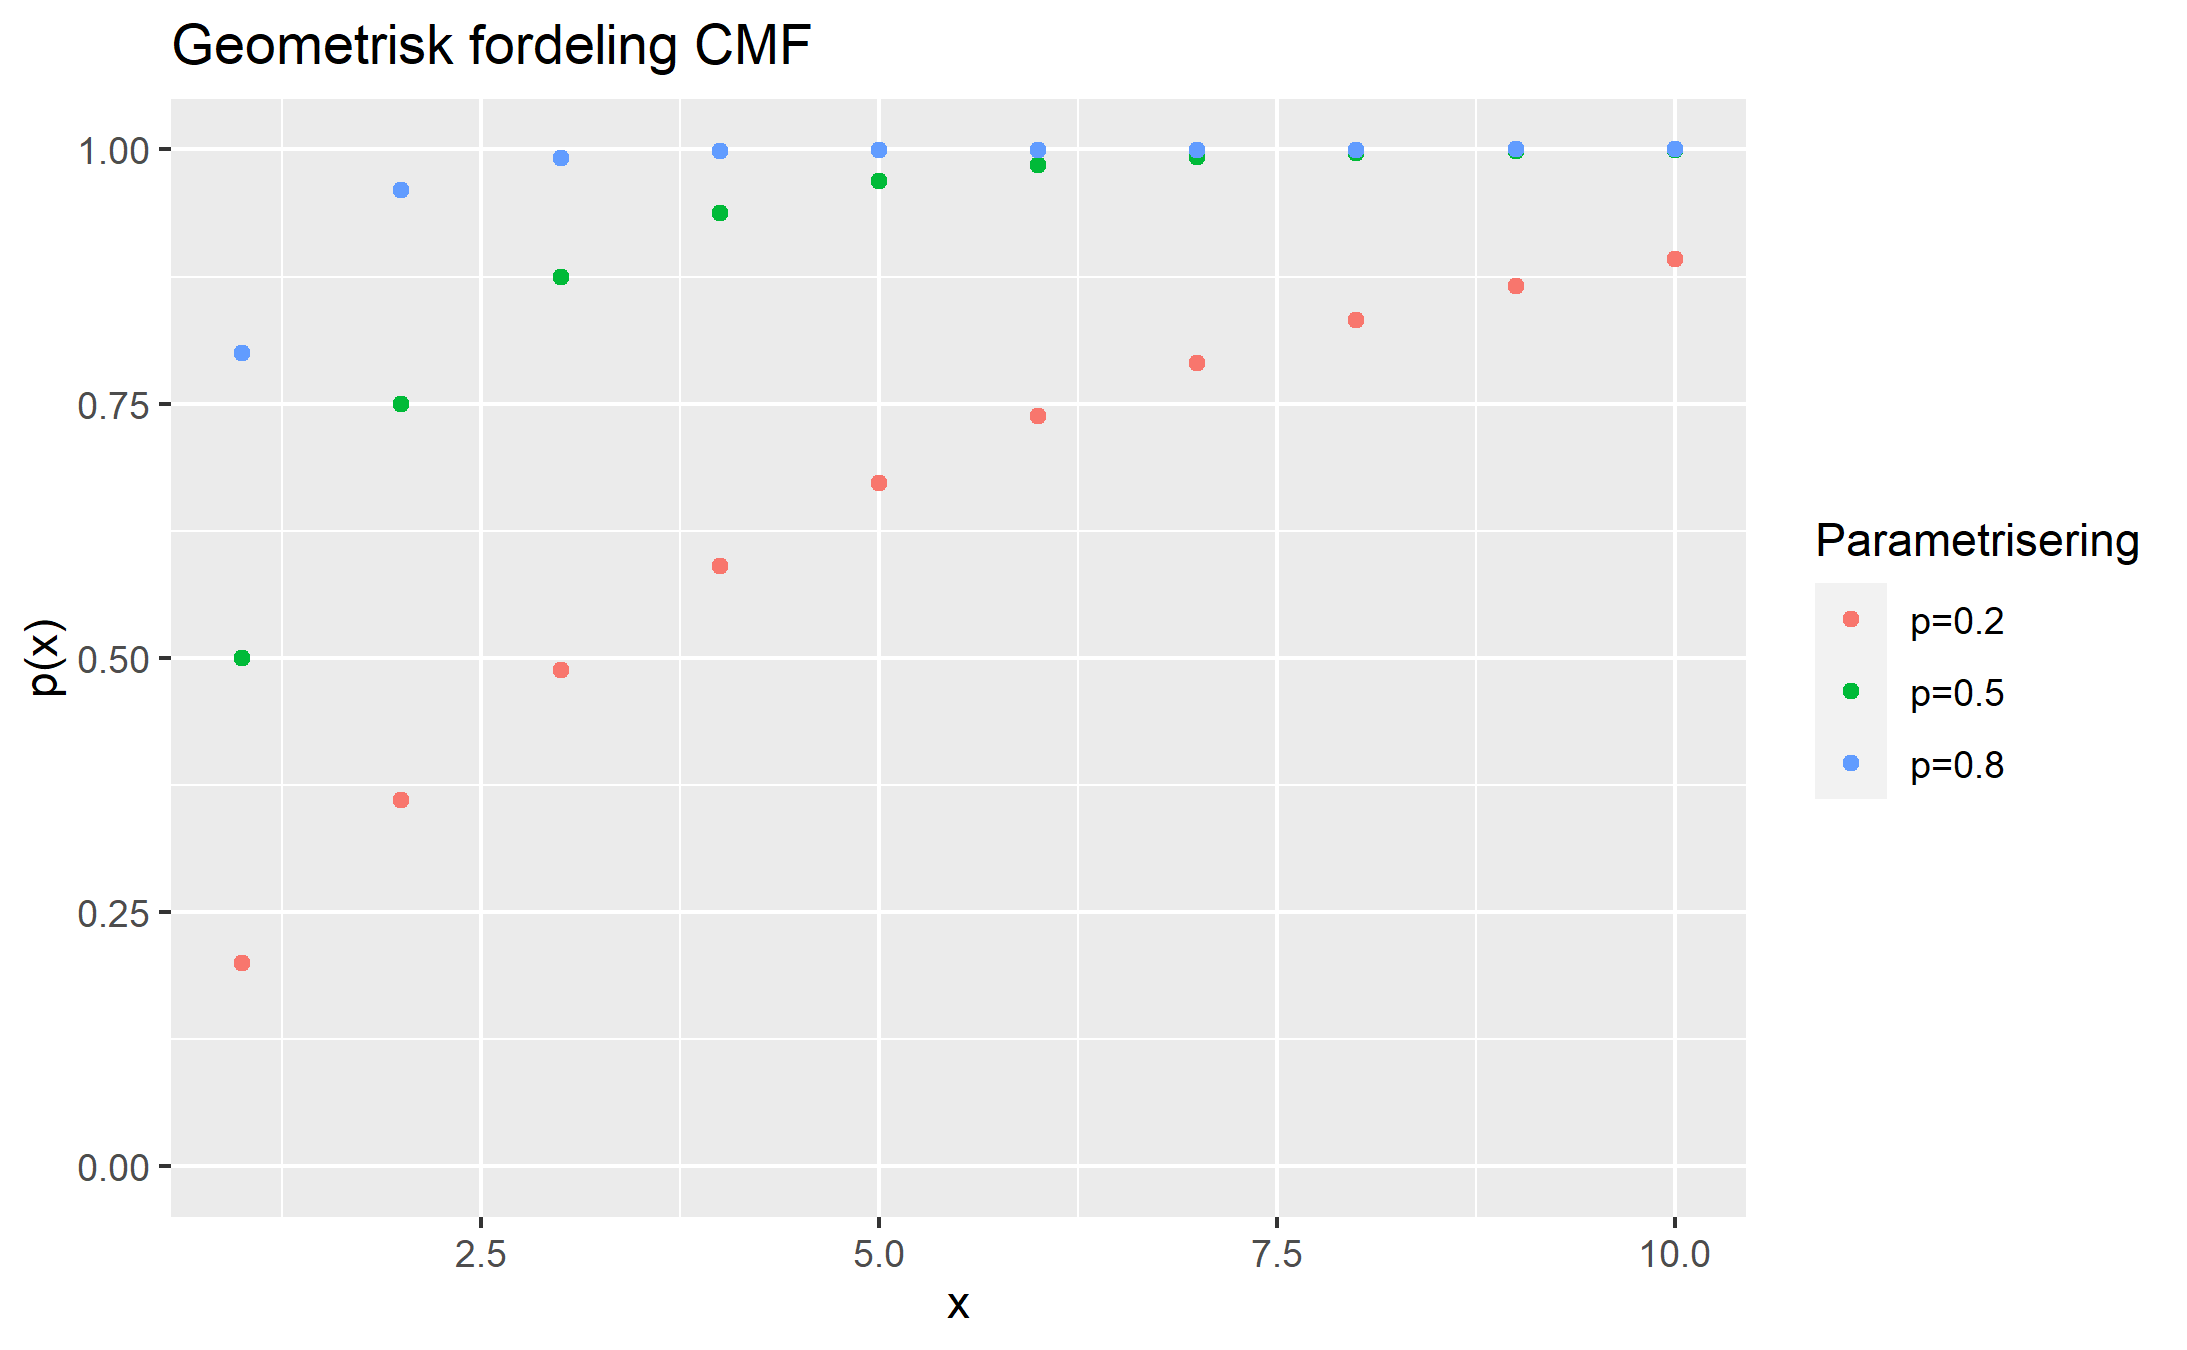
\includegraphics[width=\textwidth]{bilete/geomcdf.png}
  \end{minipage}
\end{figure}

Eit spesialtilfelle av negativ-binomisk fordeling er geometrisk fordeling. Gitt at vi har ein bernoulli prosess \ref{chap:bernoulli}, om $X =$ Antal forsøk inntil 1 suksess, så er $X$ geometrisk fordelt.

\begin{equation}
    f(x; \lambda t) = g(x; 1, p) = (1-p)^{x-1}p, \qquad x = 0, 1, 2, \dots
\end{equation}

\begin{equation}
    F(x; 1, p) = P(X \leq x) = 1 - (1 - p)^x
\end{equation}

\begin{equation}
    E[X] = \frac{1}{p}, \qquad \text{Var}(X) = \frac{1-p}{p^2}
\end{equation}

\subsection{Poissonfordeling}
\begin{figure}[H]
  \centering
  \begin{minipage}[b]{0.49\textwidth}
    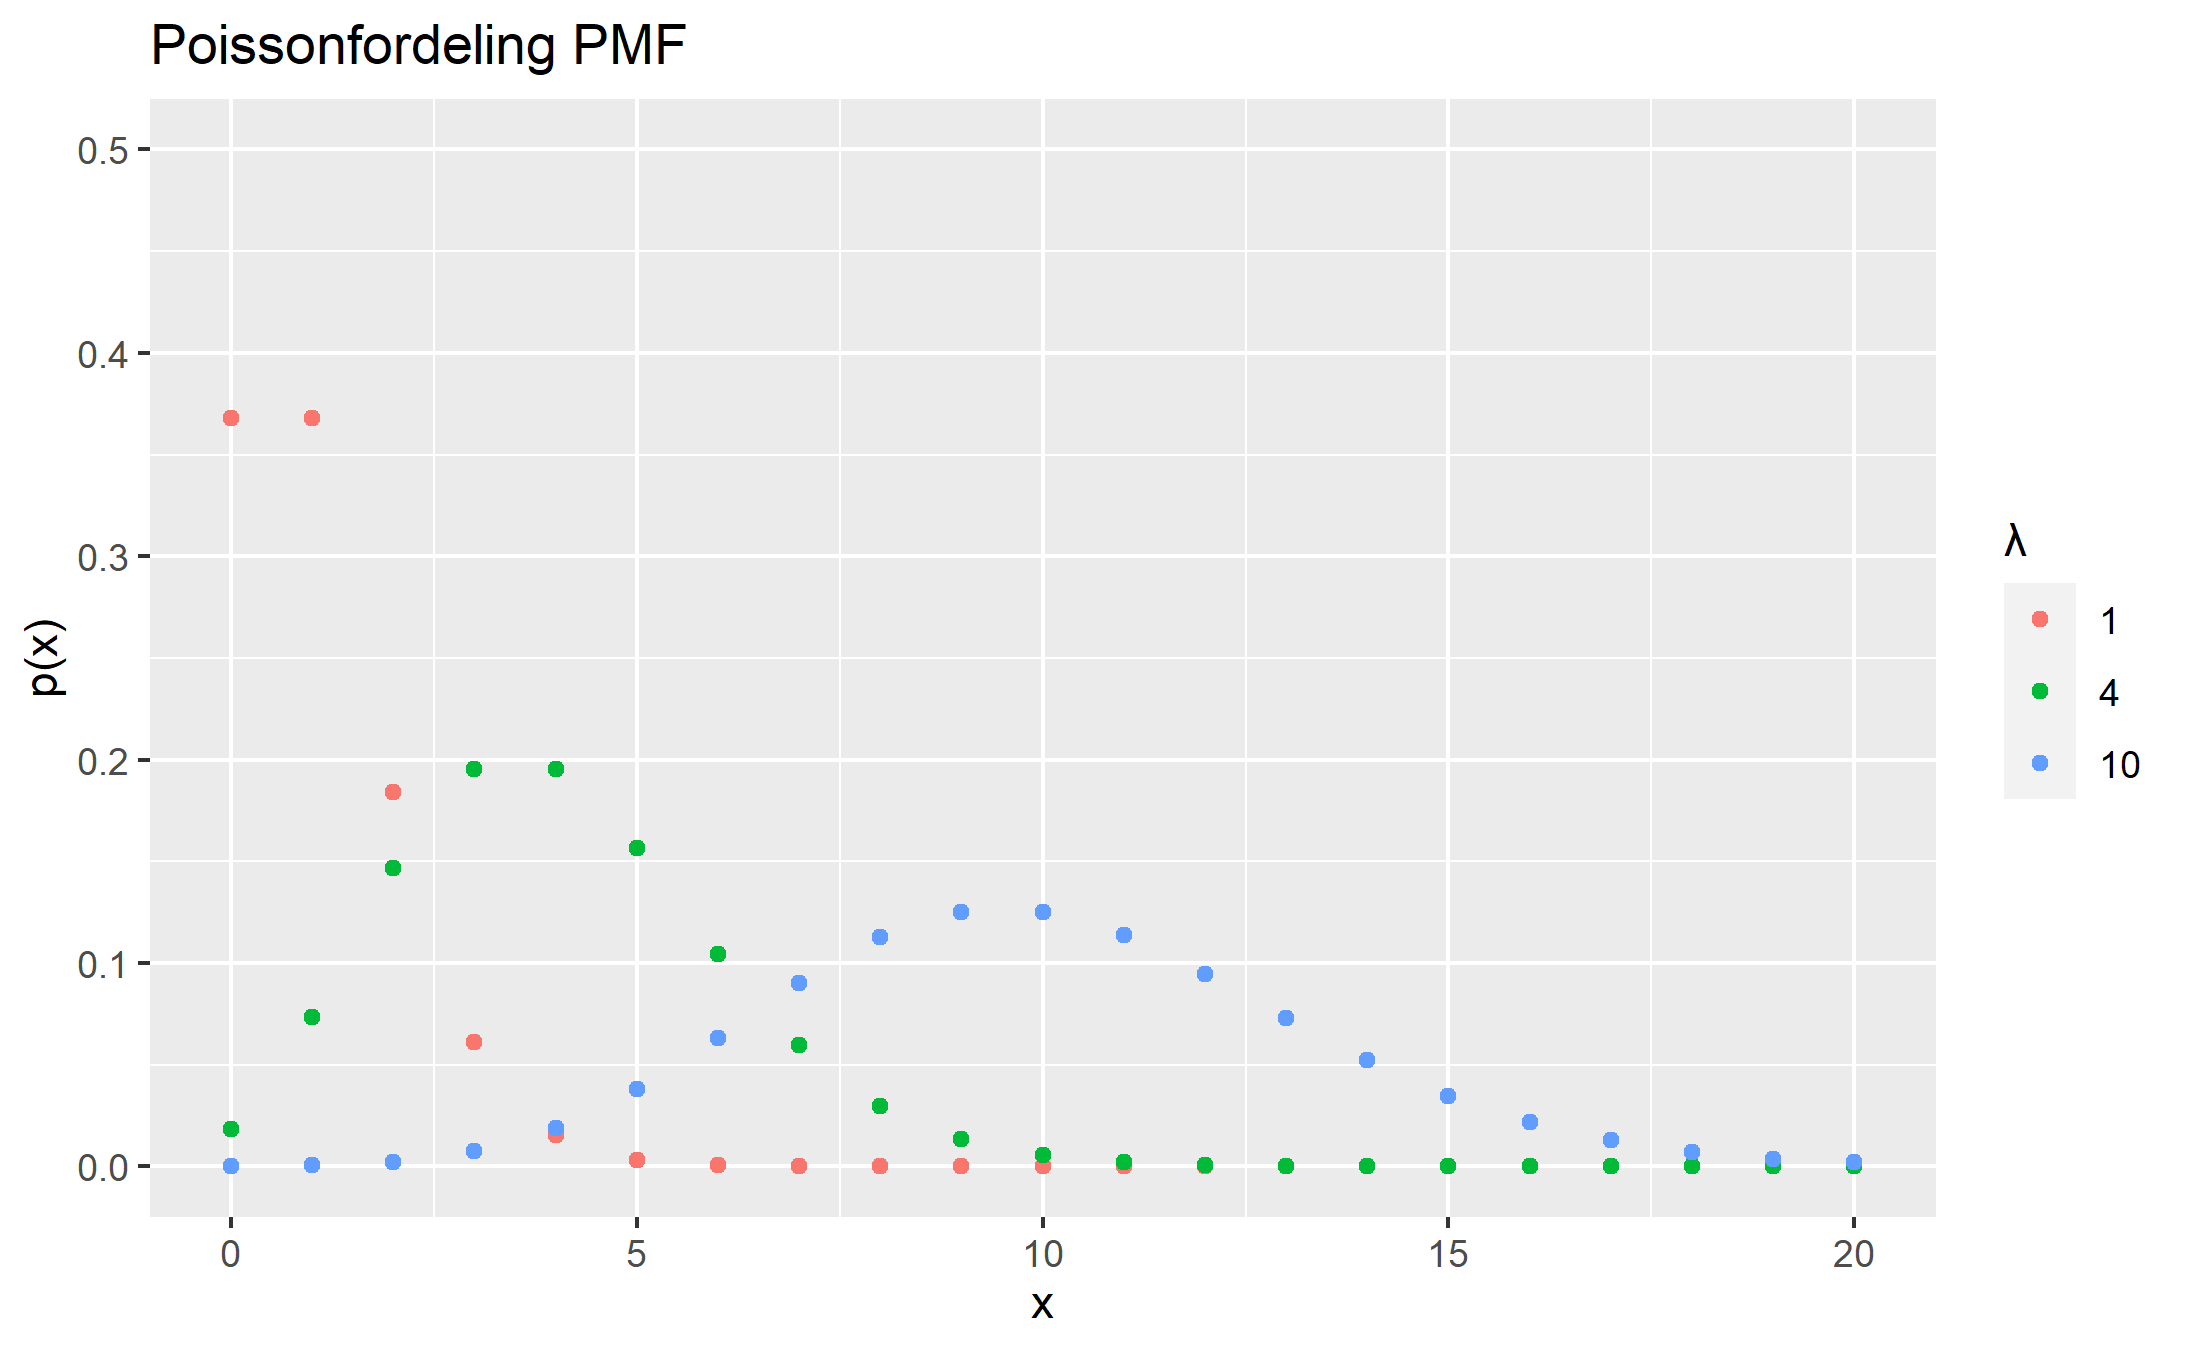
\includegraphics[width=\textwidth]{bilete/poispmf.png}
  \end{minipage}
  \hfill
  \begin{minipage}[b]{0.49\textwidth}
    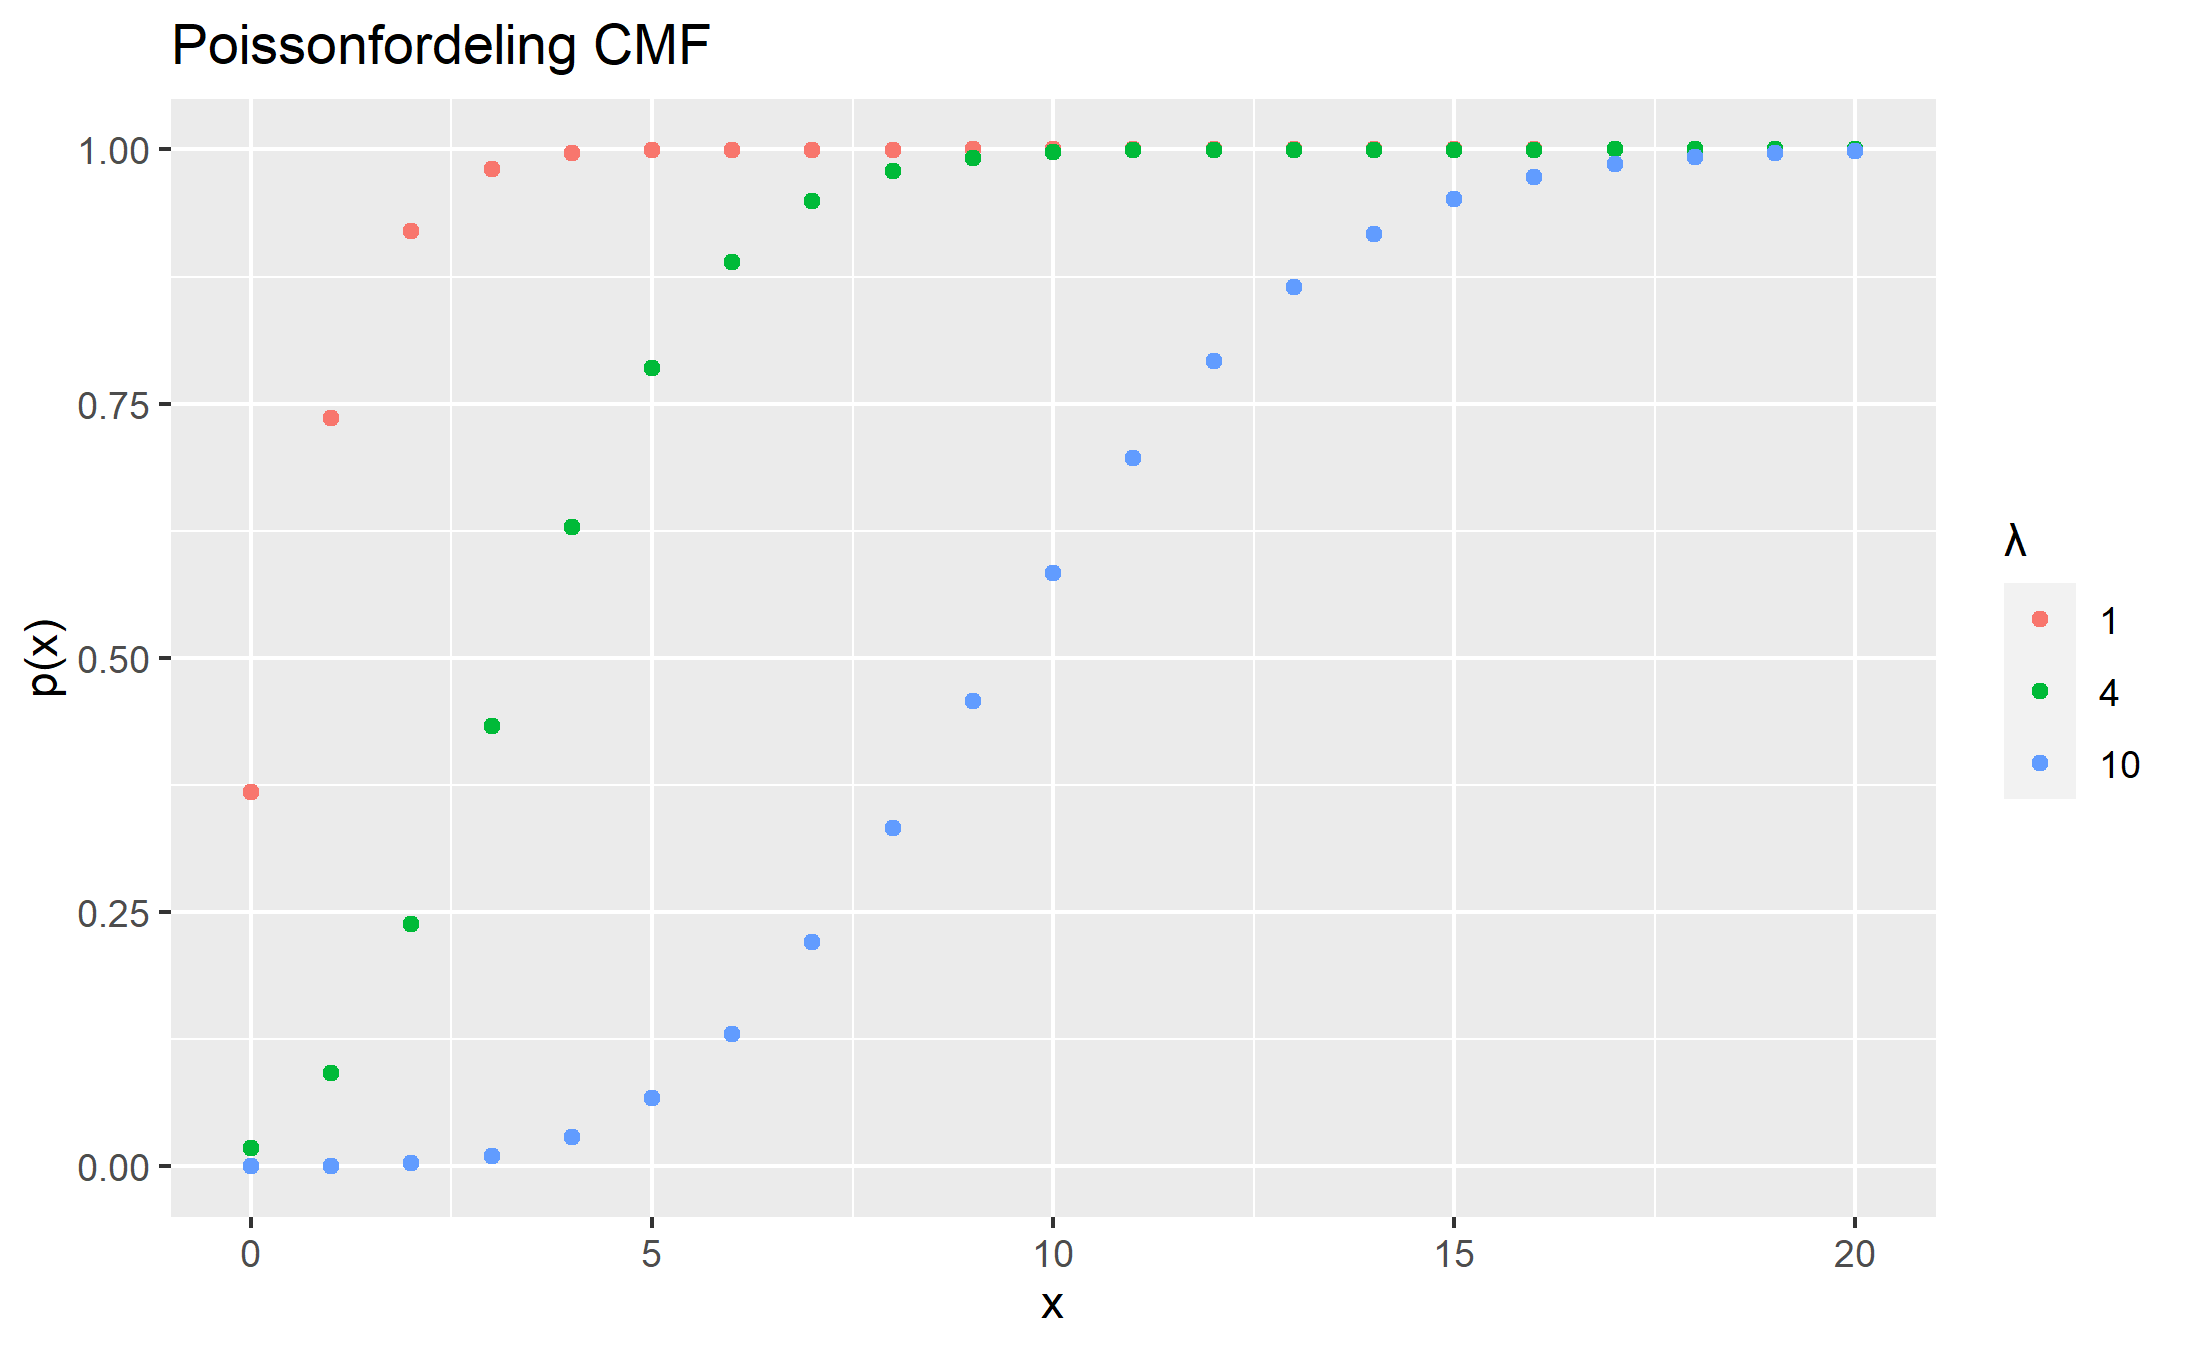
\includegraphics[width=\textwidth]{bilete/poiscdf.png}
  \end{minipage}
\end{figure}

Poissonfordelinga beskriver sannsynet for antalet hendingar som skjer i eit avgrensa plass og/eller tidsrom der hendingane er uavhengige frå kvarandre (Les her for meir om poisson prosessen: \ref{chap:poissonpro}). 

\begin{equation}
    f(x; \lambda t) = p(x; \lambda t) = \frac{e^{-\lambda t}(\lambda t)^x}{x!}, \qquad x = 0, 1, 2, \dots
\end{equation}

\begin{equation}
    F(x; \lambda t) = P(X \leq x) = \sum_{i = 0}^{x} \frac{e^{-\lambda t}(\lambda t)^i}{i!}
\end{equation}

\begin{equation}
    E[X] = \lambda t, \qquad \text{Var}(X) = \lambda t
\end{equation}

\subsubsection{Poisson prosessen}\label{chap:poissonpro}
Ein stokastisk variabel $X$ er poissonfordelt når $X$ er antalet hendingar i ein poisson prosess. Poisson prosessen har følgande eigenskapar:

\begin{enumerate}
    \item Antalet hendingar i eit tidsintervall eller område er uavhengig antalet hendingar i eit anna, disjunkt tidsintervall eller område. Dette gjer at poisson prosessen er \textit{minnelaus }\ref{memless}.
    \item Sannsynet for eit enkelt utfall i eit lite tidsrom eller område er proporsjonalt med størelsen på intervallet eller området og er uavhengig antalet hendingar utanfor dette tidsrommet eller området.
    \item Sannsynet for at meir enn ein hending vil skje i eit tidsintervall er neglisjerbart.
\end{enumerate}

\subsection{Hypergeometrisk fordeling}
\begin{figure}[H]
  \centering
  \begin{minipage}[b]{0.49\textwidth}
    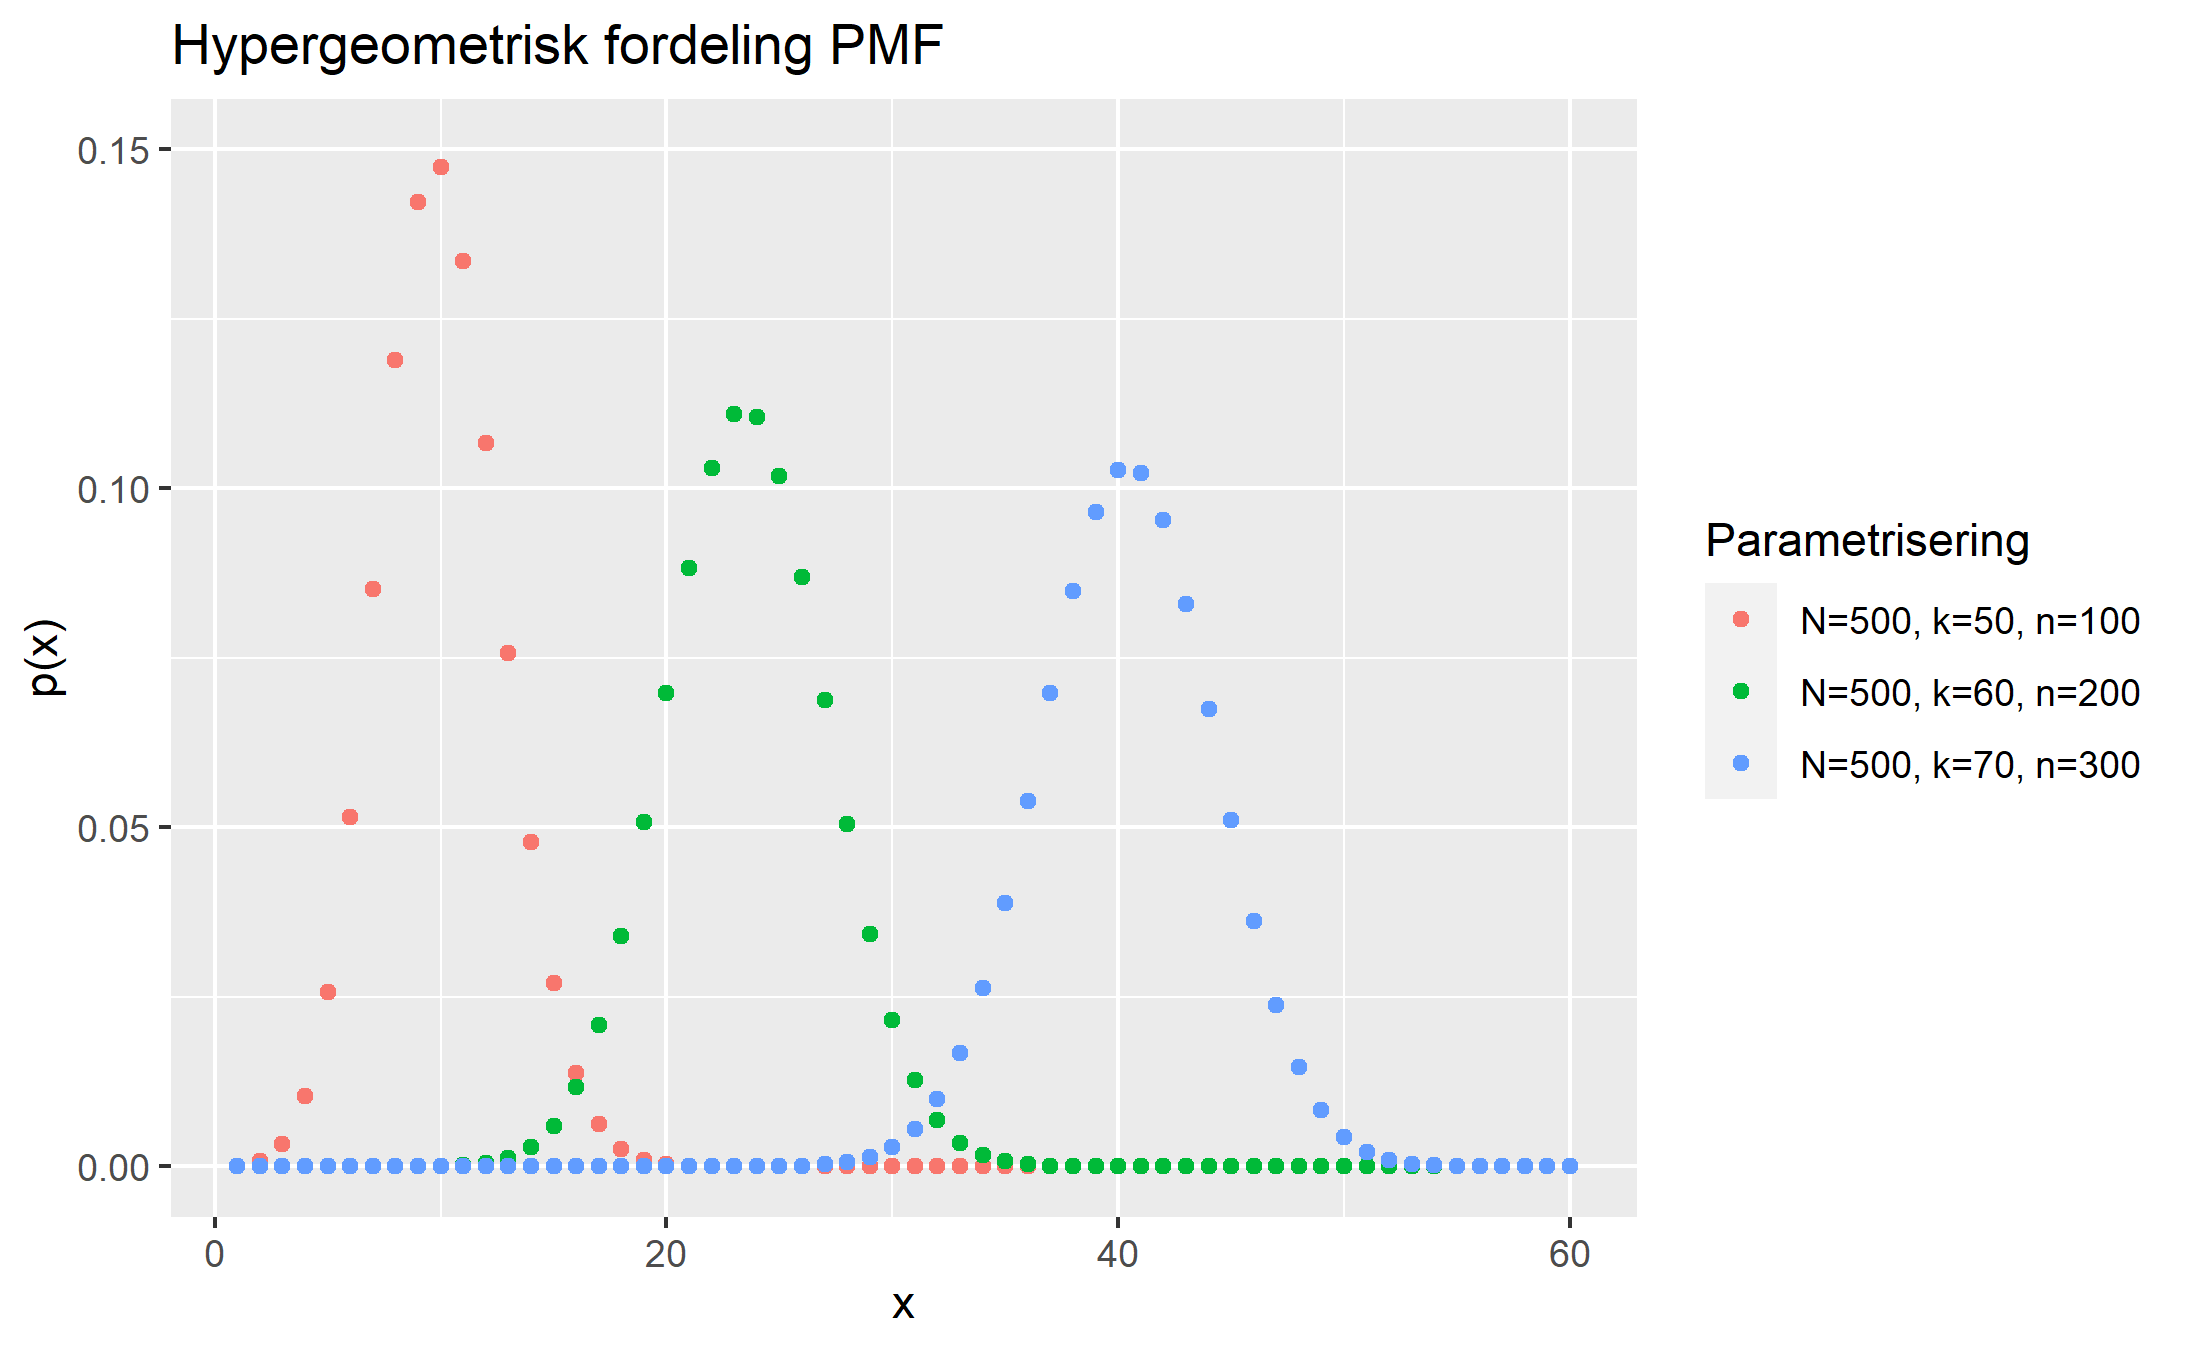
\includegraphics[width=\textwidth]{bilete/hypergeompmf.png}
  \end{minipage}
  \hfill
  \begin{minipage}[b]{0.49\textwidth}
    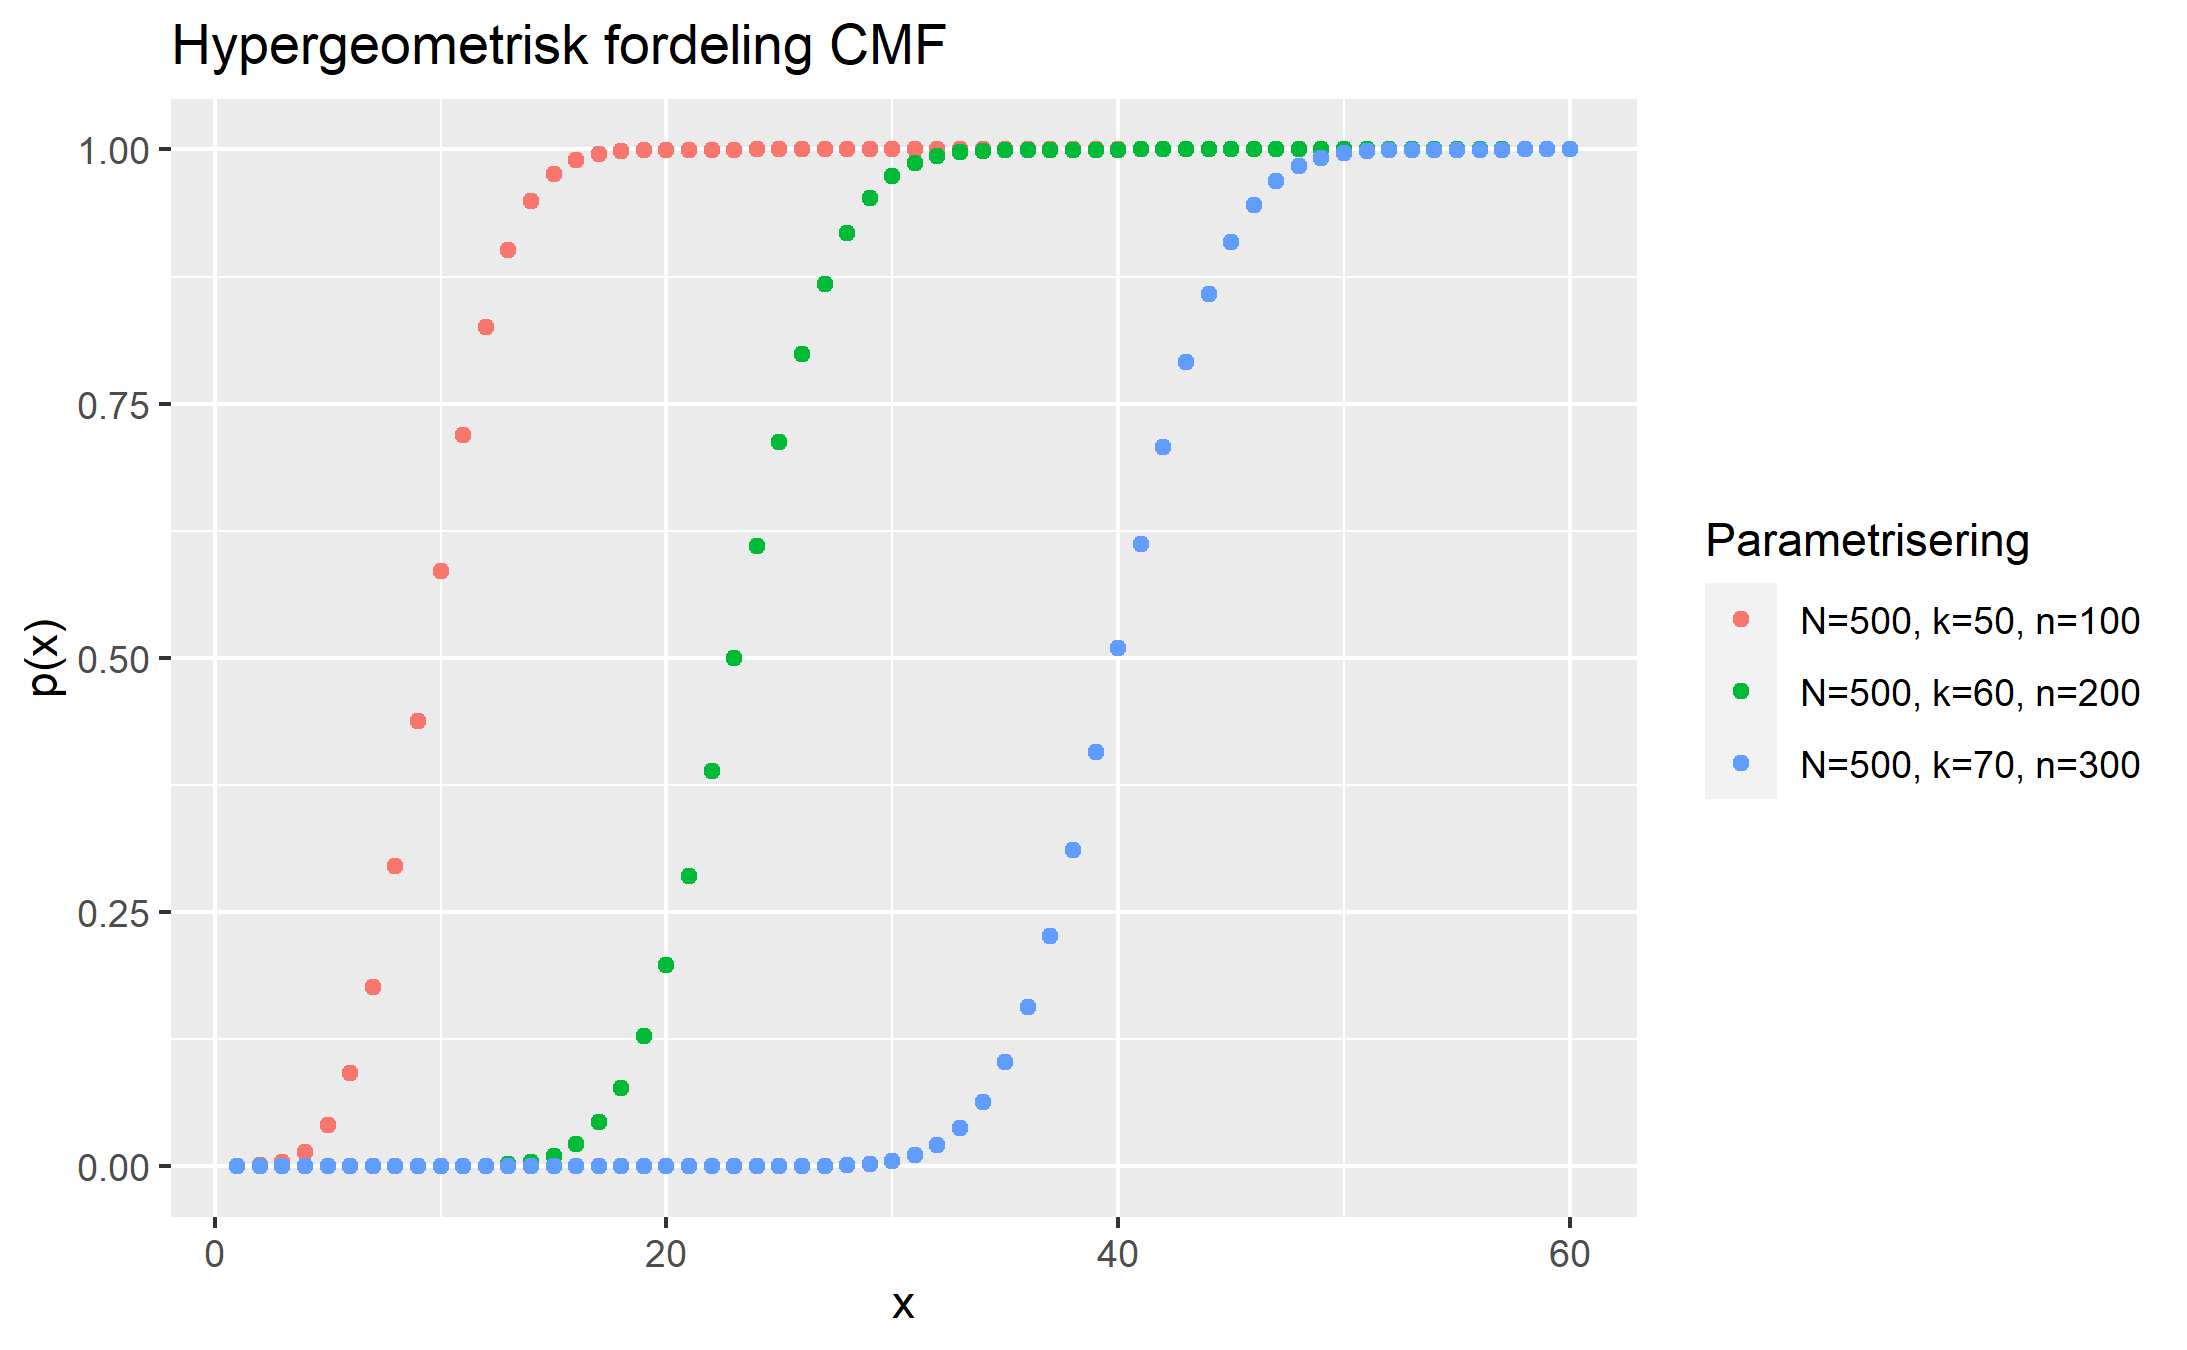
\includegraphics[width=\textwidth]{bilete/hypergeomcmf.png}
  \end{minipage}
\end{figure}

Når $X$ er antal vellukka forsøk i eit hypergeometrisk eksperiment (sjå: \ref{chap:hypergeom}) så er den stokastiske variabelen $X$ hypergeometrisk fordelt. Me har parametra $N$ for populasjonsstørelsen, $n$ for antal forsøk og $k$ for antal vellukka/ønska element i populasjonen.

\begin{equation}
    f(x; N, n, k) = h(x; N, n, k) = \frac{\binom{k}{x}\binom{N-k}{n-k}}{\binom{N}{n}},
    \qquad \max\{0, n - (N - k)\} \leq x \leq \min \{n, k\}
\end{equation}

\begin{equation}
    F(x; N, n, k) = P(X \leq x) = \sum_{i = 0}^{x} \frac{\binom{k}{i}\binom{N-k}{n-k}}{\binom{N}{n}}
\end{equation}

\begin{equation}
    E[X] = n\frac{nk}{N}, \qquad \text{Var}(X) = \frac{N-n}{N-1}\cdot n \cdot \frac{k}{N}\left( 1 - \frac{k}{N}\right)
\end{equation}

\subsubsection{Hypergeometrisk eksperiment}\label{chap:hypergeom}
For å ha eit hypergeometrisk eksperiment må eksperimentet ha følgande eigenskapar

\begin{enumerate}
    \item Eit tilfeldig utvalg på størrelse $n$ er valg uten tilbakelegging frå $N$ moglege.
    \item Av $N$ moglege valg er $k$ rekna som vellukka og $N - k$ rekna som mislukka.
\end{enumerate}

Eit hypergeometrisk eksperiment kan derfor minne om eit binomisk, men eit hypergeometrisk eksperiment har eit sannsyn for eit vellukka forsøk $p$ som ikkje er konstant.

\subsection{Diskret uniform fordeling}
\begin{figure}[H]
  \centering
  \begin{minipage}[b]{0.49\textwidth}
    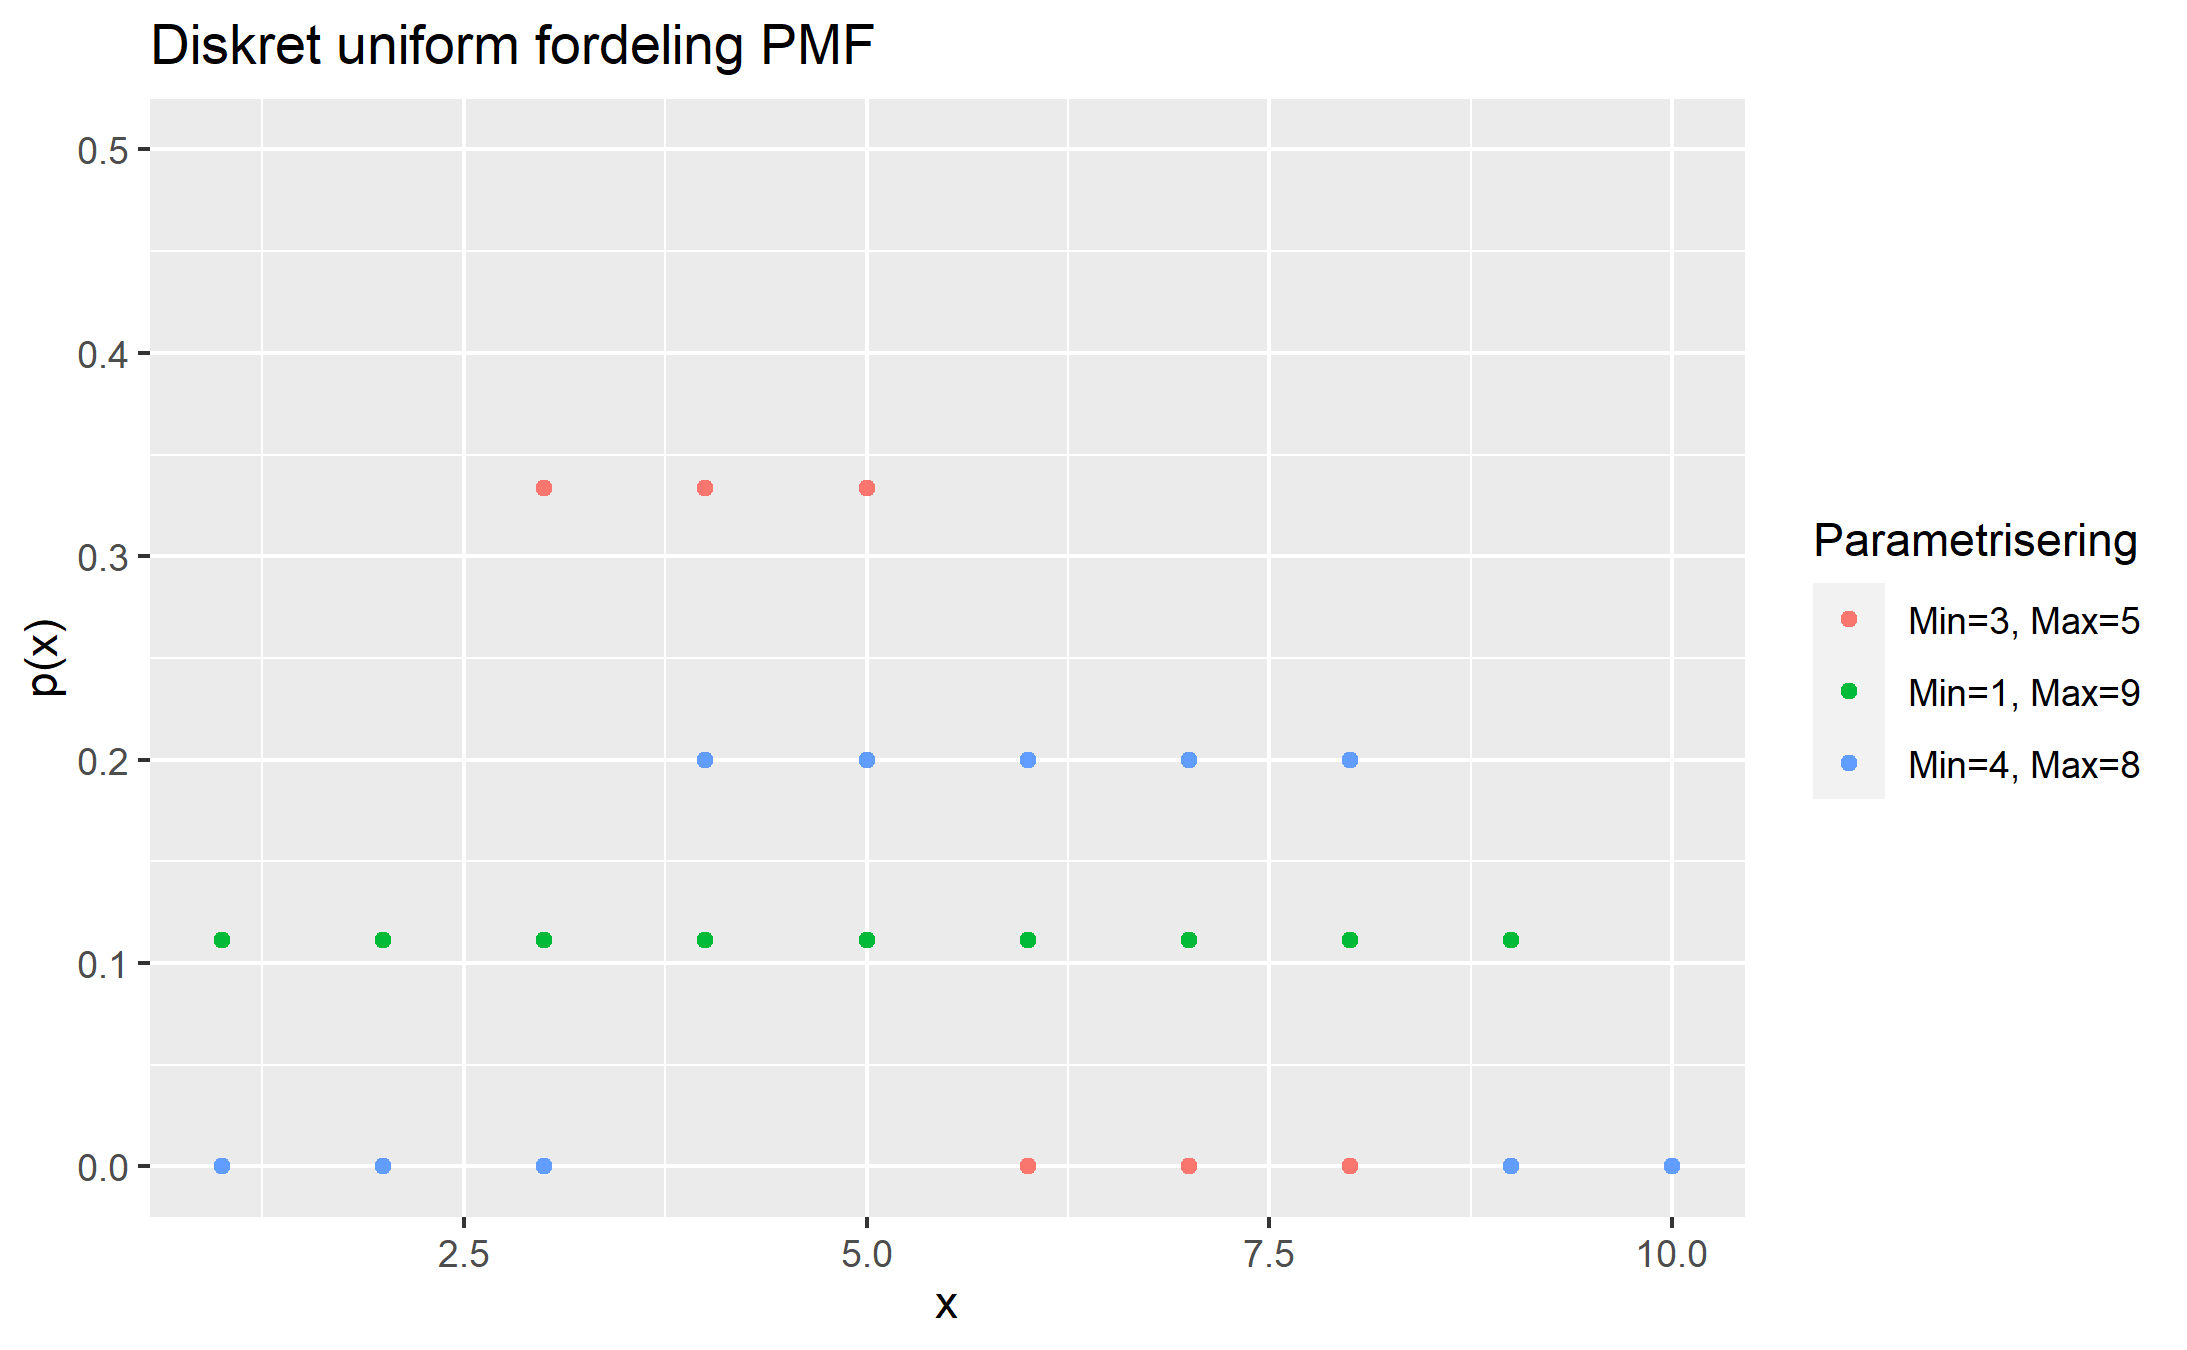
\includegraphics[width=\textwidth]{bilete/diskretuniformpmf.png}
  \end{minipage}
  \hfill
  \begin{minipage}[b]{0.49\textwidth}
    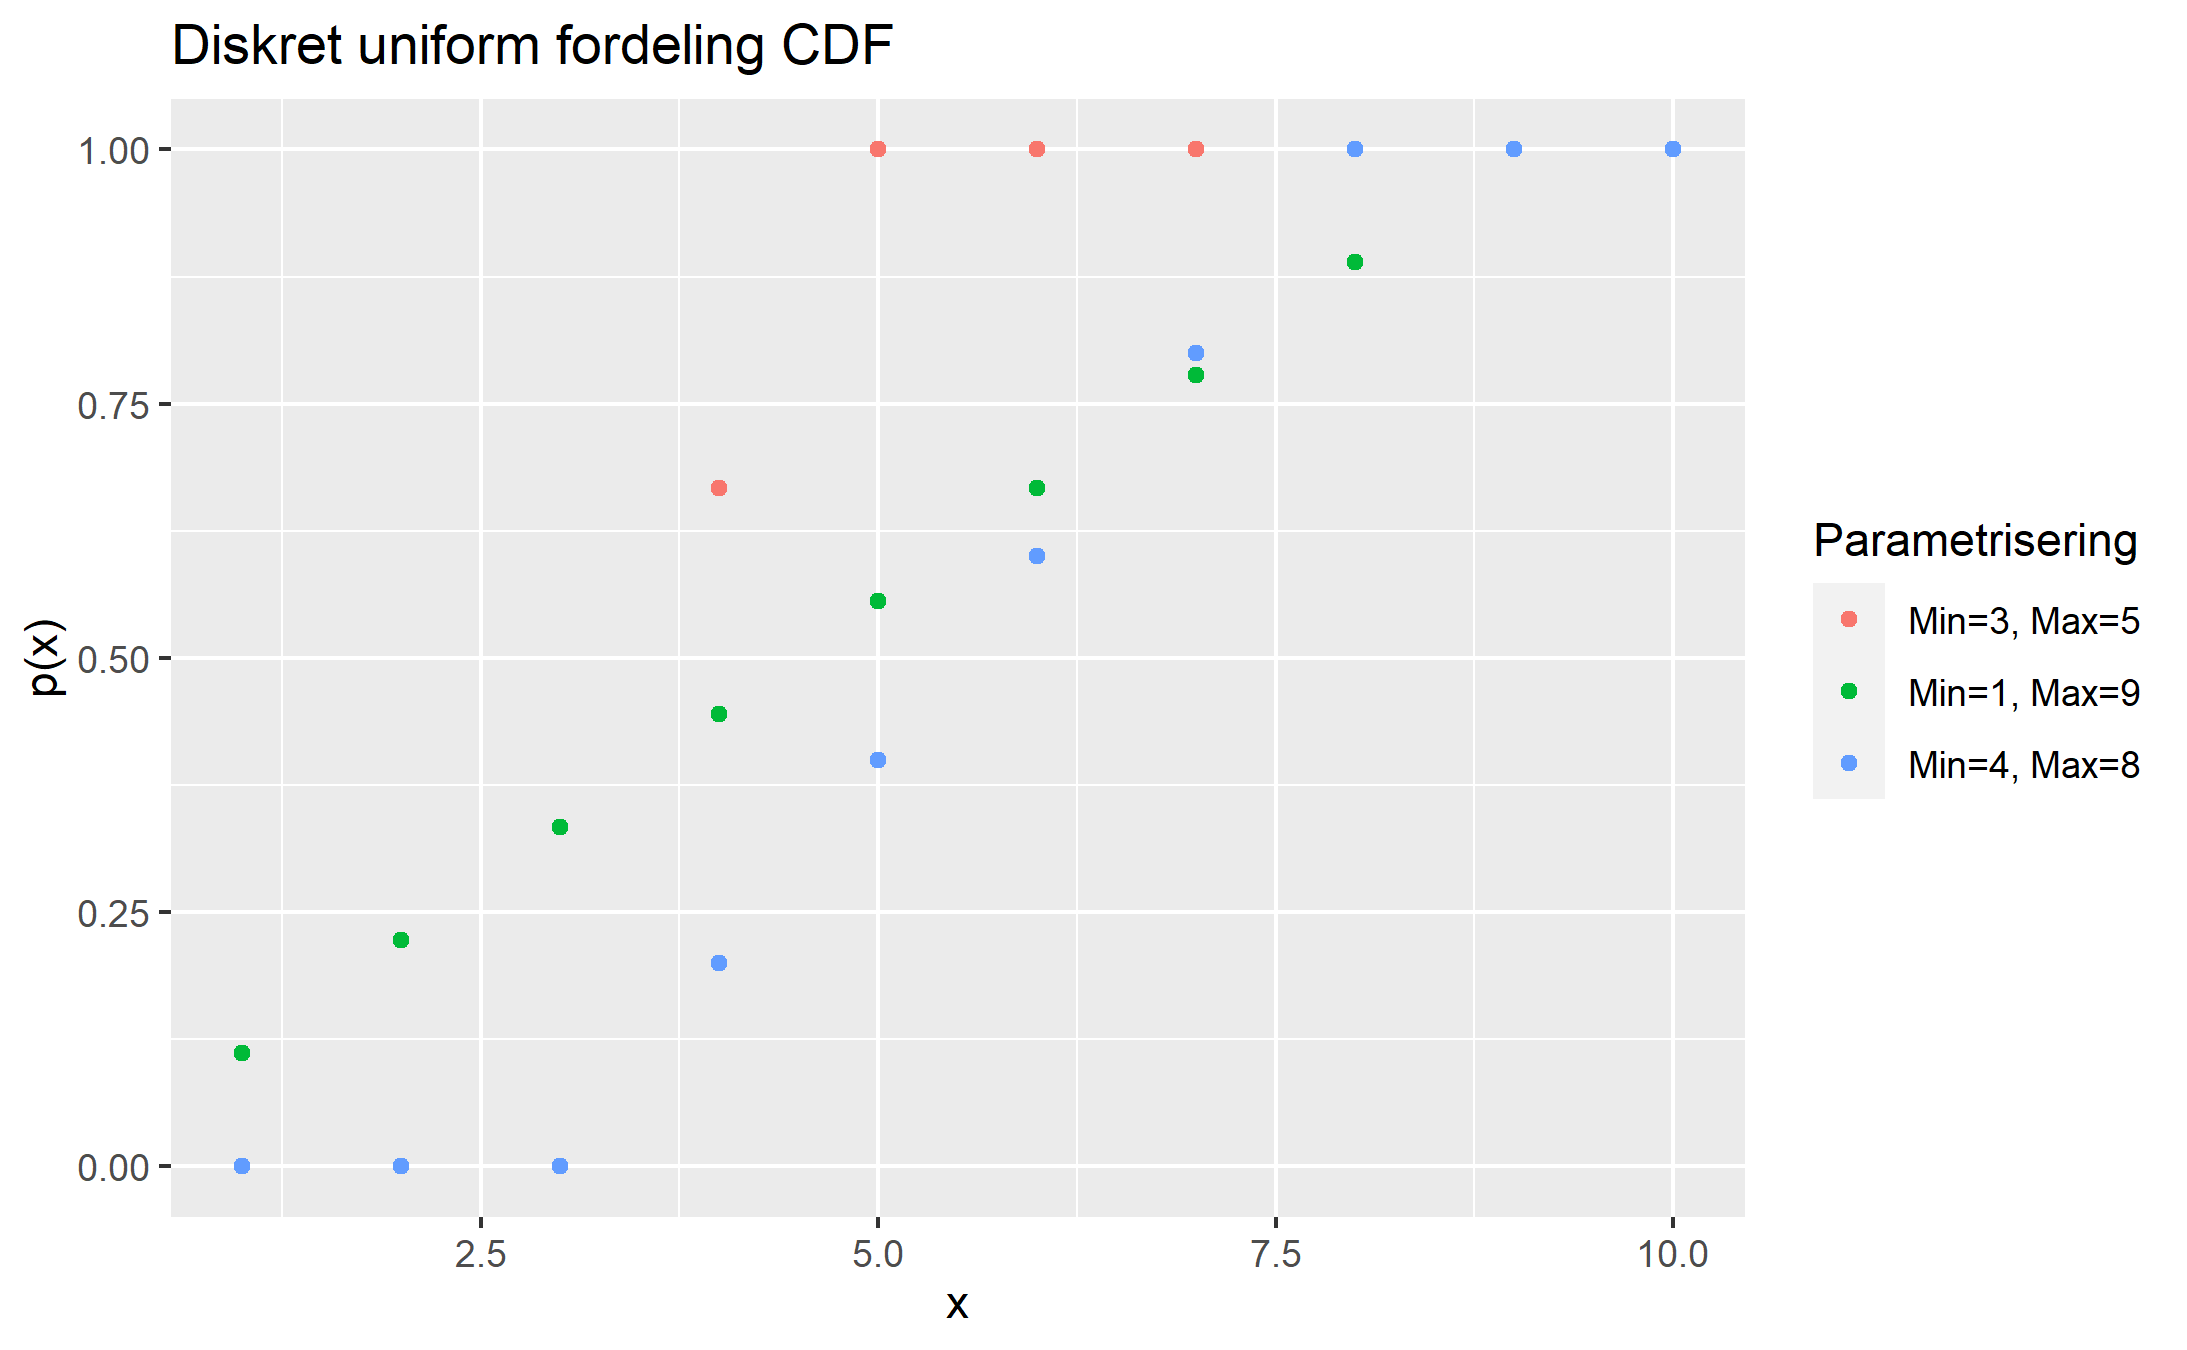
\includegraphics[width=\textwidth]{bilete/diskretuniformcdf.png}
  \end{minipage}
\end{figure}

Den diskrete uniforme fordelinga er ein fordeling der alle moglege utfall er like sannsynleg.

\begin{equation}
    f(x; a, b) = \frac{1}{n}, \qquad x \in \{a, a+1, \dots, b-1, b\}, \qquad n = b - a + 1, \qquad a \leq b
\end{equation}

\begin{equation}
    F(x; a, b) = P(X \leq x) = \frac{\lfloor x \rfloor - a + 1}{n}
\end{equation}

\begin{equation}
    E[X] = \frac{a + b}{2}, \qquad \text{Var}(X) = \frac{(b - a + 1)^2 - 1}{12}
\end{equation}

\section{Kontinuerlege sannsynlegheitsfordelingar}

\subsection{Definisjon}
Stokastiske variablar kan og vere kontinuerlige, dvs at utfallsrommet liggjer på tallinja og er uendeleg (ikkje tellbart uendeleg). Dette gjer det umogleg å lage ordna par $(x, f(x))$ på same måte som ein ikkje kan liste opp alle dei reelle tala ${\rm I\!R}$. 

Med kontinuerlege sannsynlegheitsfordelingar gir det då ikkje meining om å snakke om sannsynet for at $X = a$ då sannsynlegheita for at $X$ er nøyaktig lik $a$ er $0$, dette fordi det er uendeleg andre utfall. (Å intuitivt forstå dette blir overlatt til den enkelte som leser dette). Med kontinuerlige sannsynlegheitsfordelingar brukar me då intervall når me reknar ut sannsynet. 

Likevel kan sannsynlegheita for $X$ beskrivast med ein funksjon $f(x)$ som me kallar ein \textbf{sannsynlegheitstettleikfunksjon} (ikkje det samme som sannsynlegheitsmassefunksjon som det heiter i det diskrete tilfellet). Denne funksjonen må følge desse krava for å vere ein gyldig sannsynlegheitstettleikfunksjon:

\begin{enumerate}
    \item $f(x) \geq 0$, for alle $x \in {\rm I\!R}$.
    \item  $\int_{-\infty}^{\infty} f(x) \, dx = 1$
    \item $P(a < X < b) = \int_{a}^{b} f(x) \, dx$
\end{enumerate}

Krava over betyr at vi definerer arealet under funksjonen til å vere sannsynlegheita. Derfor må arealet under heile funksjonen vere $1$. Sannsynlegheita for at $X$ er mellom $a$ og $b$ er då arealet under grafen frå $a$ til $b$ og derfor må me integrere funksjonen.

På same måte som den kumulative funksjonen i det diskrete tilfellet, har me ein kumulativ funksjon for kontinuerlege stokastiske variablar. Den er definert slik:

\begin{equation}
    F(x) = P(X \leq x) = \int_{-\infty}^{t} f(t) \, dt, \qquad -\infty < x < \infty
\end{equation}

Denne funksjonen gir då arealet under heile funksjonen fram til x. Som då er sannsynlegheita for at $X$ er mindre eller lik $x$.

\textbf{Forventingsverdi} $E[X]$ og \textbf{Varians} $\text{Var}(X)$ er også definert for kontinuerlige stokastiske variablar. Desse reknar me ut slik

\begin{equation}
    \mu = E[X] = \int_{\infty}^{\infty} xf(x) \, dx
\end{equation}

\begin{equation}
    \sigma^2 = \text{Var}(X) = E[(X-\mu^2)] = E[X^2] - E[X]^2 = \int_{\infty}^{\infty} (x-\mu)f(x) \, dx = \int_{\infty}^{\infty} x^2 f(x) \, dx - \mu^2 
\end{equation}

\subsection{Uniform fordeling}
\begin{figure}[H]
  \centering
  \begin{minipage}[b]{0.49\textwidth}
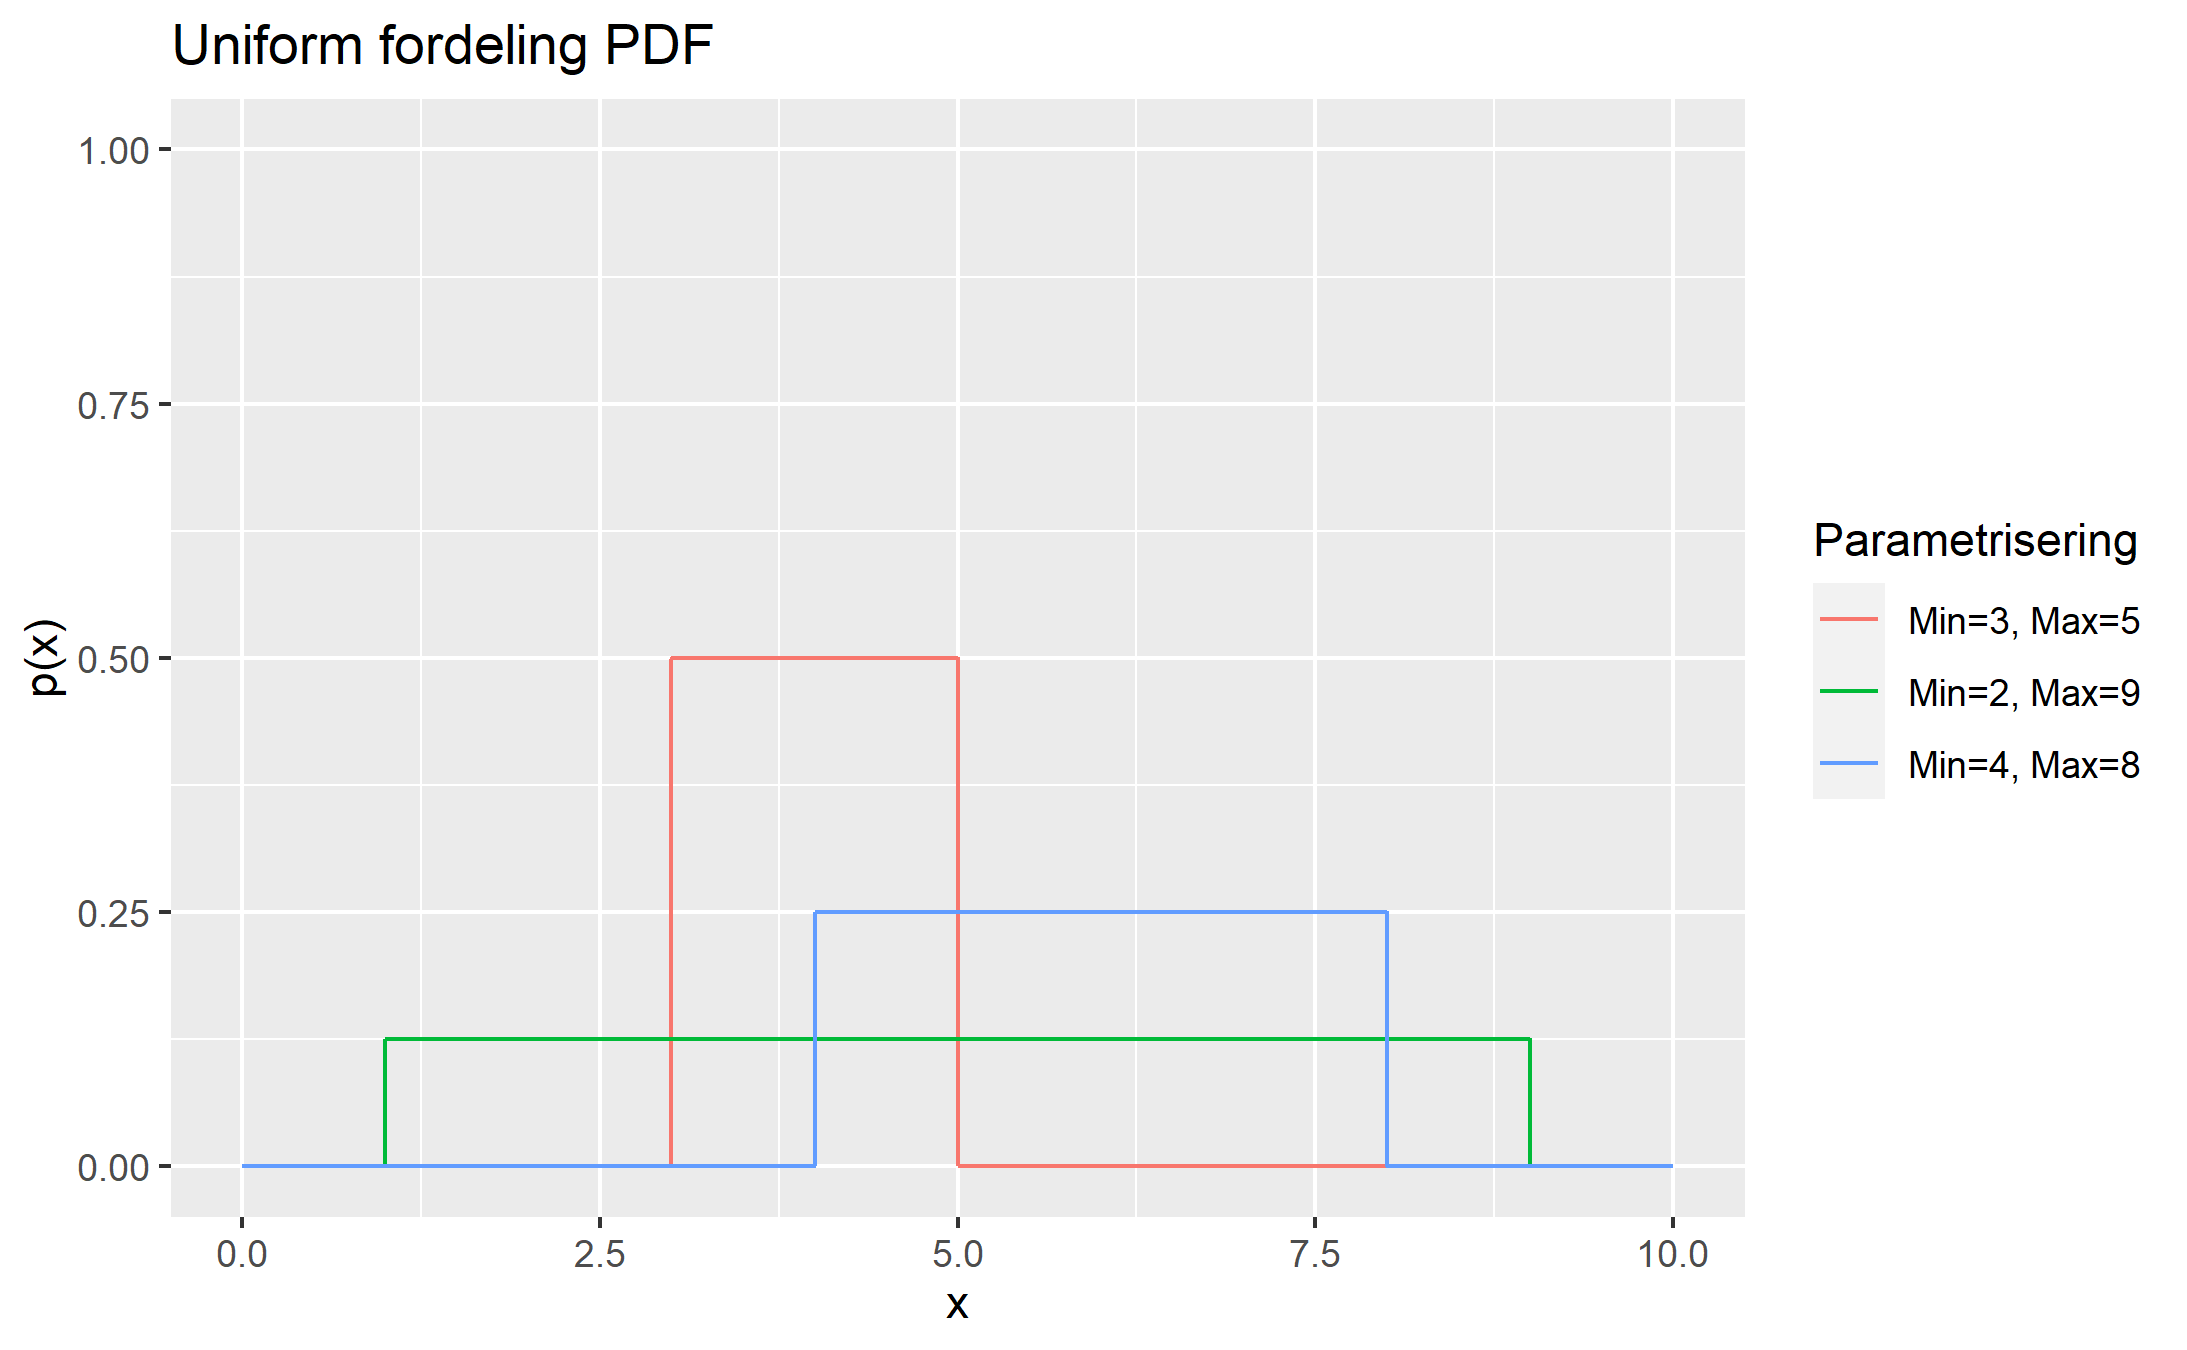
\includegraphics[width=\textwidth]{bilete/unifpdf.png}
  \end{minipage}
  \hfill
  \begin{minipage}[b]{0.49\textwidth}
    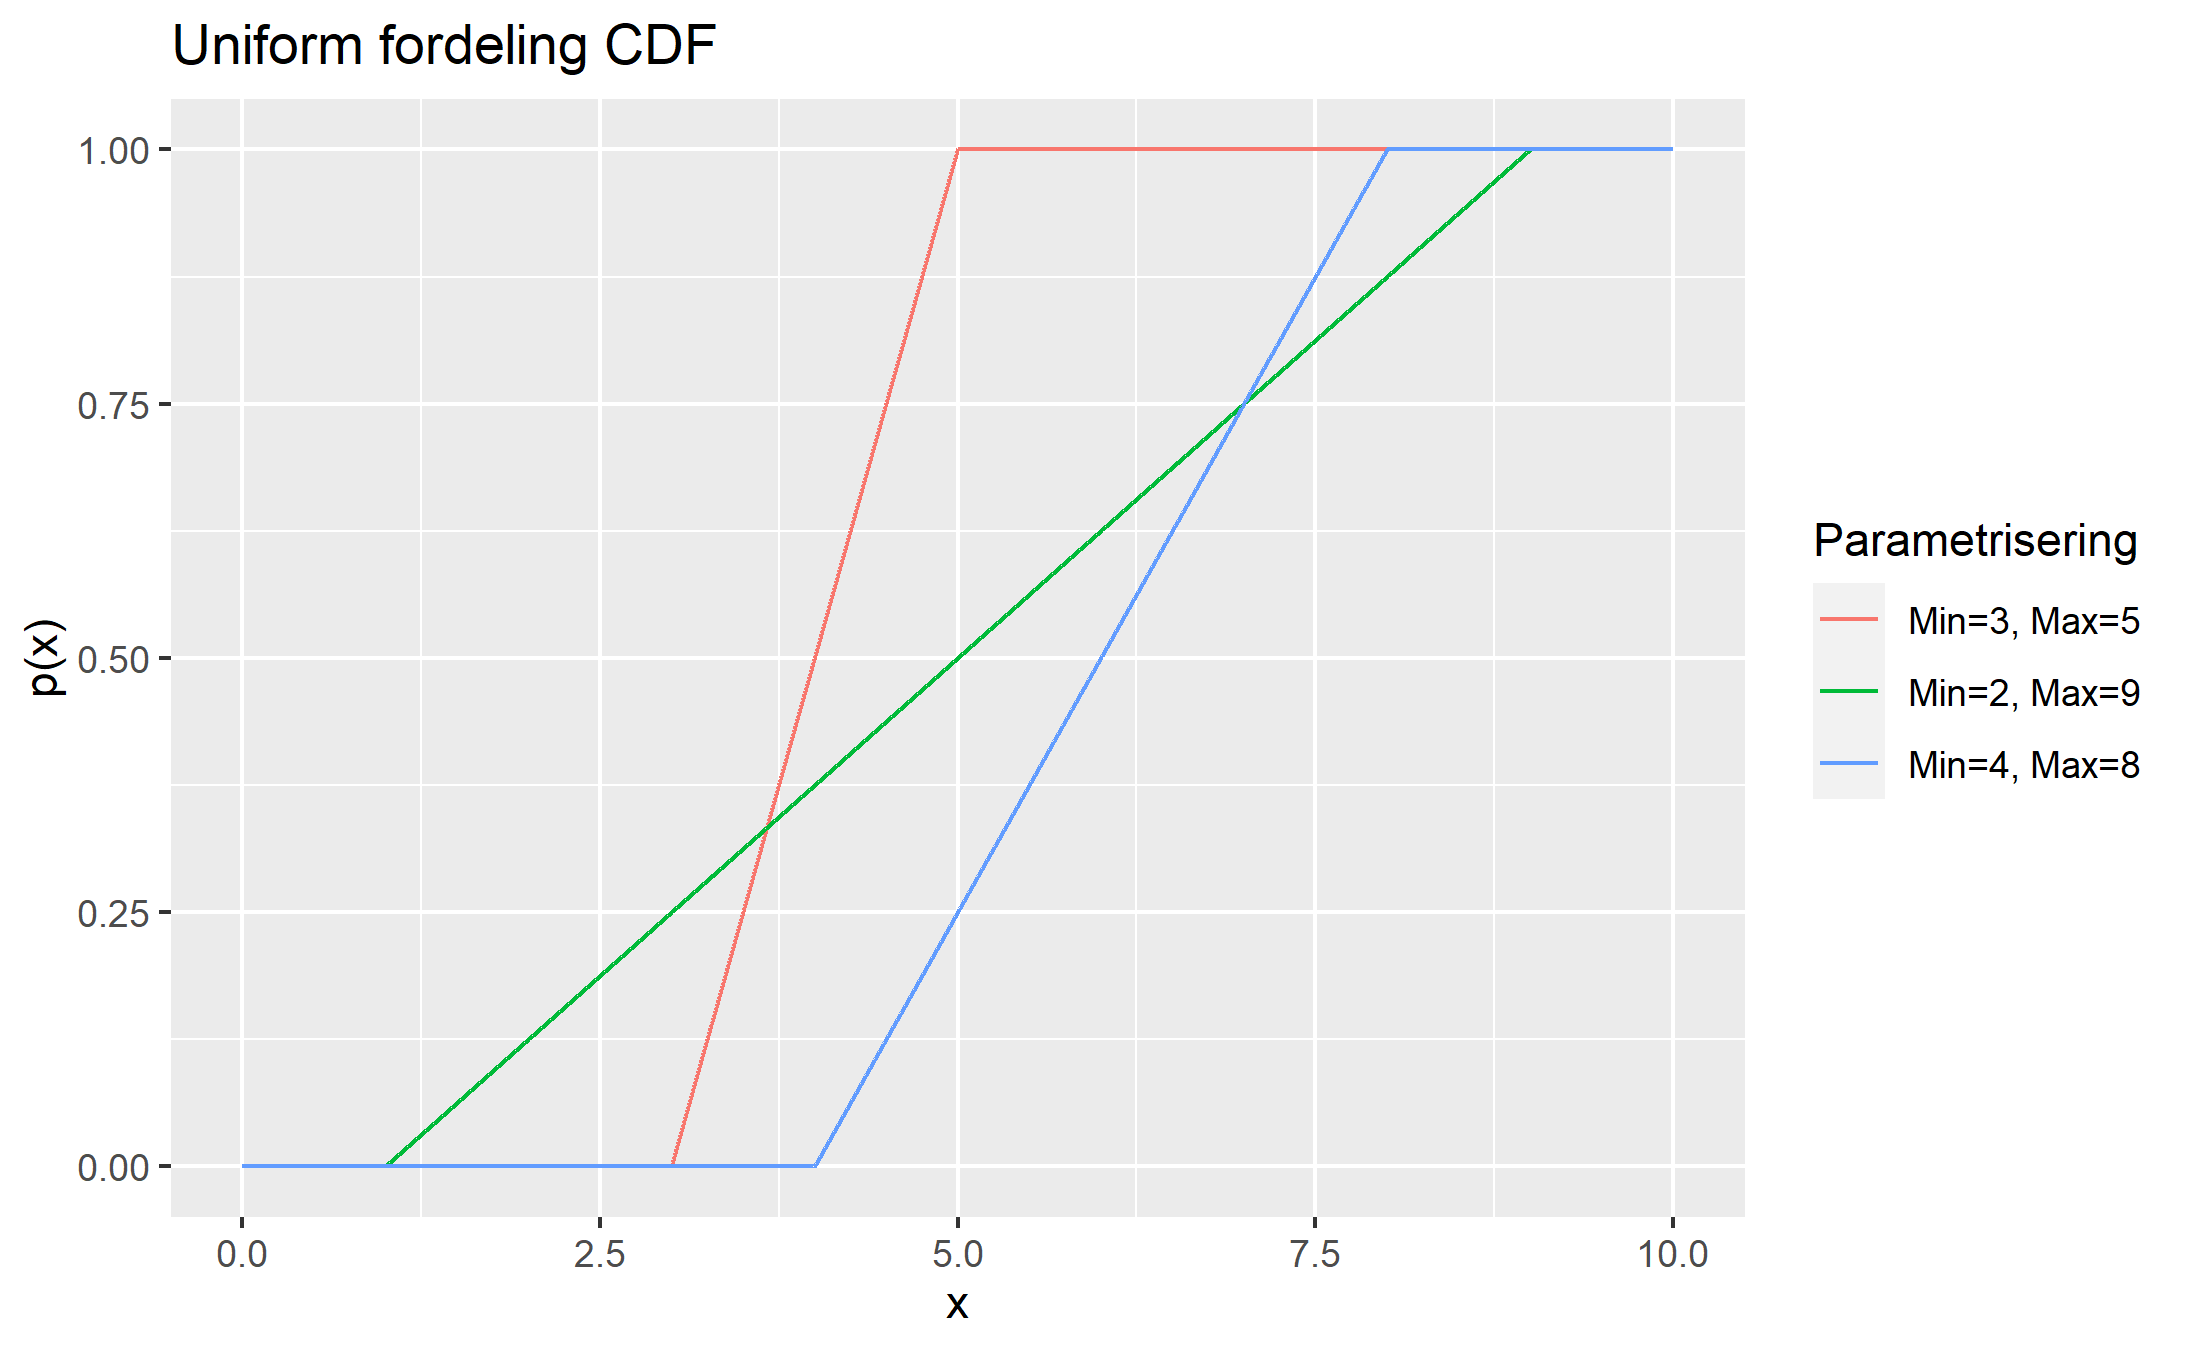
\includegraphics[width=\textwidth]{bilete/unifcdf.png}
  \end{minipage}
\end{figure}

\begin{equation}
    f(x; a, b) = u(x; a, b) = 
    \begin{cases}
    \frac{1}{b - a}, & x \in [a, b] \\
    0, & \text{Ellers}
    \end{cases}
\end{equation}

\begin{equation}
    F(x; a, b) = P(X \leq x) = 
    \begin{cases}
        0, & x < a \\
        \frac{x-a}{b-a}, & x \in [a, b] \\
        1, & x > b
    \end{cases}
\end{equation}

\begin{equation}
    E[X] = \frac{a + b}{2}, \qquad \text{Var}(X) = \frac{(b-a)^2}{12}
\end{equation}

\subsection{Normalfordeling}
\begin{figure}[H]
  \centering
  \begin{minipage}[b]{0.49\textwidth}
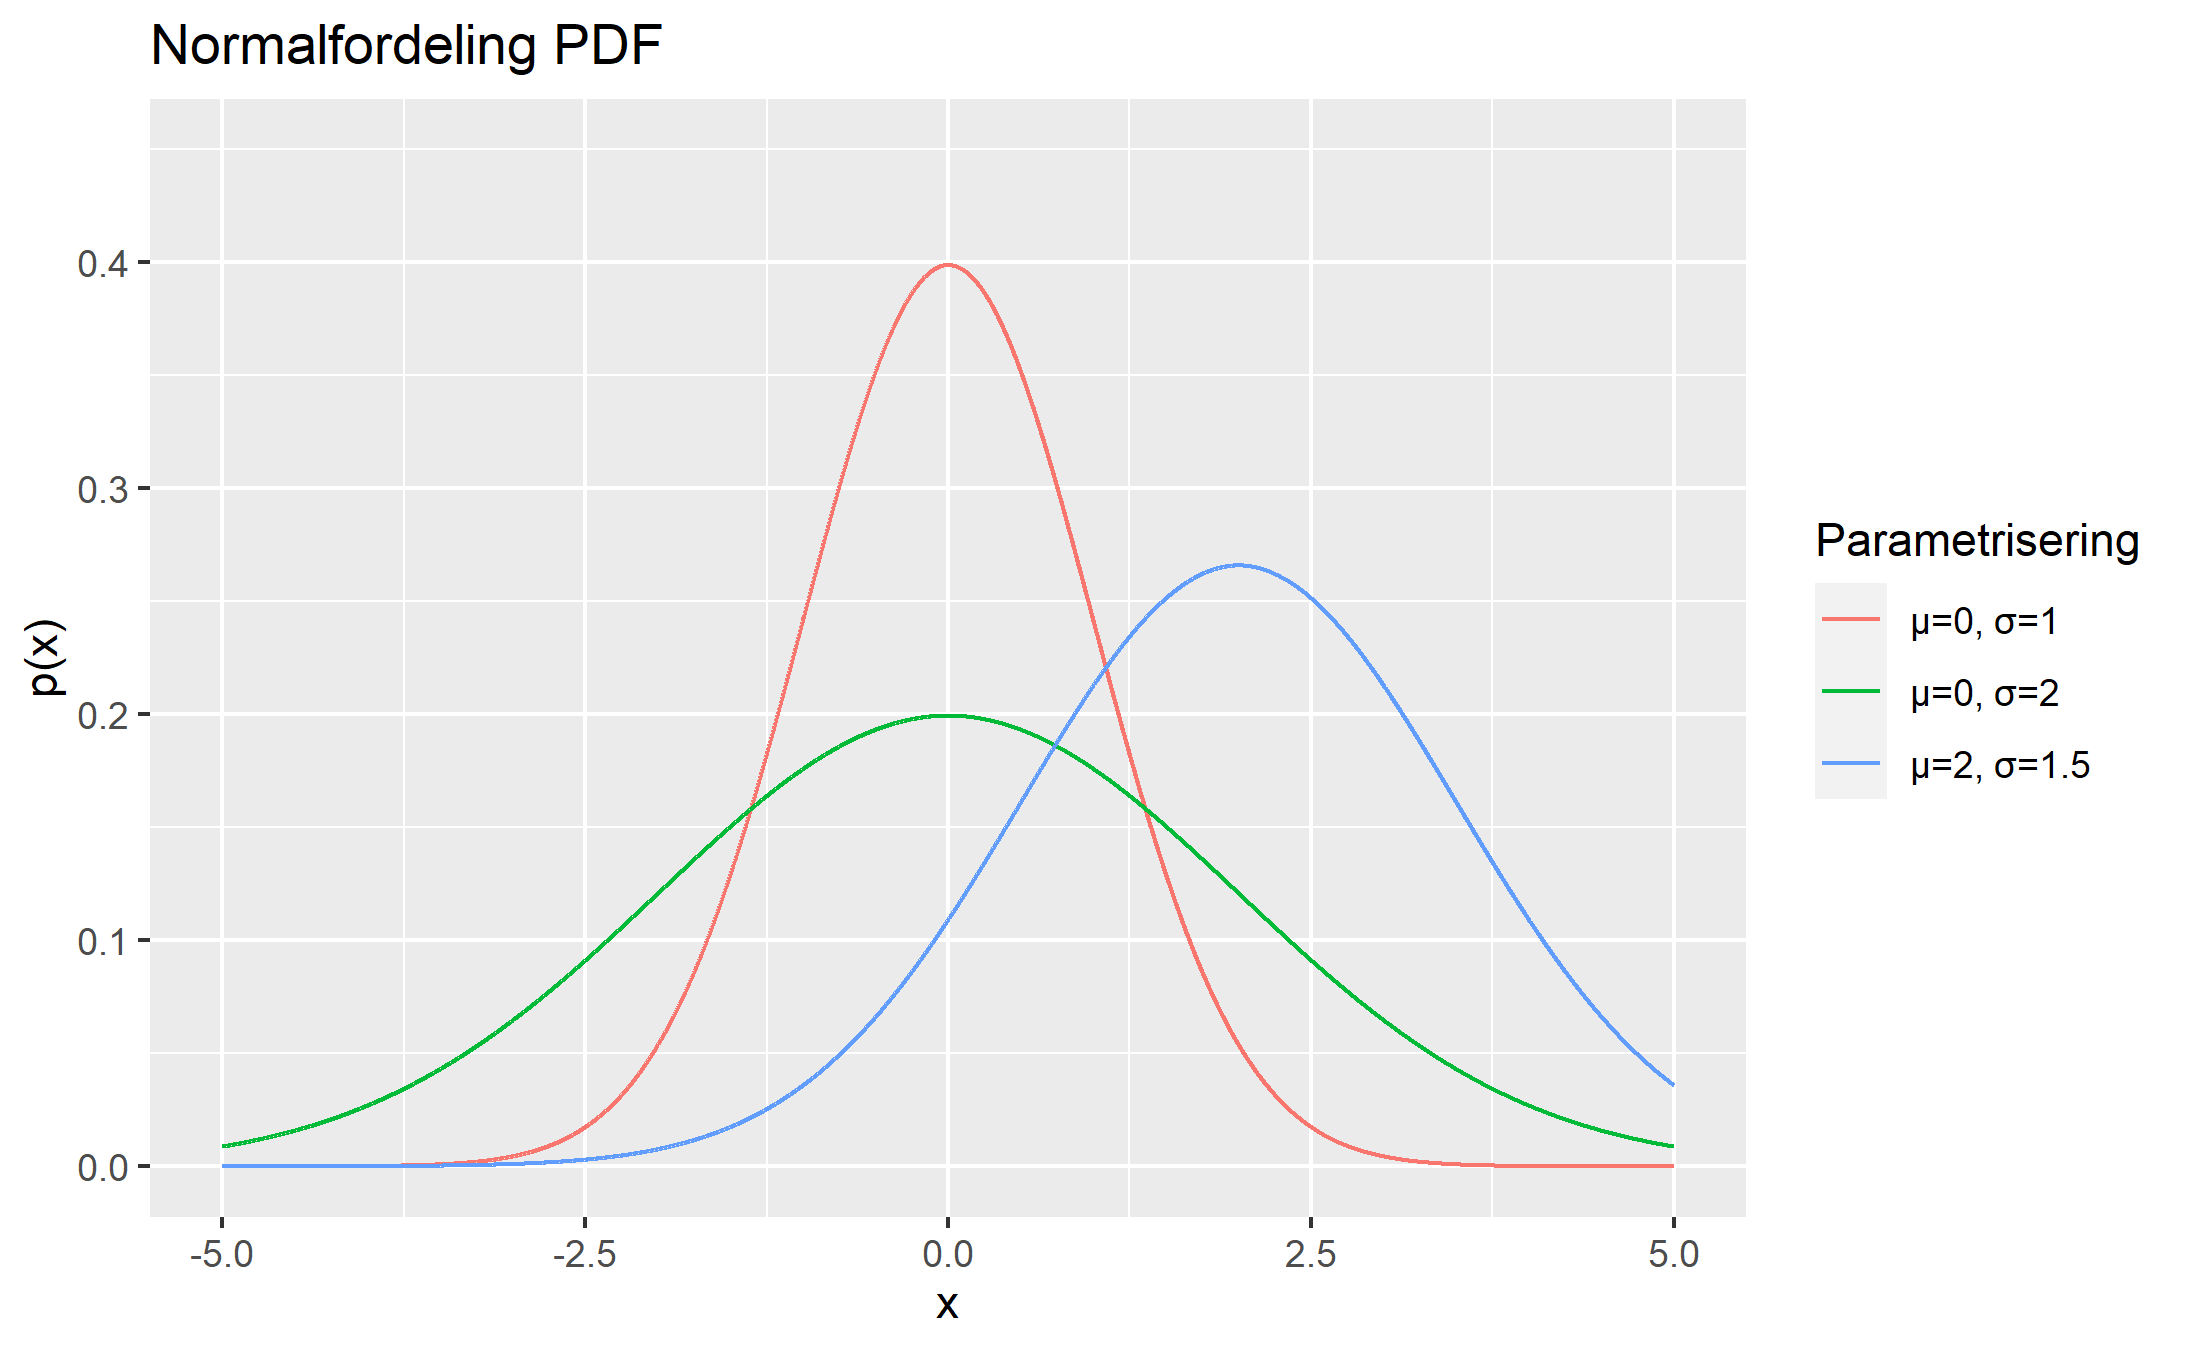
\includegraphics[width=\textwidth]{bilete/normpdf.png}
  \end{minipage}
  \hfill
  \begin{minipage}[b]{0.49\textwidth}
    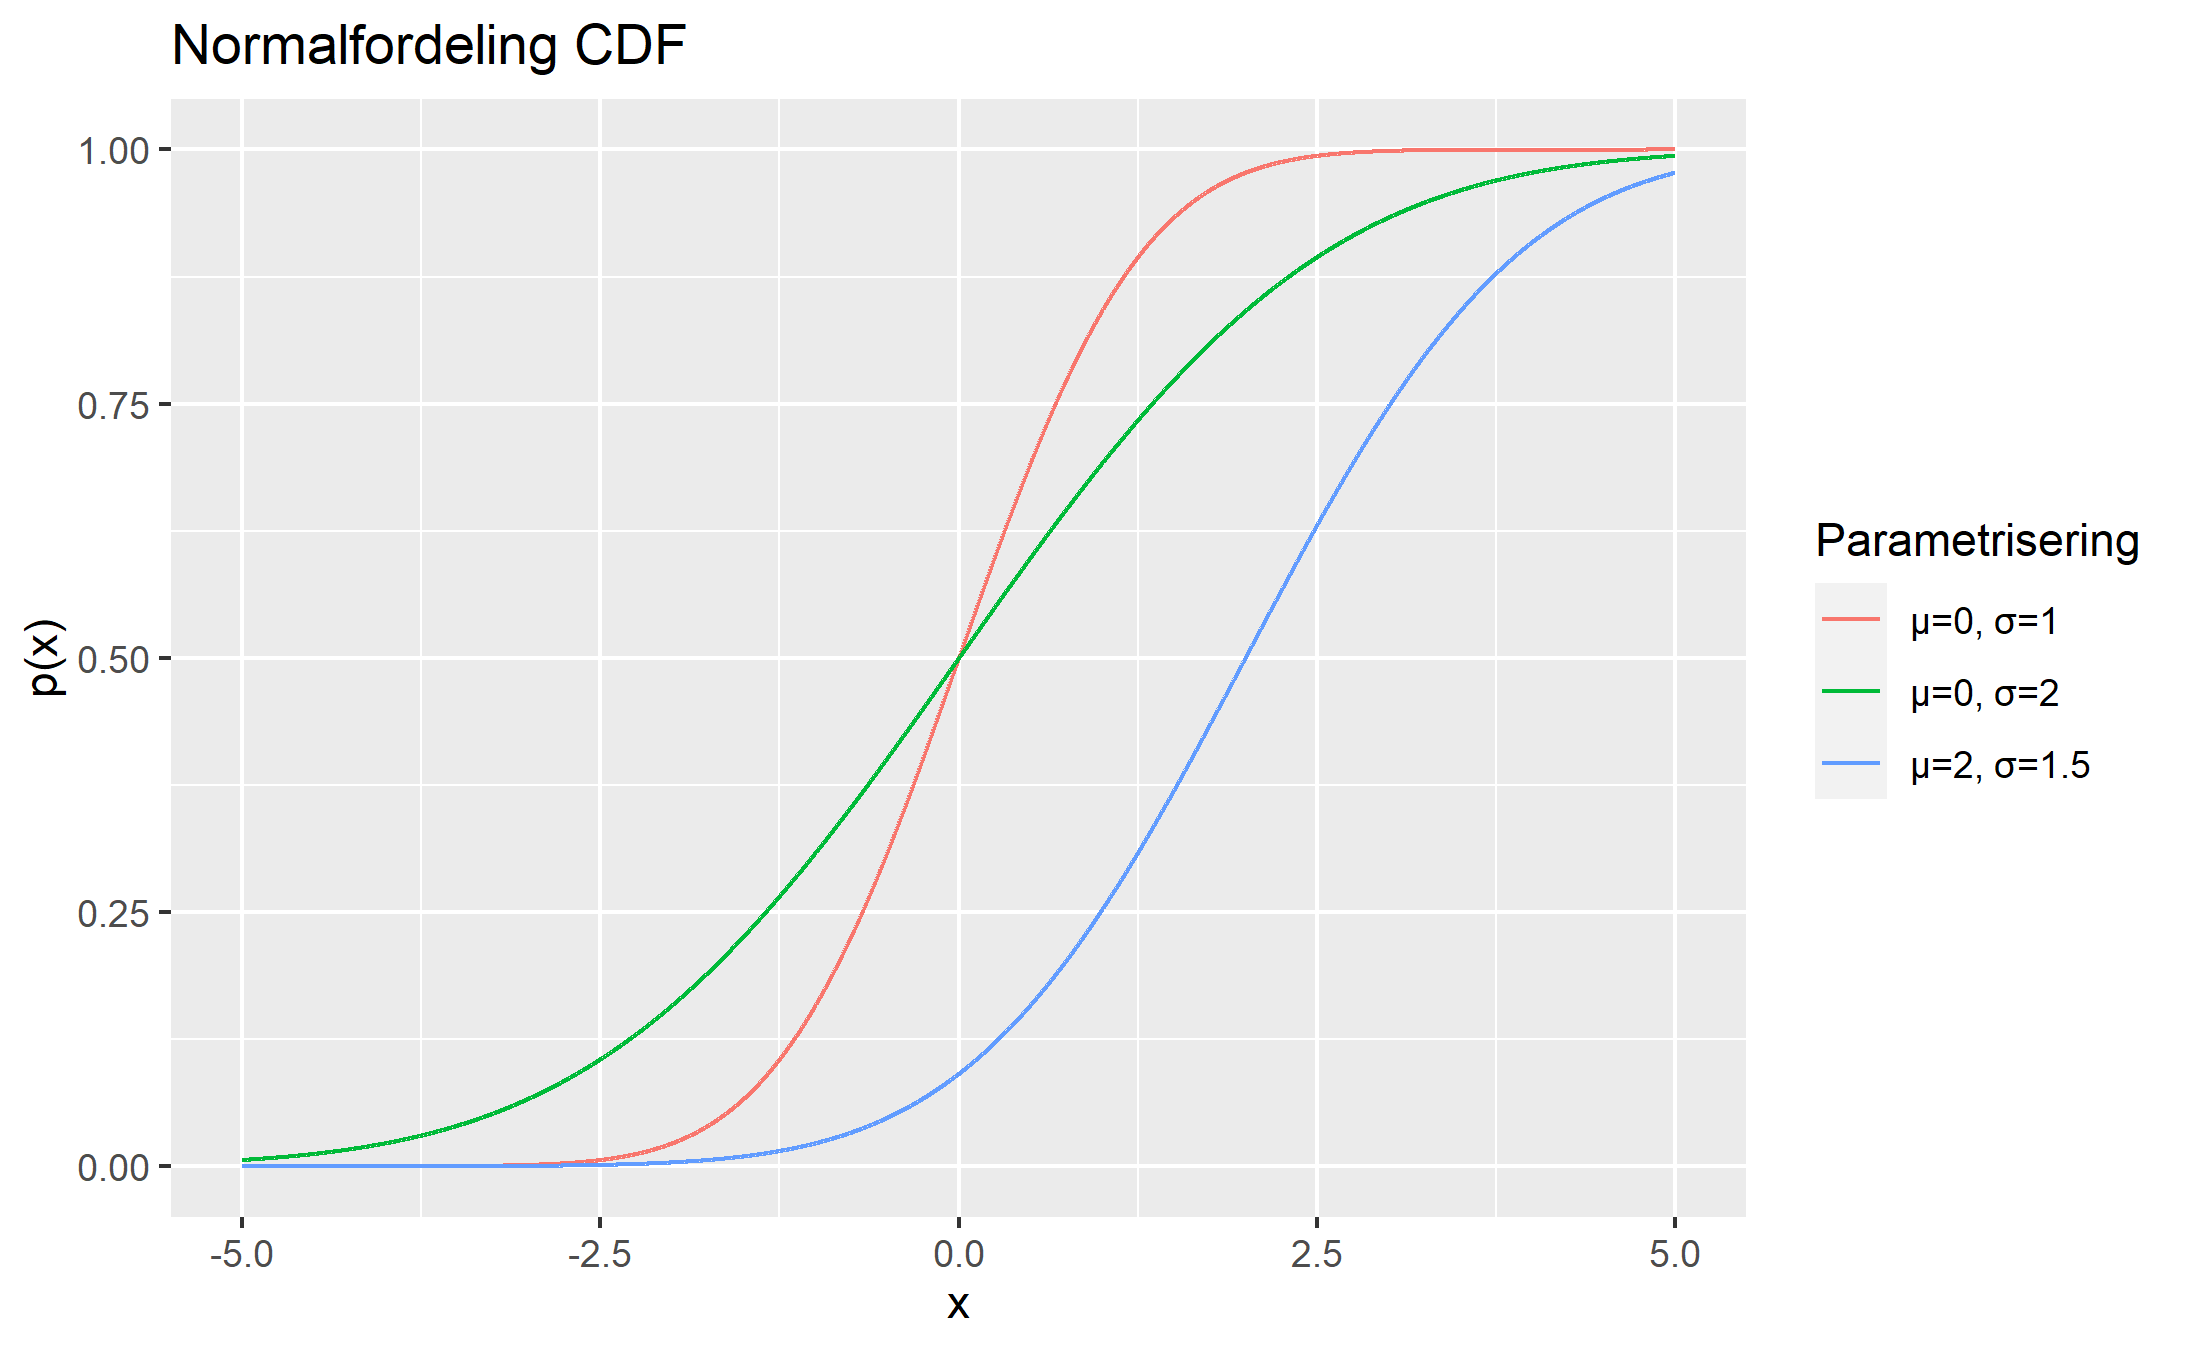
\includegraphics[width=\textwidth]{bilete/normcdf.png}
  \end{minipage}
\end{figure}

\begin{equation}
    f(x; \mu, \sigma) = n(x; \mu, \sigma) = \frac{1}{\sqrt{2\pi}\sigma} e^{-\frac{1}{2\sigma^2}(x-\mu)^2}
\end{equation}

\begin{equation}
    F(x; \mu, \sigma) = P(X \leq x) = \boldsymbol{\phi}\left(\frac{x - \mu}{\sigma}\right)
\end{equation}

\begin{equation}
    E[X] = \mu, \qquad \text{Var}(X) = \sigma^2
\end{equation}

\subsubsection{Normalfordelingen i praksis}\label{chap:normpraksis}

Når ein har ein massetettleiksfunksjon $f(x)$ for ein fordeling og ein ynskjer å finne den kumulative tettleiksfunsjonen $F(x)$ kan ein normalt benytte seg av $F(x) = \int_{-\infty}^{x} f(t) \,dt$. Men med
$f(x; \mu, \sigma)$ er dette vanskeleg for avgrensa område under grafen. Ein kan heldigvis jobbe seg rundt dette med å lage ein tabell for standard normalfordeling.  Alle normalfordelingar kan skalerast til ein standard normalfordeling og derfor kan ein nytte ein tabell for standard normalfordeling for å gjere utrekningar på alle normalfordelingar. Omgjering av ein normalfordeling gjer ein slik:

\begin{equation}
    Z = \frac{X - \mu}{\sigma}
\end{equation}

Der $X$ er ein vilkårleg normalfordeling. 

\subsection{Gammafordelingen}
\begin{figure}[H]
  \centering
  \begin{minipage}[b]{0.49\textwidth}
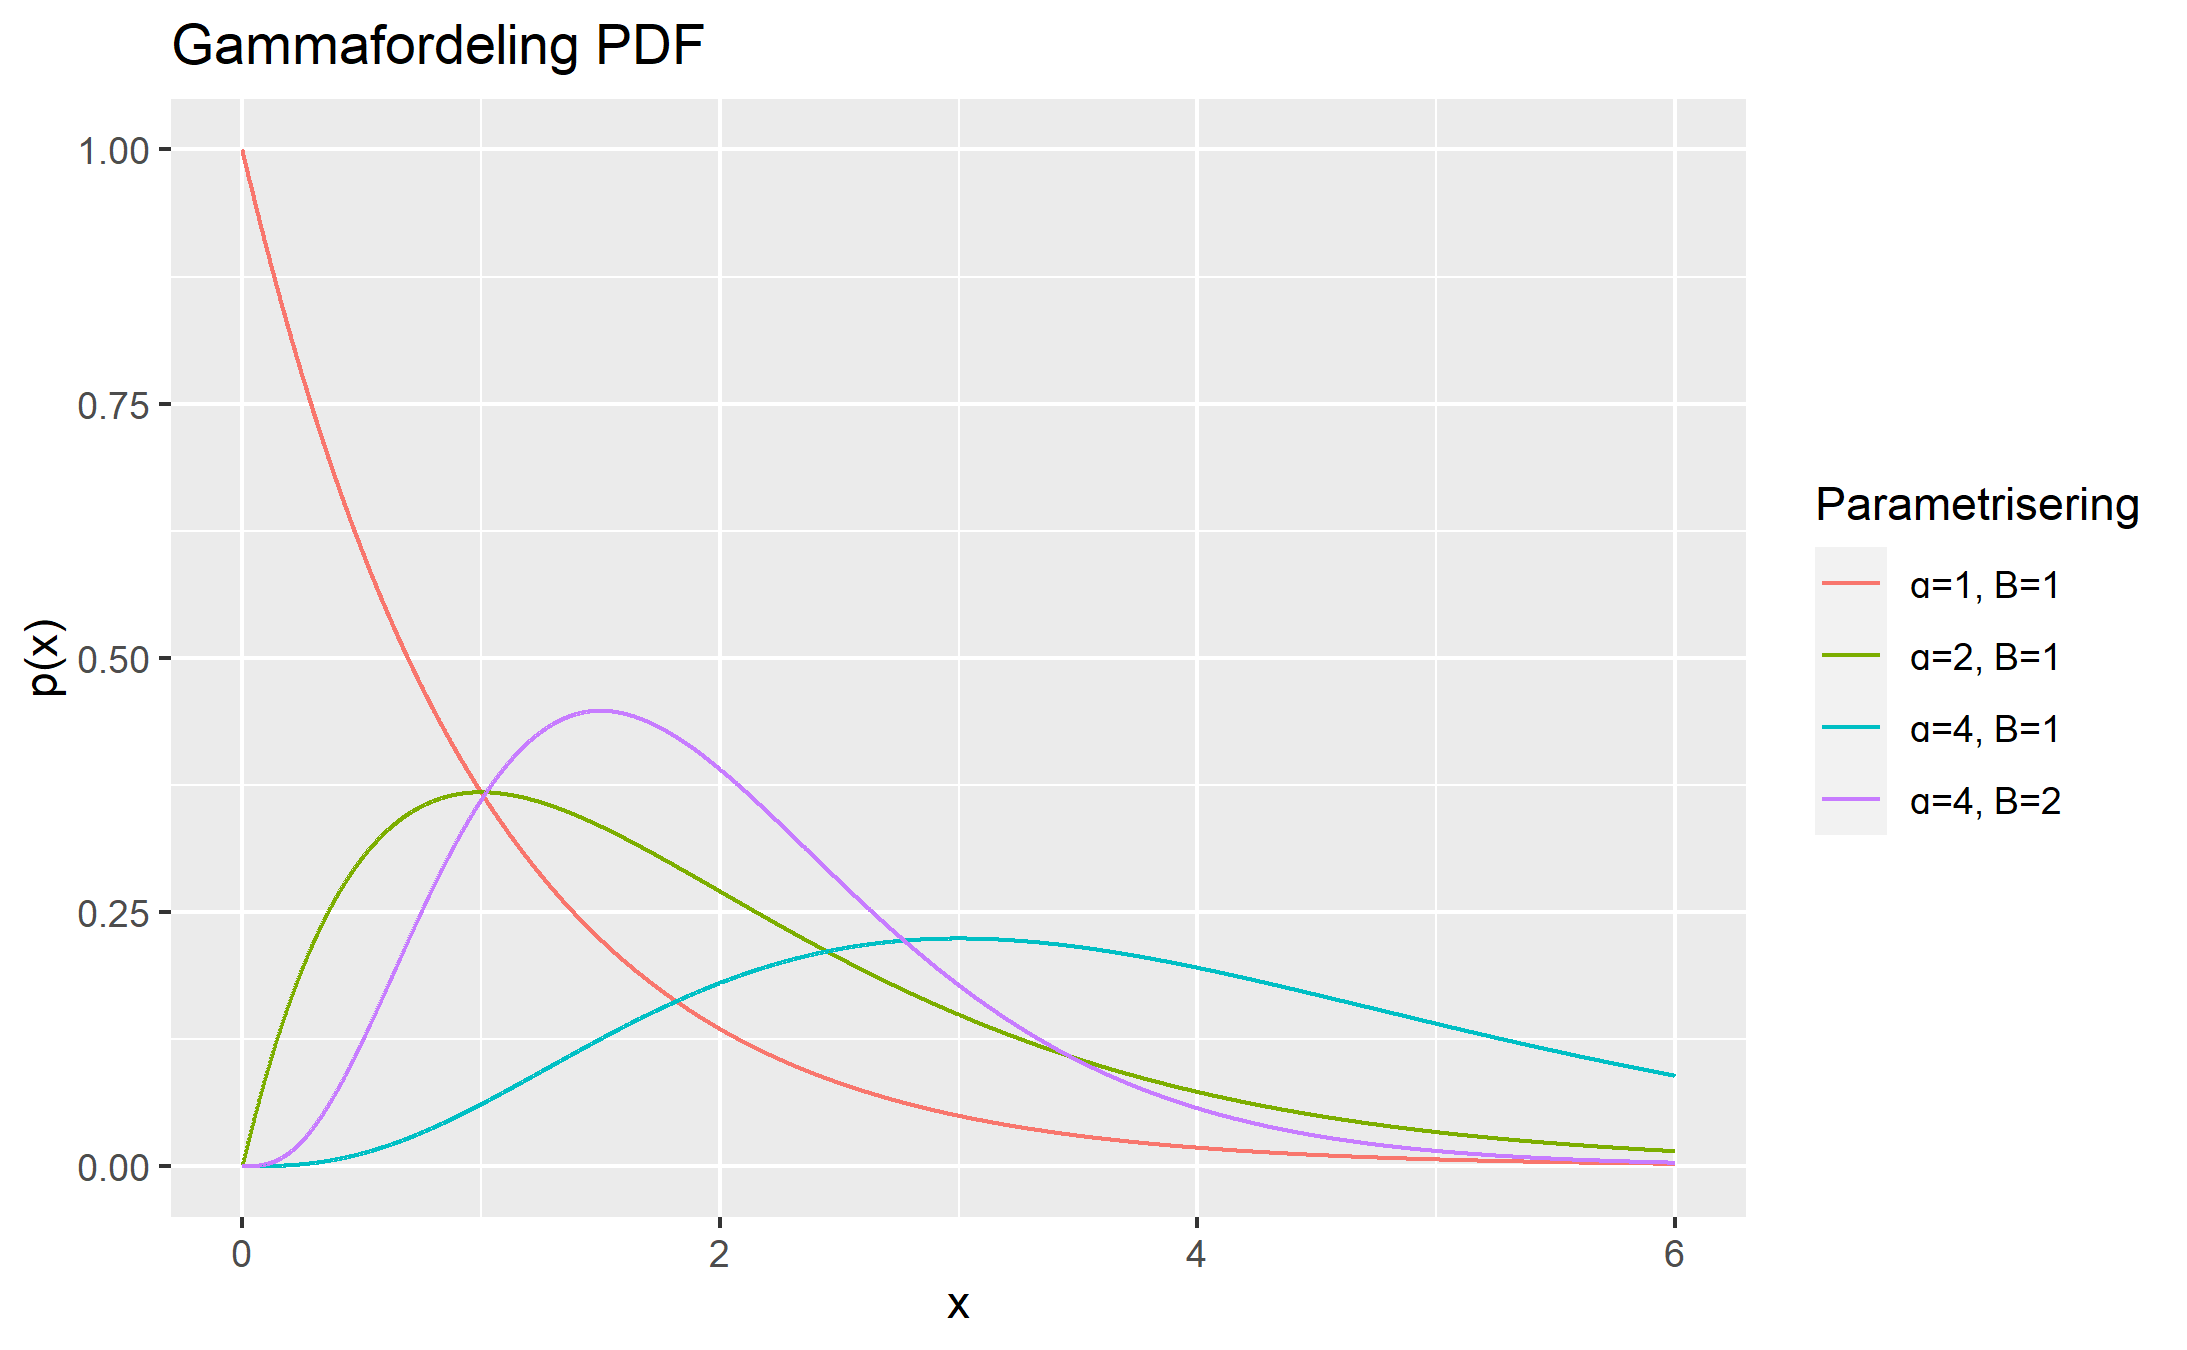
\includegraphics[width=\textwidth]{bilete/gammapdf.png}
  \end{minipage}
  \hfill
  \begin{minipage}[b]{0.49\textwidth}
    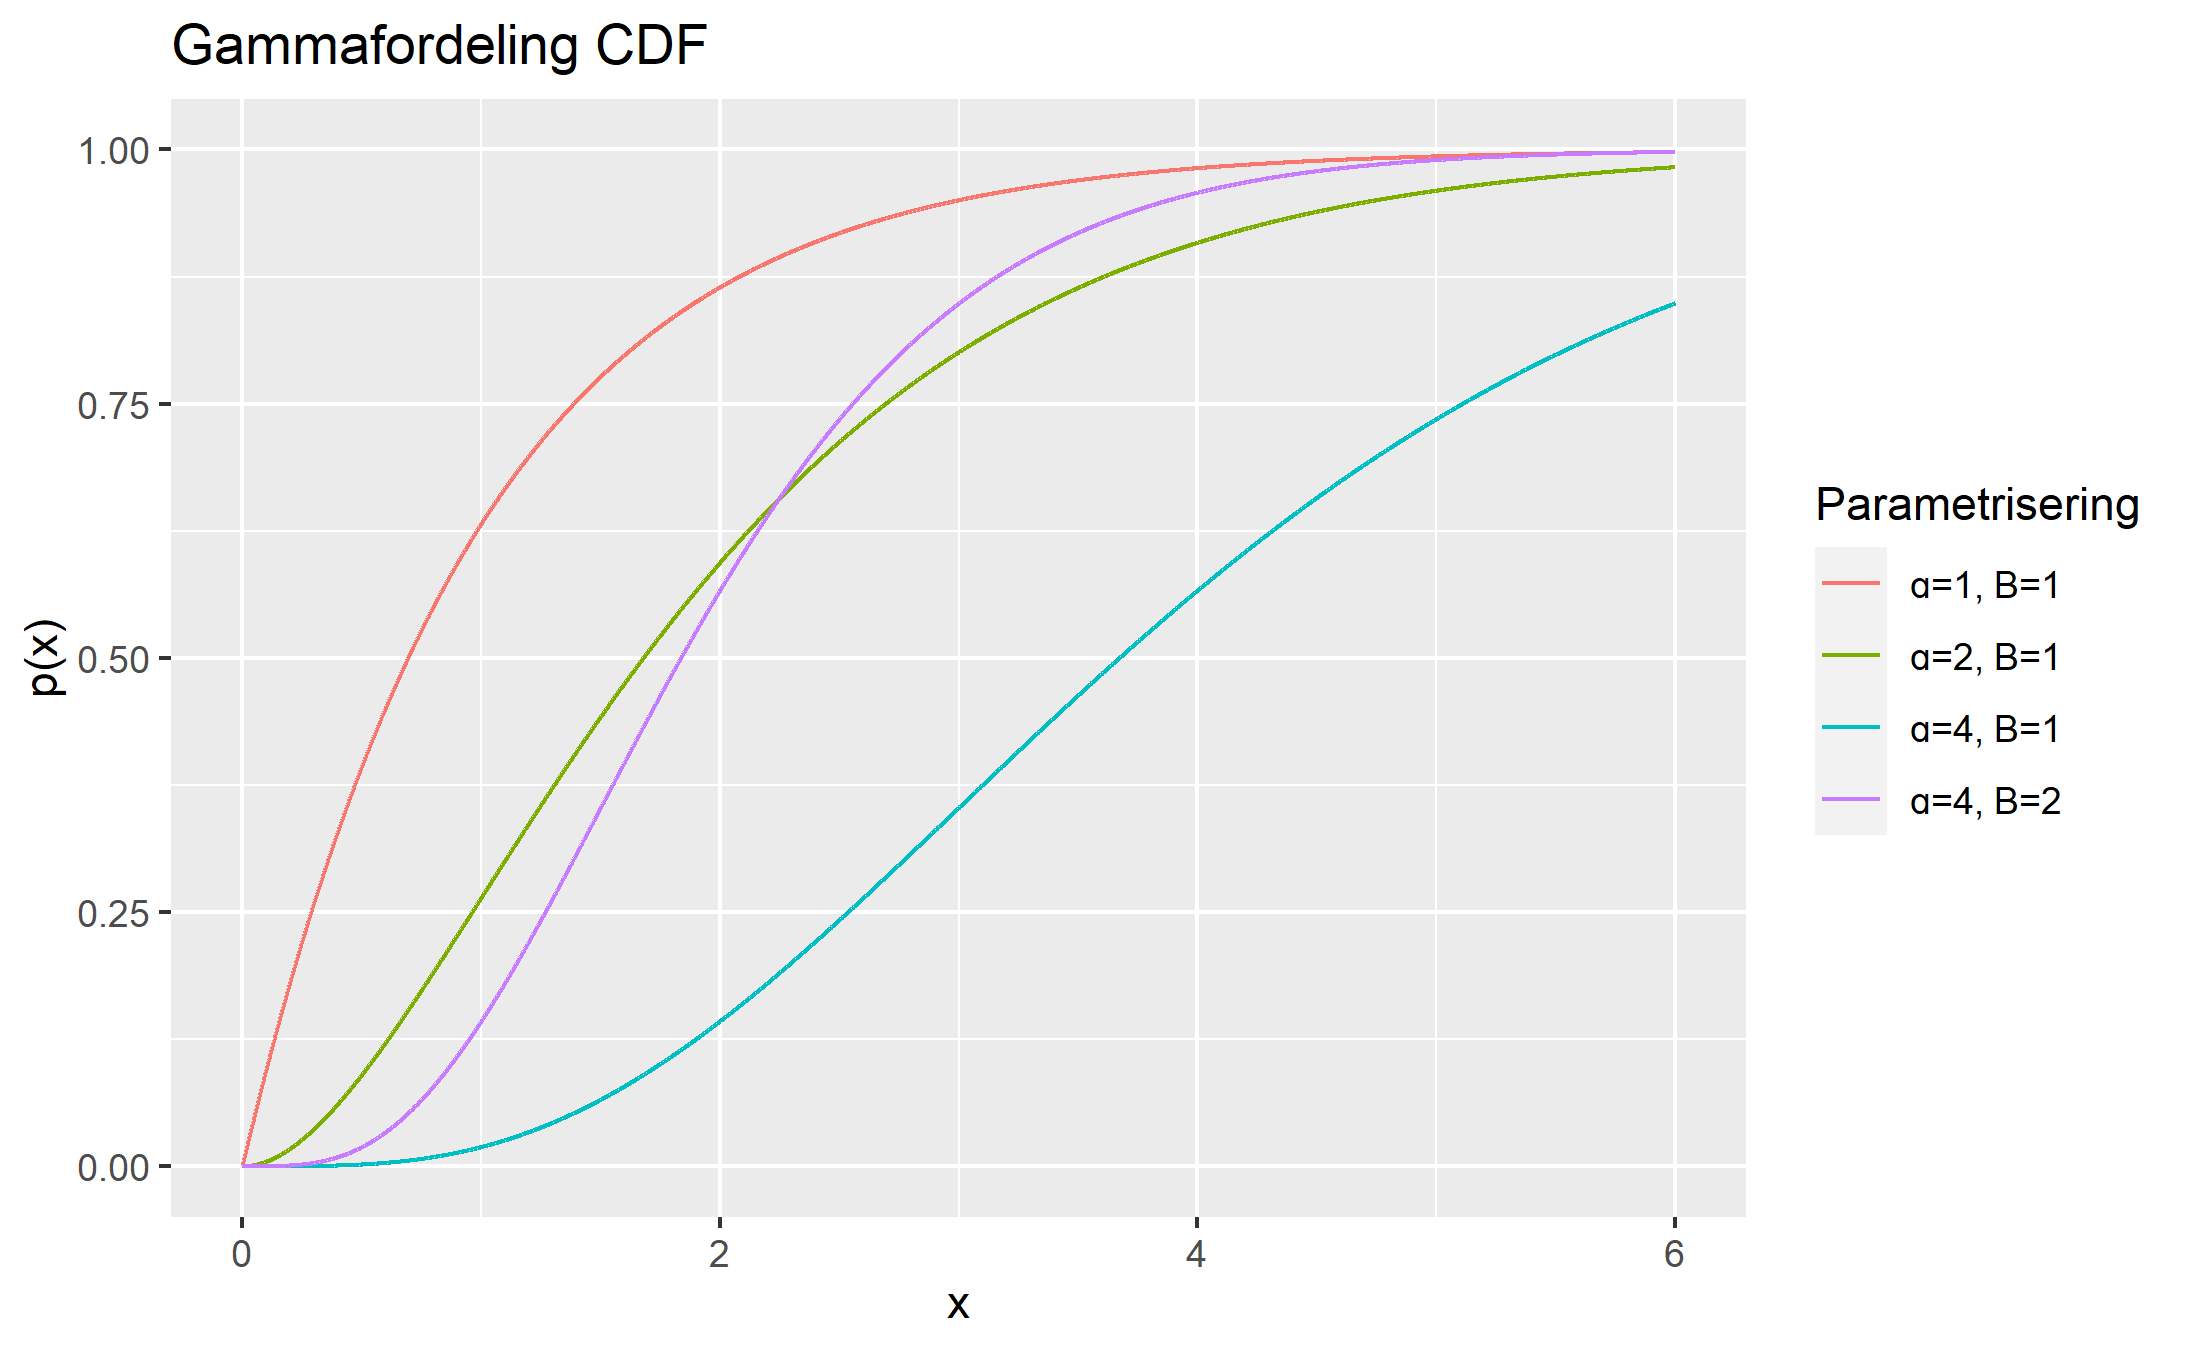
\includegraphics[width=\textwidth]{bilete/gammacdf.png}
  \end{minipage}
\end{figure}

\textbf{Obs: } Gammafordelingen har 3 parametriseringar som er vanlege

\begin{enumerate}
    \item Med formparameter $k$ og skalaparameter $\theta$ \label{pointgamma}
    \item Med formparameter $\alpha = k$ og hastigheitsparameter $\beta = \frac{1}{\theta}$ \label{pointgamma2}
    \item Med formparameter k og gjennomsnittsparameter $\mu = k\theta = \frac{\alpha}{\beta}$
\end{enumerate}

Der me nyttar parametriseringa i punkt \ref{pointgamma}. Det er derfor viktig å merke seg at når ein jobbar med gammafordelingen (og fordelingar generelt) at det er forskjellige parametriseringar og at ein må vere sikker på at ein har tatt i bruk korrekt parametrisering.

For å skape ekstra forvirring nyttar forfattaren og emnelæraren seg av $(k, \theta)$ parametrisering men bruker bokstavane $\alpha$ og $\beta$ for desse parametra. Dette må ikkje bli forveksla med $(\alpha, \beta)$ parametriseringa i punkt \ref{pointgamma2}. I dete faget er det derfor desse formlane som gjelder

\begin{equation}
    f(x; \alpha, \beta) = 
    \begin{cases}
        \frac{1}{\beta^\alpha \Gamma(\alpha)}x^{\alpha - 1}e^{-x/\beta} & x \in [0, \infty] \\
        0 & \text{Ellers}
    \end{cases}
\end{equation}

\begin{equation}
    F(x; \alpha, \beta) = \frac{1}{\Gamma(\alpha)}\gamma\left(\alpha, \frac{x}{\beta}\right)
\end{equation}

Der $\gamma$ er den inkomplette-gammafunksjonen \cite{wiki:incomgamma} og $\Gamma$ er gammafunksjonen \cite{walpole2012probability}. Desse reknar me i praksis ut vha verktøy som R. 

\begin{equation}
    E[X] = \alpha\beta, \qquad \text{Var}(X) = \alpha\beta^2
\end{equation}

\subsubsection{Spesialtilfelle}

Gammafordelingen er ein fleksibel fordeling som har mange bruksområde. Det finnast 2 spesialtilfelle av gammafordelingen som er veldig etablert og som me ser på som sine eigne fullverdige fordelingar

\begin{enumerate}
    \item $\alpha = 1$ gir oss eksponensialfordelinga\ref{eksp} med $\beta$ som skalaparemeter\ref{eksp:skala}.
    \item $\alpha = \nu/2$ og $\beta = 2$ gir oss $\chi^2$-fordelinga
\end{enumerate}

\subsubsection{Relasjon til poissonprosessen}
Sjå kapittel \ref{memless} for å lese om eksponensialfordelingen og dens minnelausheit.

Poissonfordelingen, eksponensialfordelingen og gammafordelingen er 3 viktige fordelingar som alle beskriver visse eigenskapar i poissonprosessen. Hugs at eksponensialfordelinga er ein gammafordeling med formparameter $\alpha = 1$. Tiden det tar mellom to poissonhendingar/tiden frå start til den første hendinga er eksponensialfordelt. Gammafordelingen generaliserer dette og formparameteren $\alpha$ kan bli tenkt på som antalet hendingar me ventar på.

Tiden det då tar for at $n$ poissonhendingar skal ta plass er då gammafordelt med formparameter $\alpha = n$. Ein lineærkombinasjon av fleire eksonensialfordelingar er derfor gammafordelt.

\subsection{Eksponensialfordeling}\label{eksp}
\begin{figure}[H]
  \centering
  \begin{minipage}[b]{0.49\textwidth}
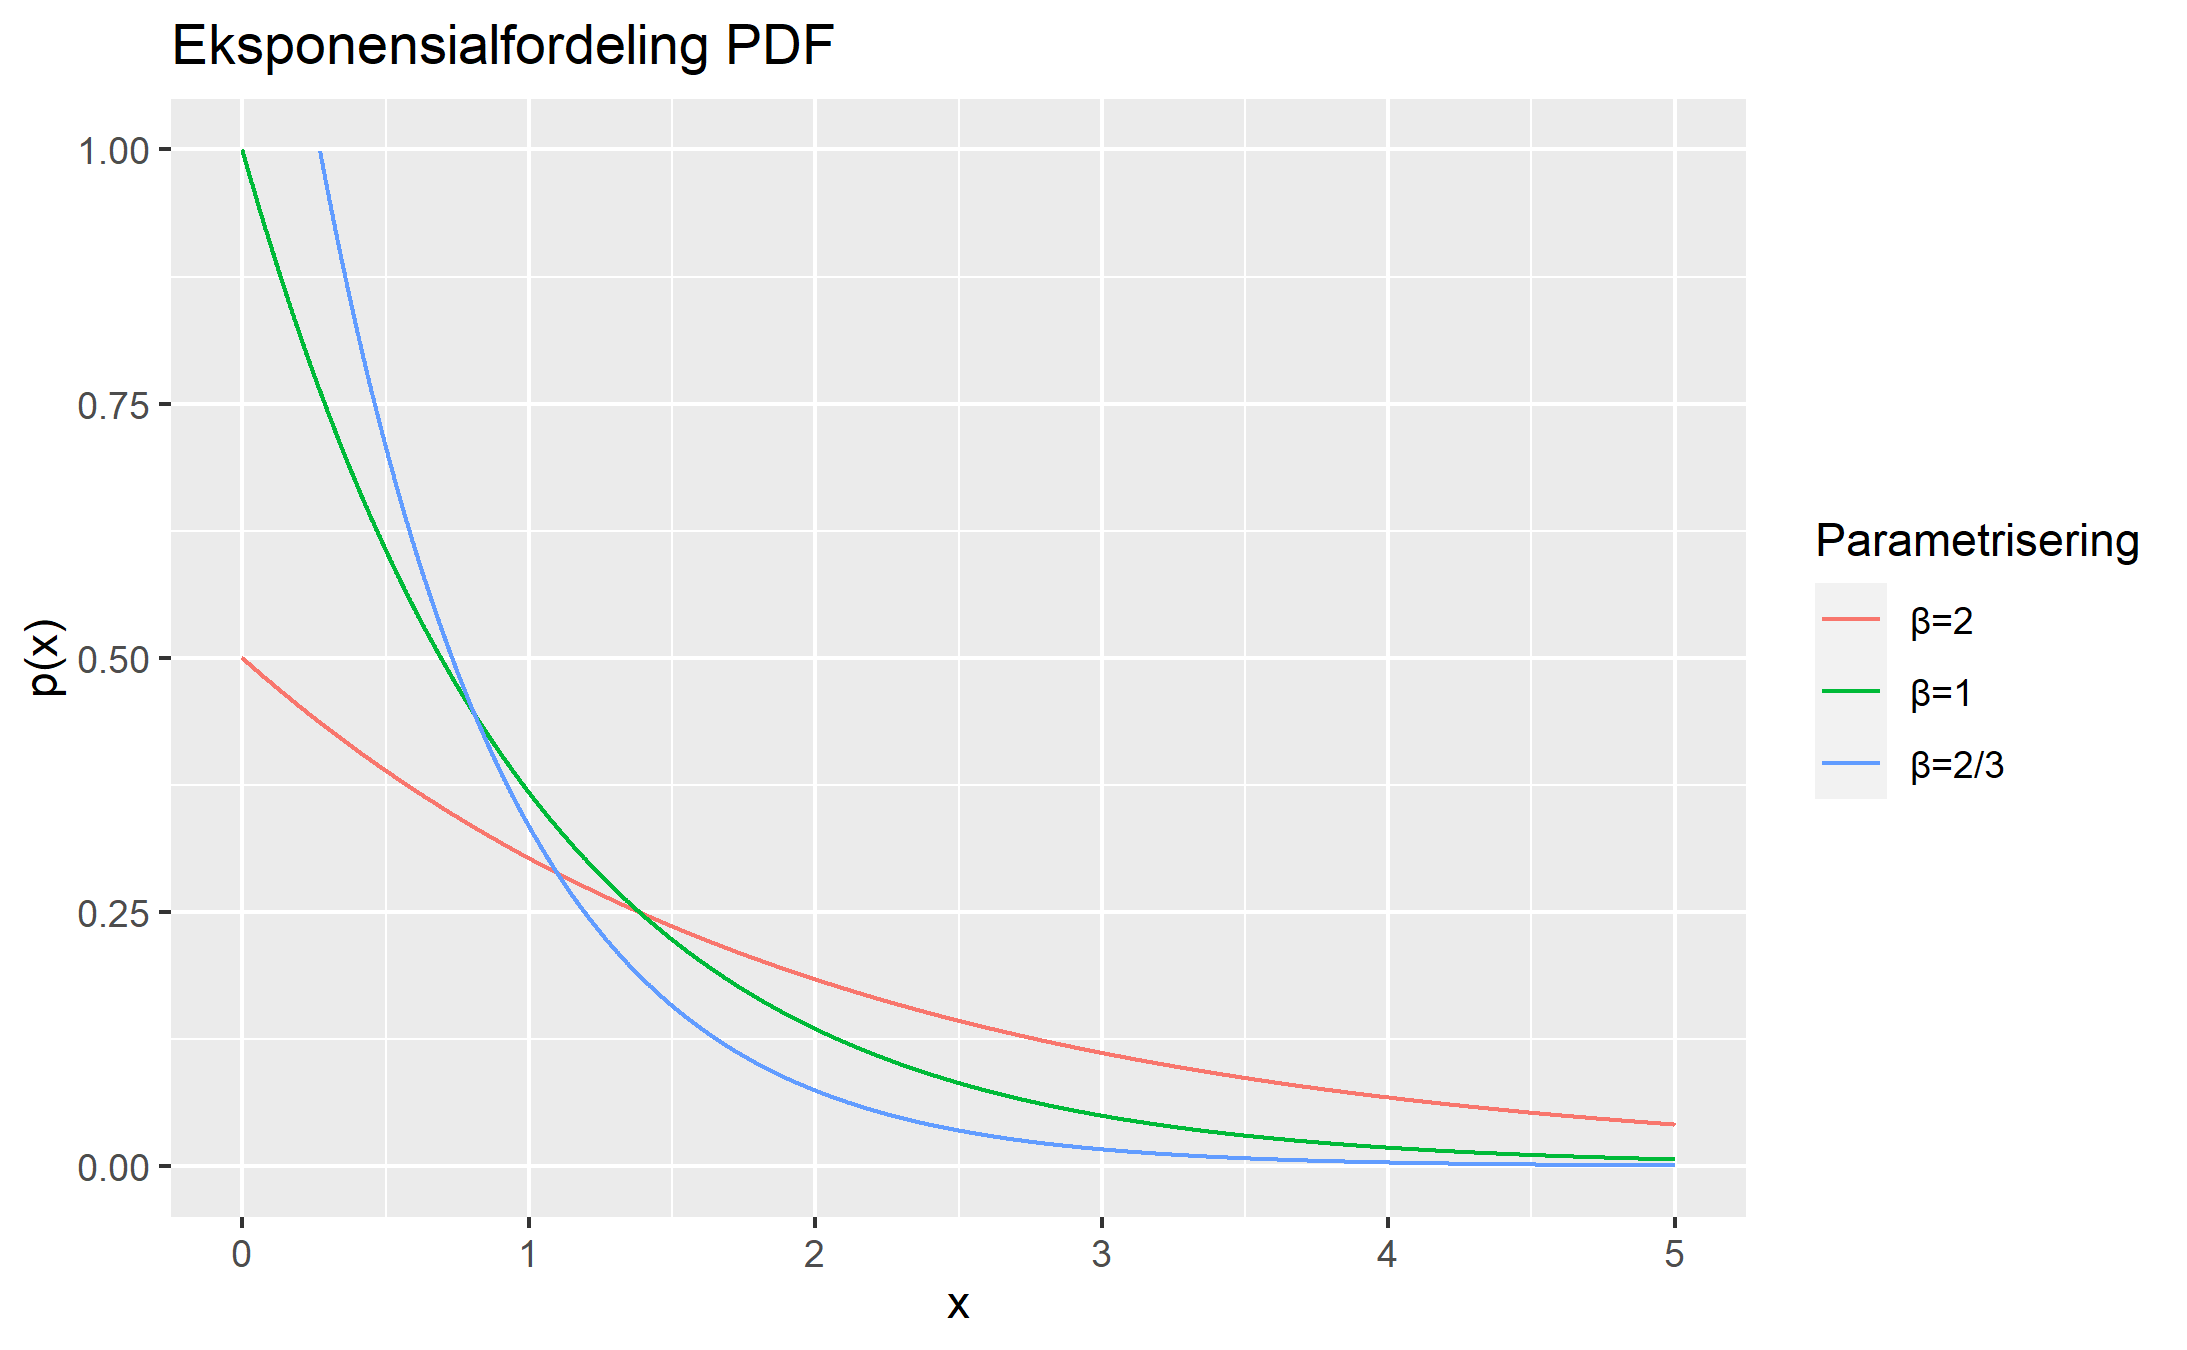
\includegraphics[width=\textwidth]{bilete/eksppdf.png}
  \end{minipage}
  \hfill
  \begin{minipage}[b]{0.49\textwidth}
    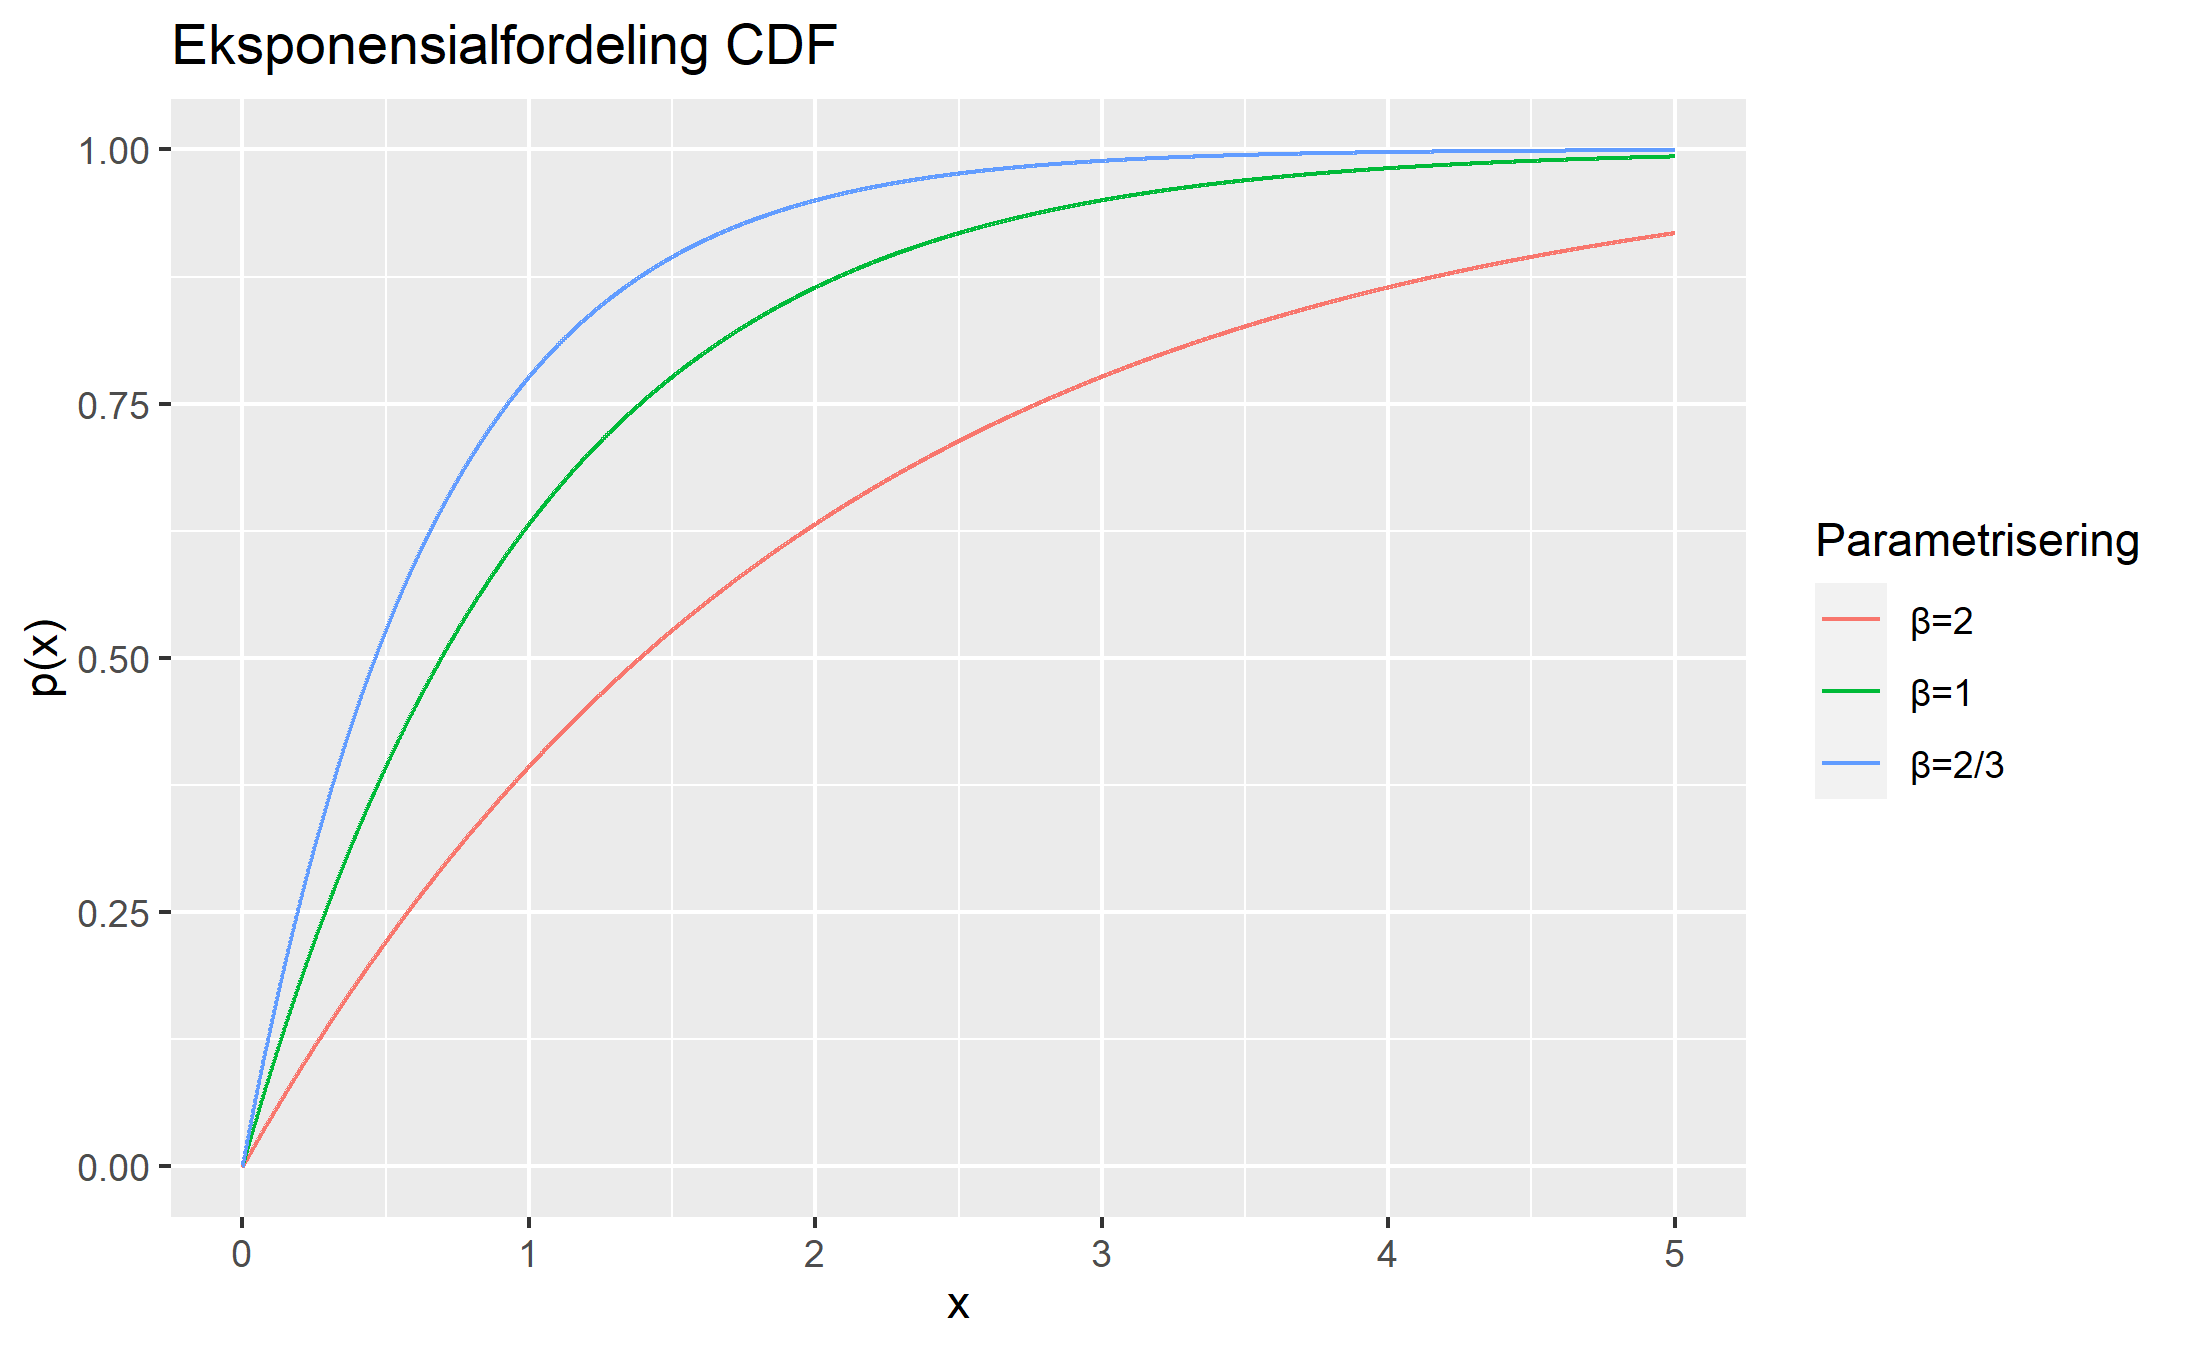
\includegraphics[width=\textwidth]{bilete/ekspcdf.png}
  \end{minipage}
\end{figure}

\subsubsection{Skalaparametrisering}\label{eksp:skala}
\begin{equation}
    f(x; \beta) = \frac{1}{\beta} e^{-\frac{x}{\beta}},  \quad  x \geq 0
\end{equation}

\begin{equation}
    F(x; \beta) = \int_{0}^x f(t) dt = 1 - e^{-\frac{x}{\beta}}
\end{equation}

\begin{equation}
    E[X] = \int_{-\infty}^{\infty} xf(x) = \beta
\end{equation}

\begin{equation}
    Var[X] = E[X^2] - E[X]^2 = \beta^2
\end{equation}

\subsubsection{Hastigheitsparametrisering}

\begin{equation}
    f(x; \lambda) = \lambda e^{\lambda x},  \quad  x \geq 0
\end{equation}

\begin{equation}
    F(x; \lambda) = \int_{0}^x f(t) dt = 1 - e^{- \lambda x}
\end{equation}

\begin{equation}
    E[X] = \int_{-\infty}^{\infty} xf(x) = \frac{1}{\lambda}
\end{equation}

\begin{equation}
    Var[X] = E[X^2] - E[X]^2 = \frac{1}{\lambda^2}
\end{equation}

\subsubsection{Eksponensialfordelingen og minnelausheit} \label{memless}
Eksponensialfordelinga blir ofte kalla for minnelaus. \cite{wiki:memless} Denne eigenskapen kan bli synt slik med følgande eksempel. Sjå føre deg at du har ei lyspære som har lyst i $300$ timar. Kva er sannsynlegheita for at den vil lyse i $500$ timar til? Om me lar $X$ være den stokastiske variabelen $X = \text{Levetid til ei lyspære i antal timar}$ så vil spørsmålet om levetid matematisk kunne formulerast slik (vha Bayes Teorem \cite{wiki:bayes}):

\begin{equation}
    P(X > 500 + 300 | X > 300) = \frac{P(X > 800 \cap X > 300)}{P(x > 300)} = \frac{P(X > 800)}{P(X > 300)} 
\end{equation}

Ved $P(X > x) = 1 - P(X \leq x) = 1 - (1 - e^\frac{-x}{\beta}) = e^\frac{-x}{\beta}$ får vi at

\begin{equation}
    \frac{P(X > 800)}{P(X > 300)} = \frac{e^\frac{-800}{\beta}}{e^\frac{-300}{\beta}} = e^\frac{-500}{\beta} = P(X > 500)
\end{equation}

Dette gir oss formelen

\begin{equation}
    P(X > t + s | X > s) = P(X > t)
\end{equation}

Dette kan tolkast som at systemet ikkje blir betre eller dårlegare over tid, at lyspæra er like god etter 300 timar som den var da den var ny og at sannsynet for at den ryk i framtida er uavhengig av kor lenge den har lyst frå før. Eksponensialfordelinga er den einaste kontinuerlige sannsynlegheitsfordelinga med denne eigenskapen. Den andre er geometrisk fordeling. 

\subsubsection{NB: Vanleg misforståing}
$P(X > 40 | X > 30) = P(X > 10)$ er korrekt bruk av formelen og \textbf{ikkje}
$P(X > 40 | X > 30) = P(X > 40)$. 

\subsection{\texorpdfstring{$\chi^2$}{chi}-fordelinga}
\begin{figure}[H]
  \centering
  \begin{minipage}[b]{0.49\textwidth}
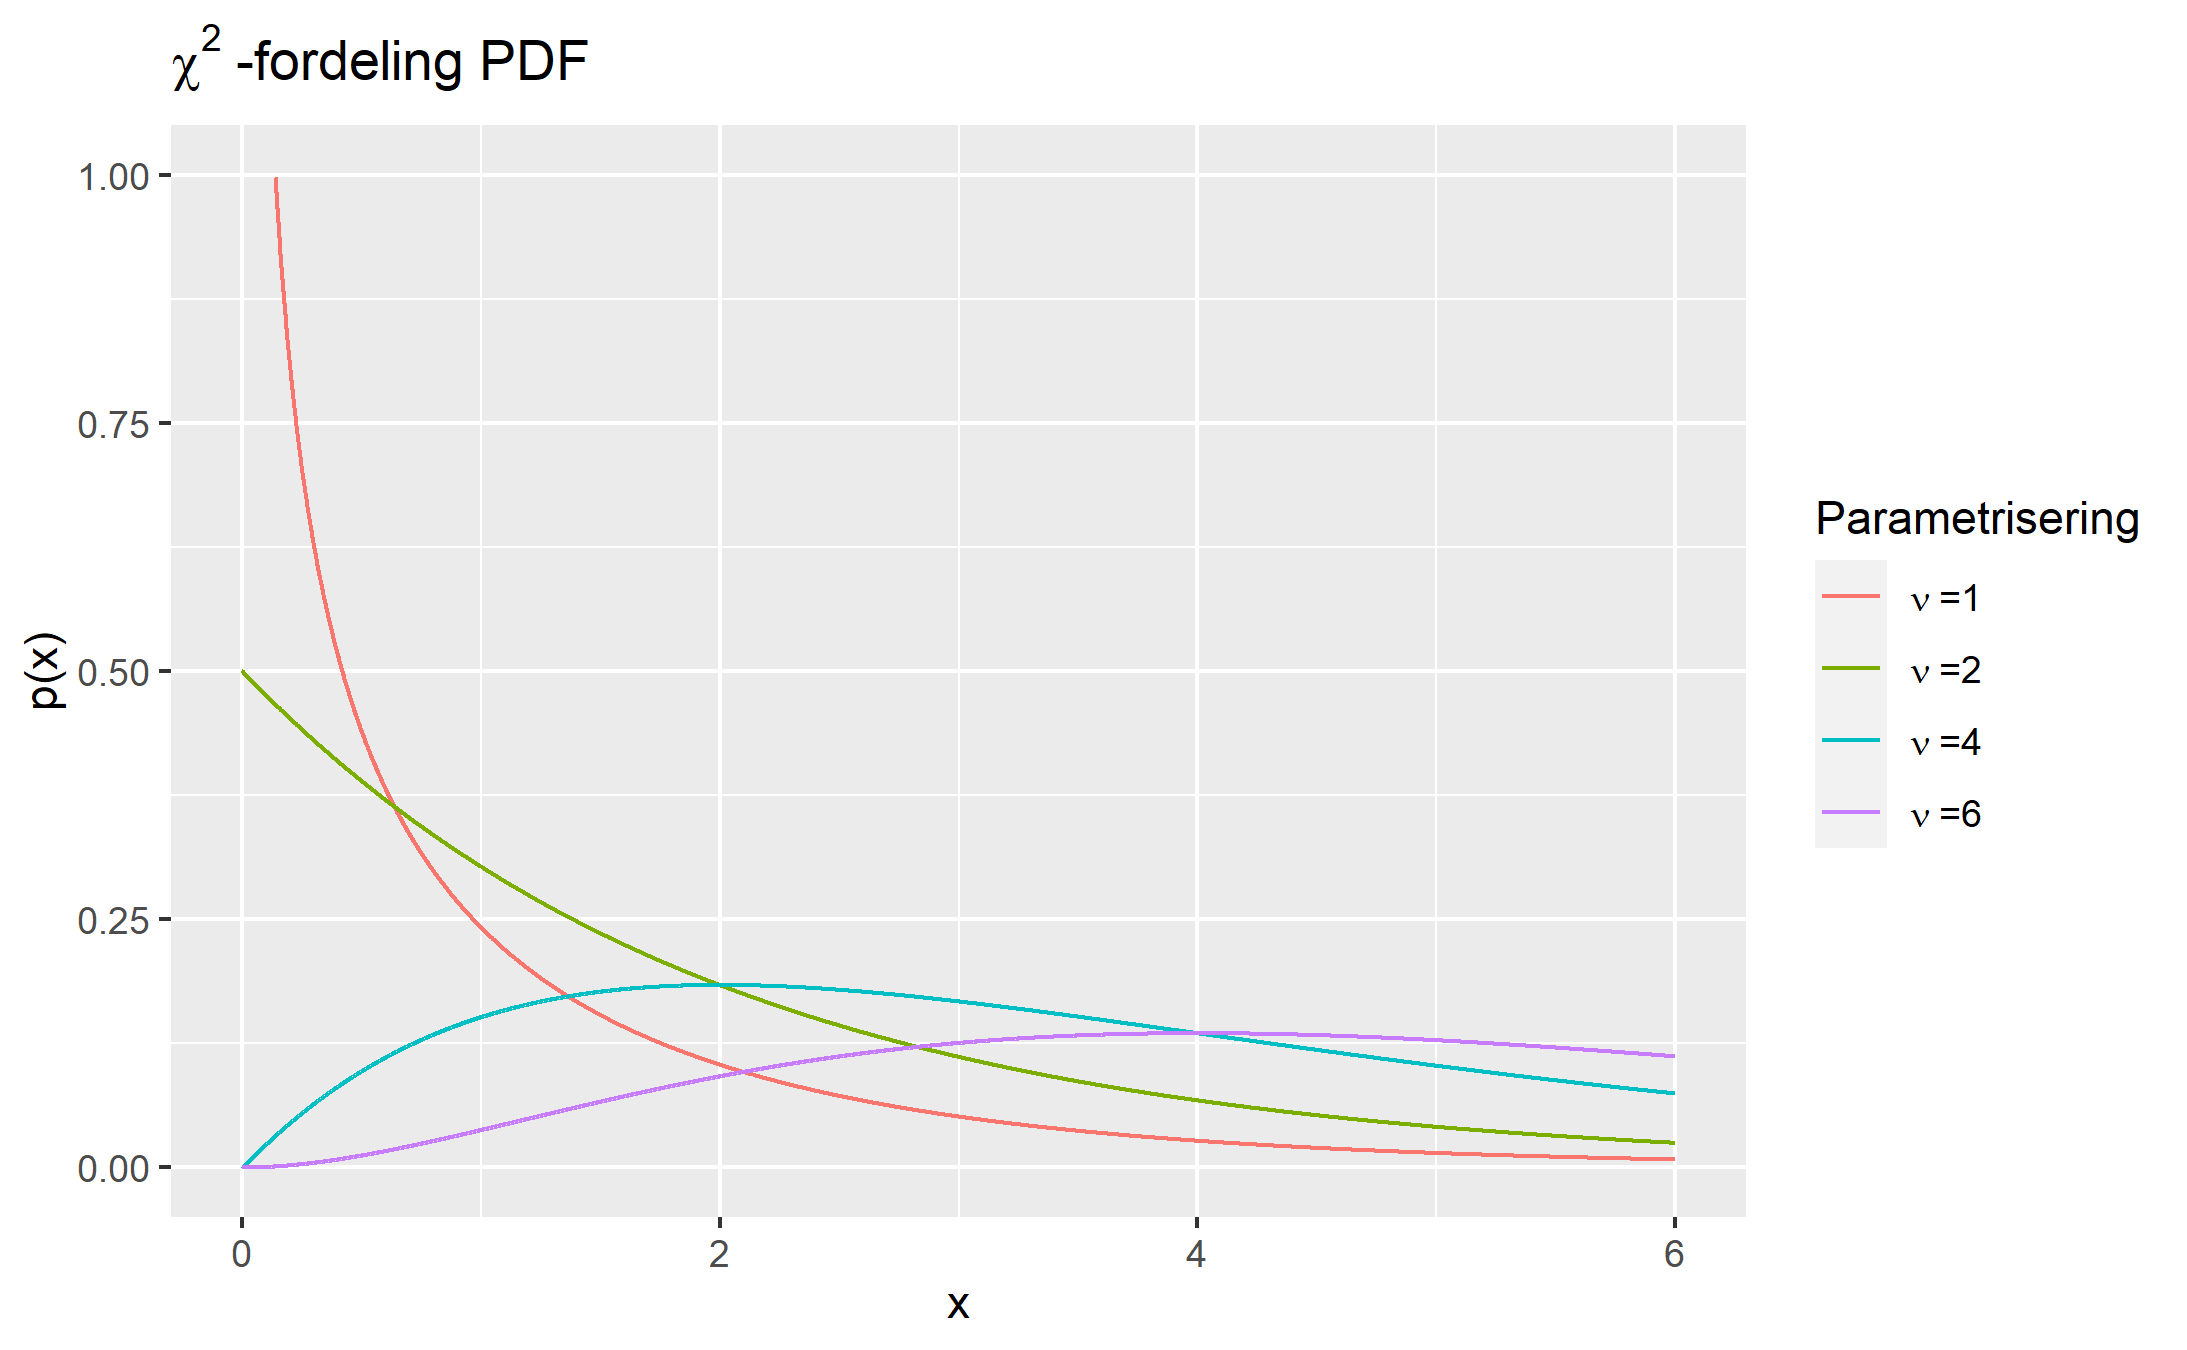
\includegraphics[width=\textwidth]{bilete/chisqpdf.png}
  \end{minipage}
  \hfill
  \begin{minipage}[b]{0.49\textwidth}
    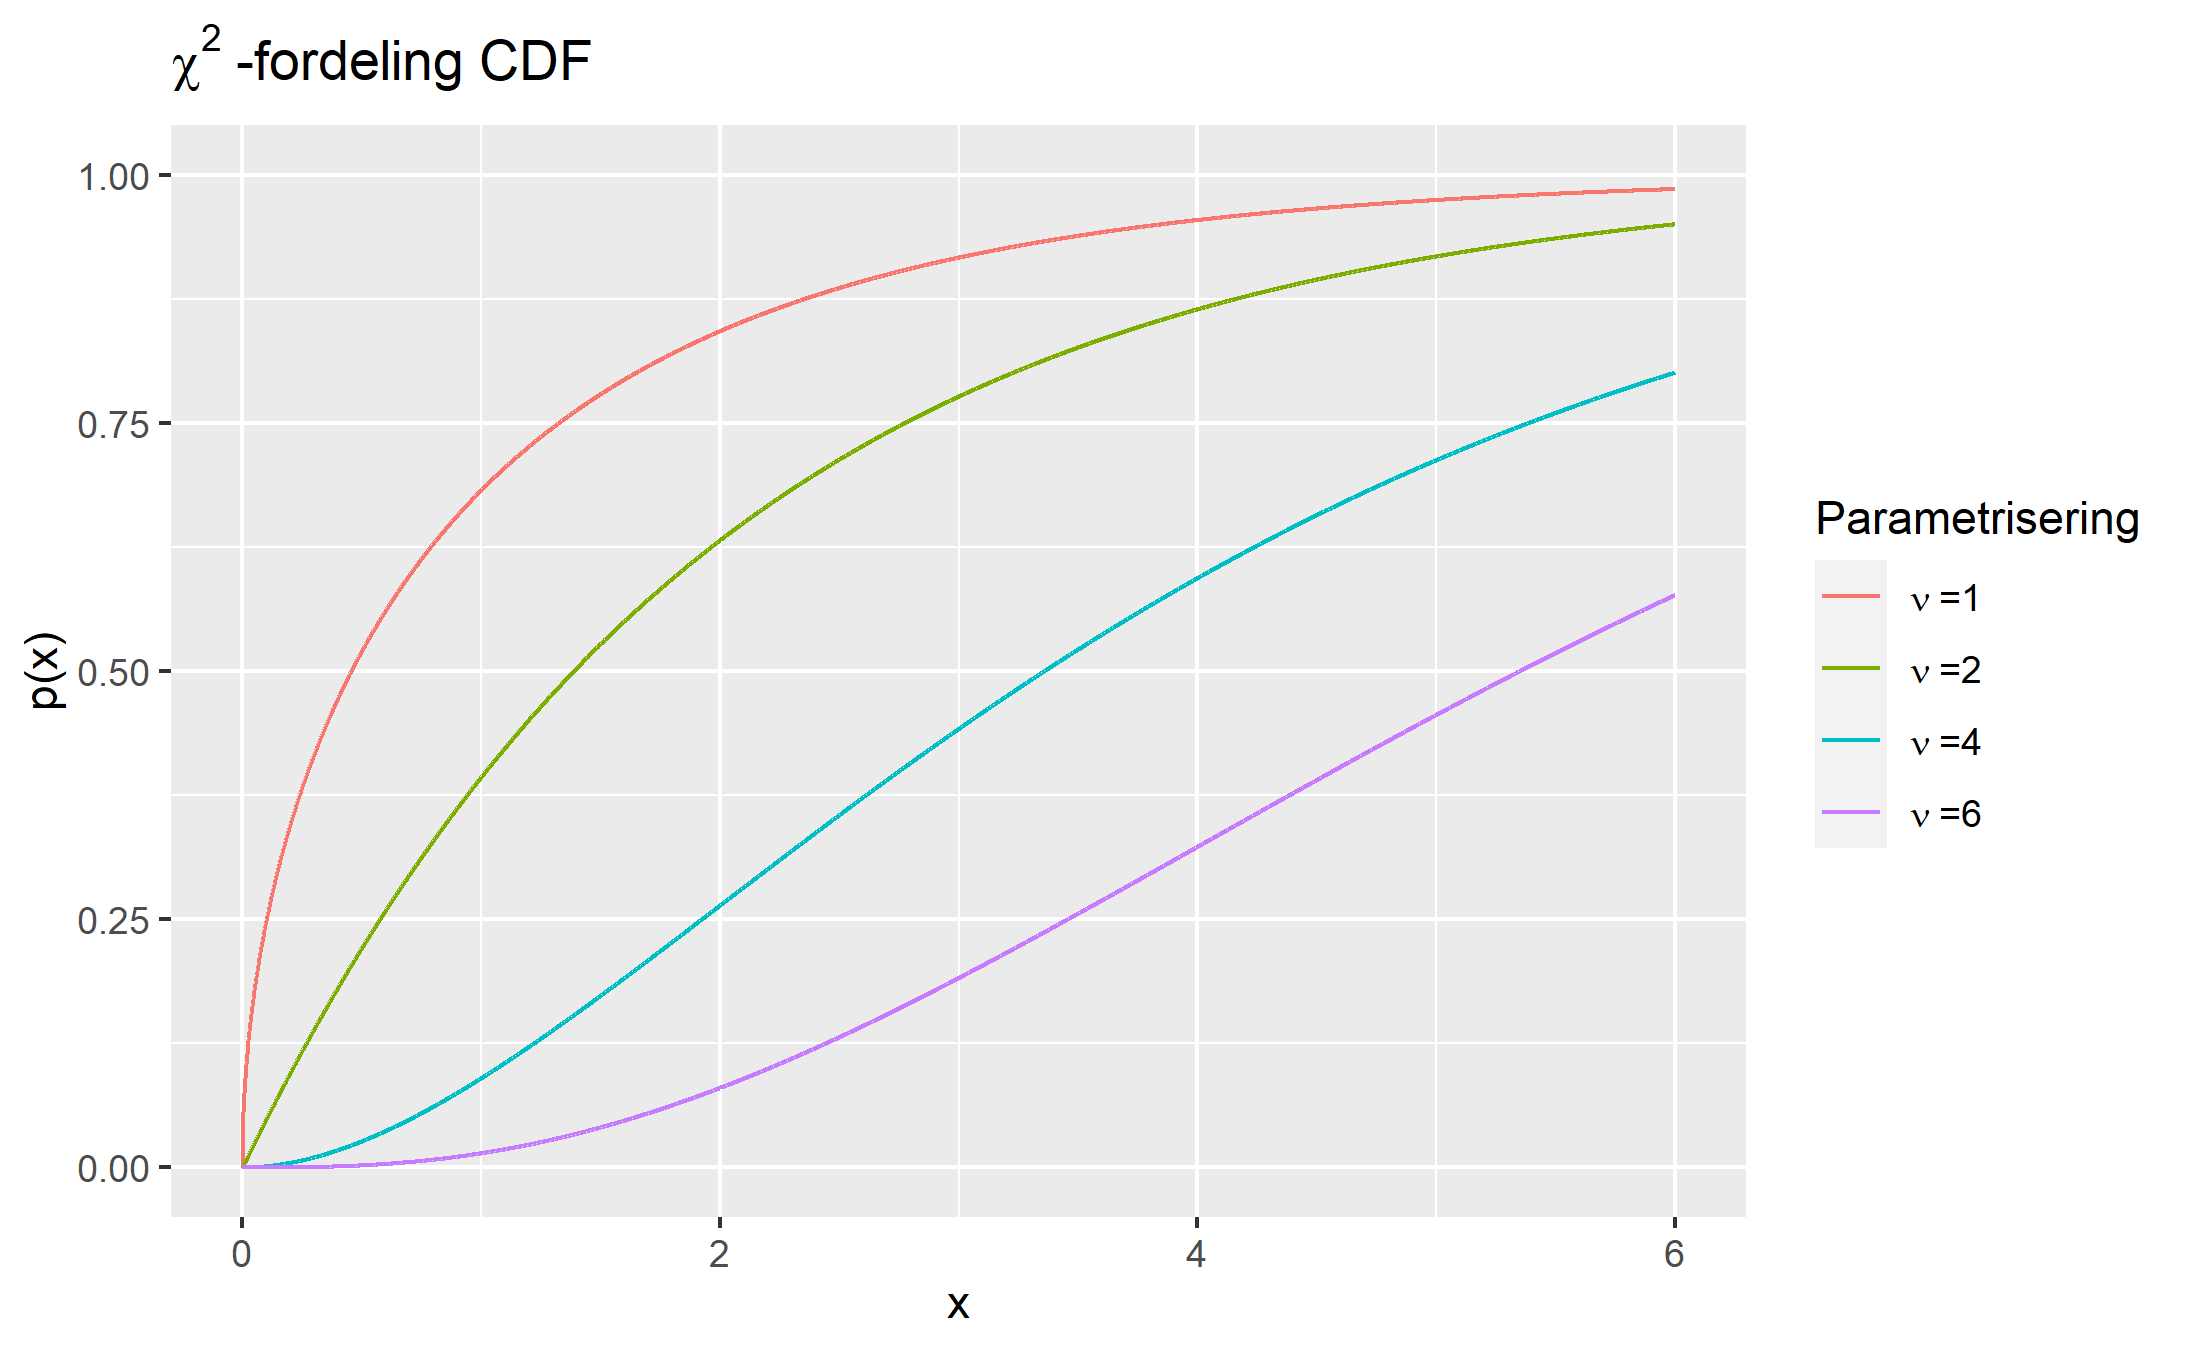
\includegraphics[width=\textwidth]{bilete/chisqcdf.png}
  \end{minipage}
\end{figure}

$\chi^2$-fordelinga er eit viktig spesialtilfelle av gammafordelinga med parameter $\alpha = \frac{\nu}{2}$ og $\beta=2$. $\chi^2$-fordelinga har kun ein parameter $\nu$ som er friheitsgrad\ref{chap:friheitsgrad}. Denne fordelinga er ein viktig fordeling med anvendingar i hypotesetestar og estimering. 

Kvifor $\chi^2$-fordelinga er nytta til hypotesetestar er langt utanfor pensum i faget. Kort oppsummert kan det forklarast ved at $\chi^2$-fordelinga er relatert til normalfordelingen gjennom at om ein tar ein fordeling $Z \sim N(0,1)$ så er $Z^2 \sim \chi^2$ fordelt med $\nu = 1$ og på grunn av sentralgrenseteoremet\ref{chap:sentralgrense} vil mange fordelingar kunne estimerast med ein normalfordeling.

\begin{equation}
    f(x; \nu) = \frac{1}{2^{\nu/2}\Gamma(\nu/2)}x^{\nu/2 - 1}e^{-x/2}, \qquad x > 0
\end{equation}

\begin{equation}
    F(x; \nu) = \frac{1}{\Gamma(\nu / 2)} \gamma(\frac{\nu}{2}, \frac{x}{2}), \qquad x > 0
\end{equation}

Der $\gamma$ er den inkomplette-gammafunksjonen \cite{wiki:incomgamma} og $\Gamma$ er gammafunksjonen \cite{walpole2012probability}. Desse reknar me i praksis ut vha verktøy som R. 

\begin{equation}
    E[X] = \nu
\end{equation}

\begin{equation}
    Var[X] = E[X^2] - E[X]^2 = 2\nu
\end{equation}

\subsection{Betafordeling}
\begin{figure}[H]
  \centering
  \begin{minipage}[b]{0.49\textwidth}
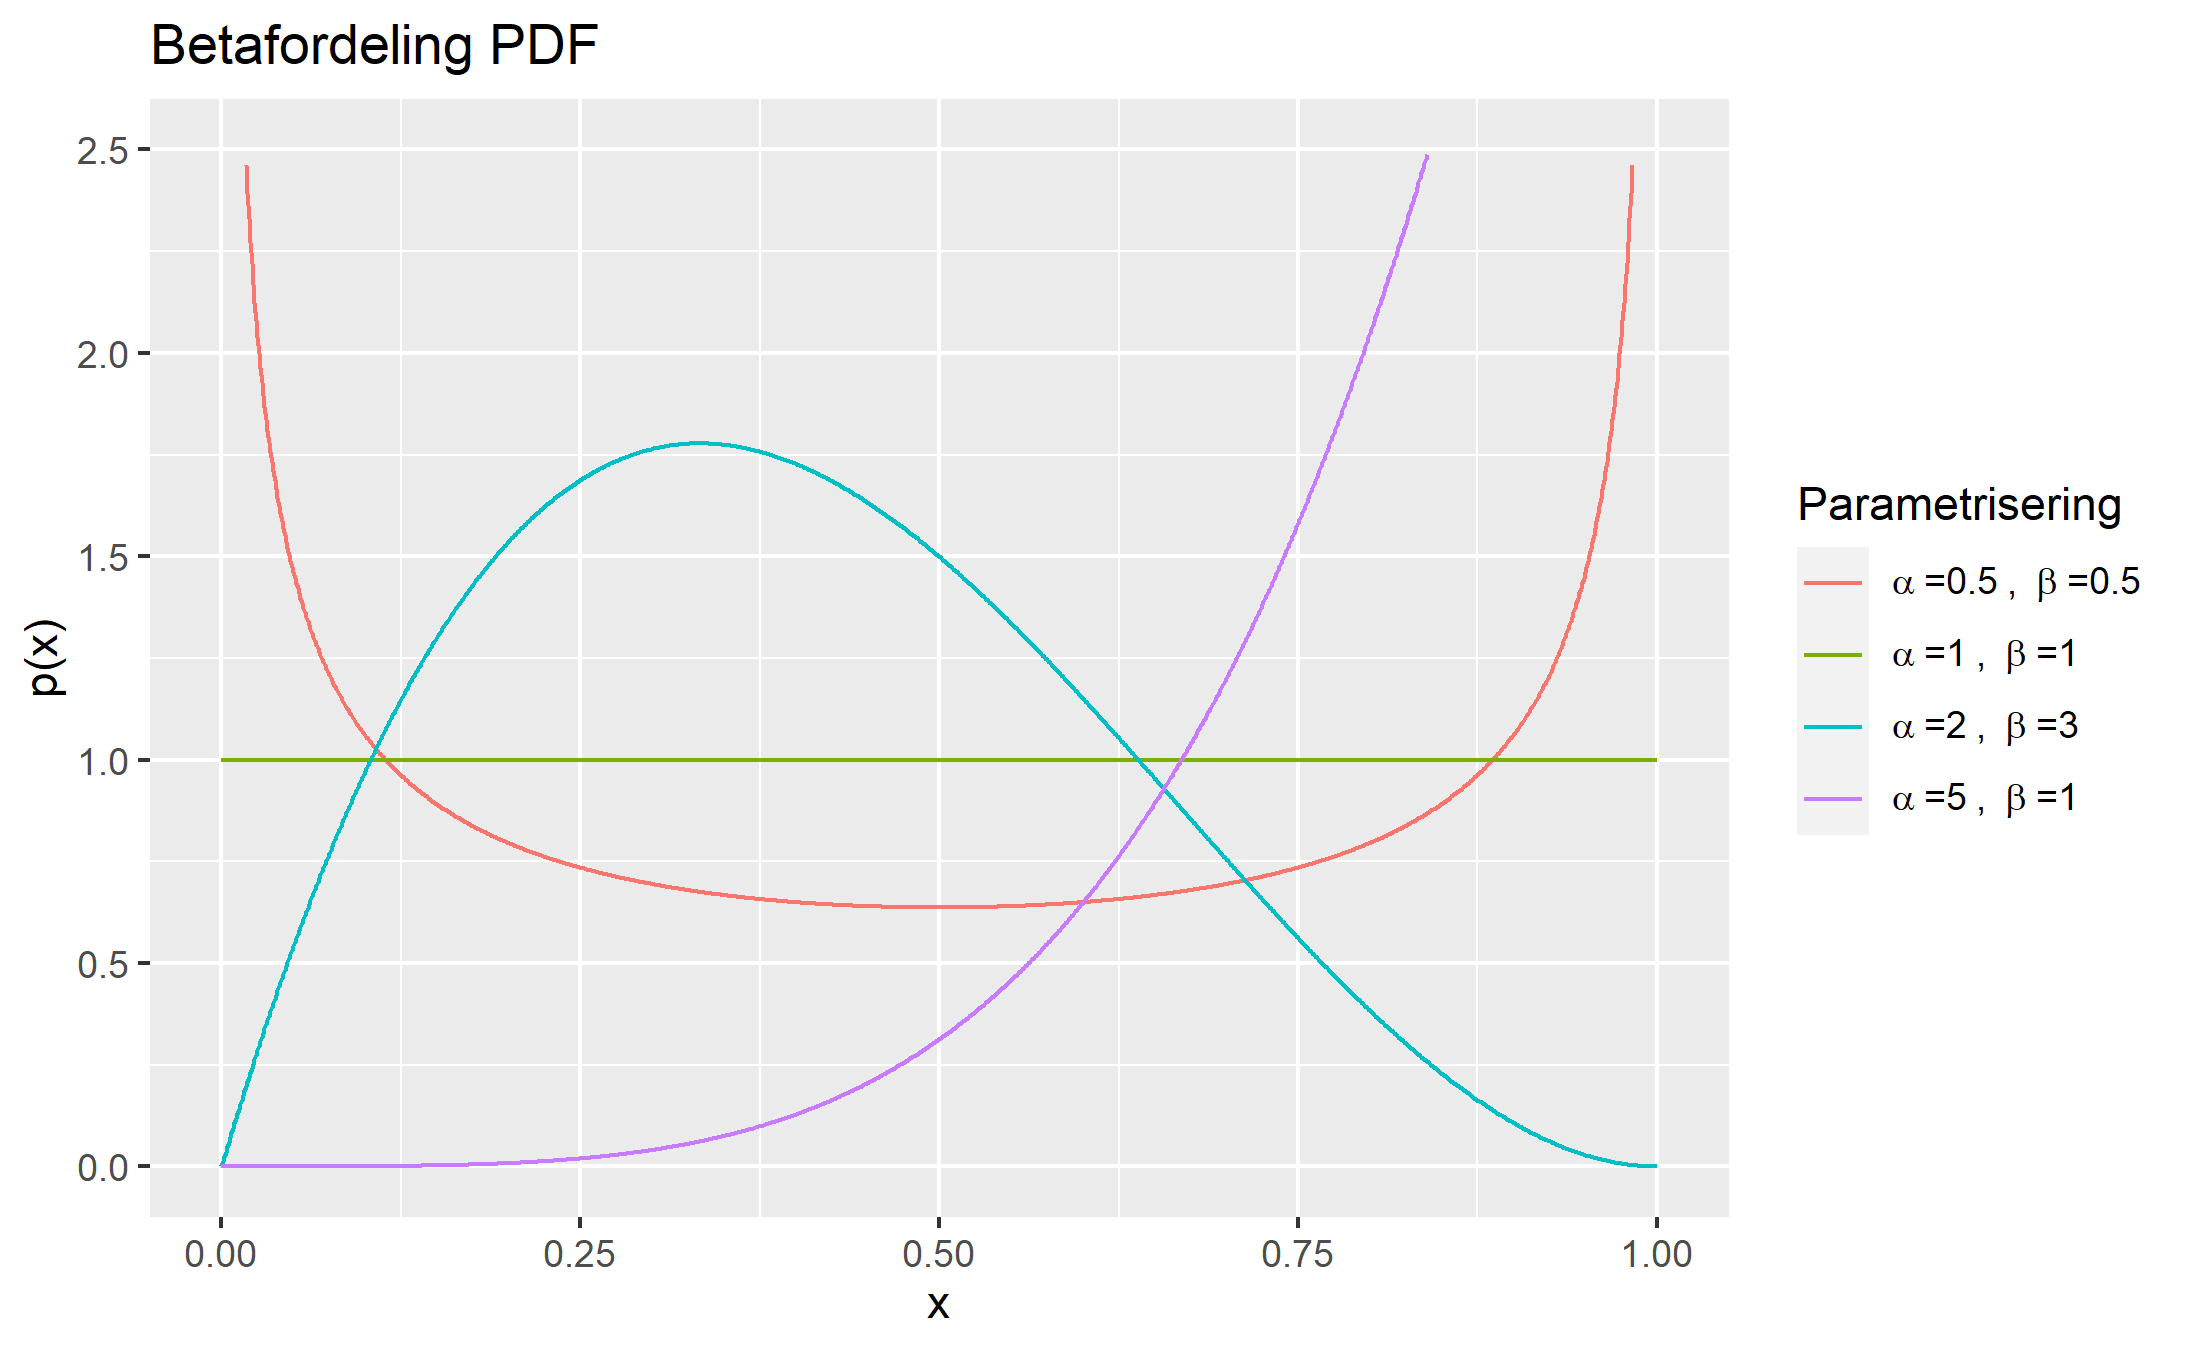
\includegraphics[width=\textwidth]{bilete/betapdf.png}
  \end{minipage}
  \hfill
  \begin{minipage}[b]{0.49\textwidth}
    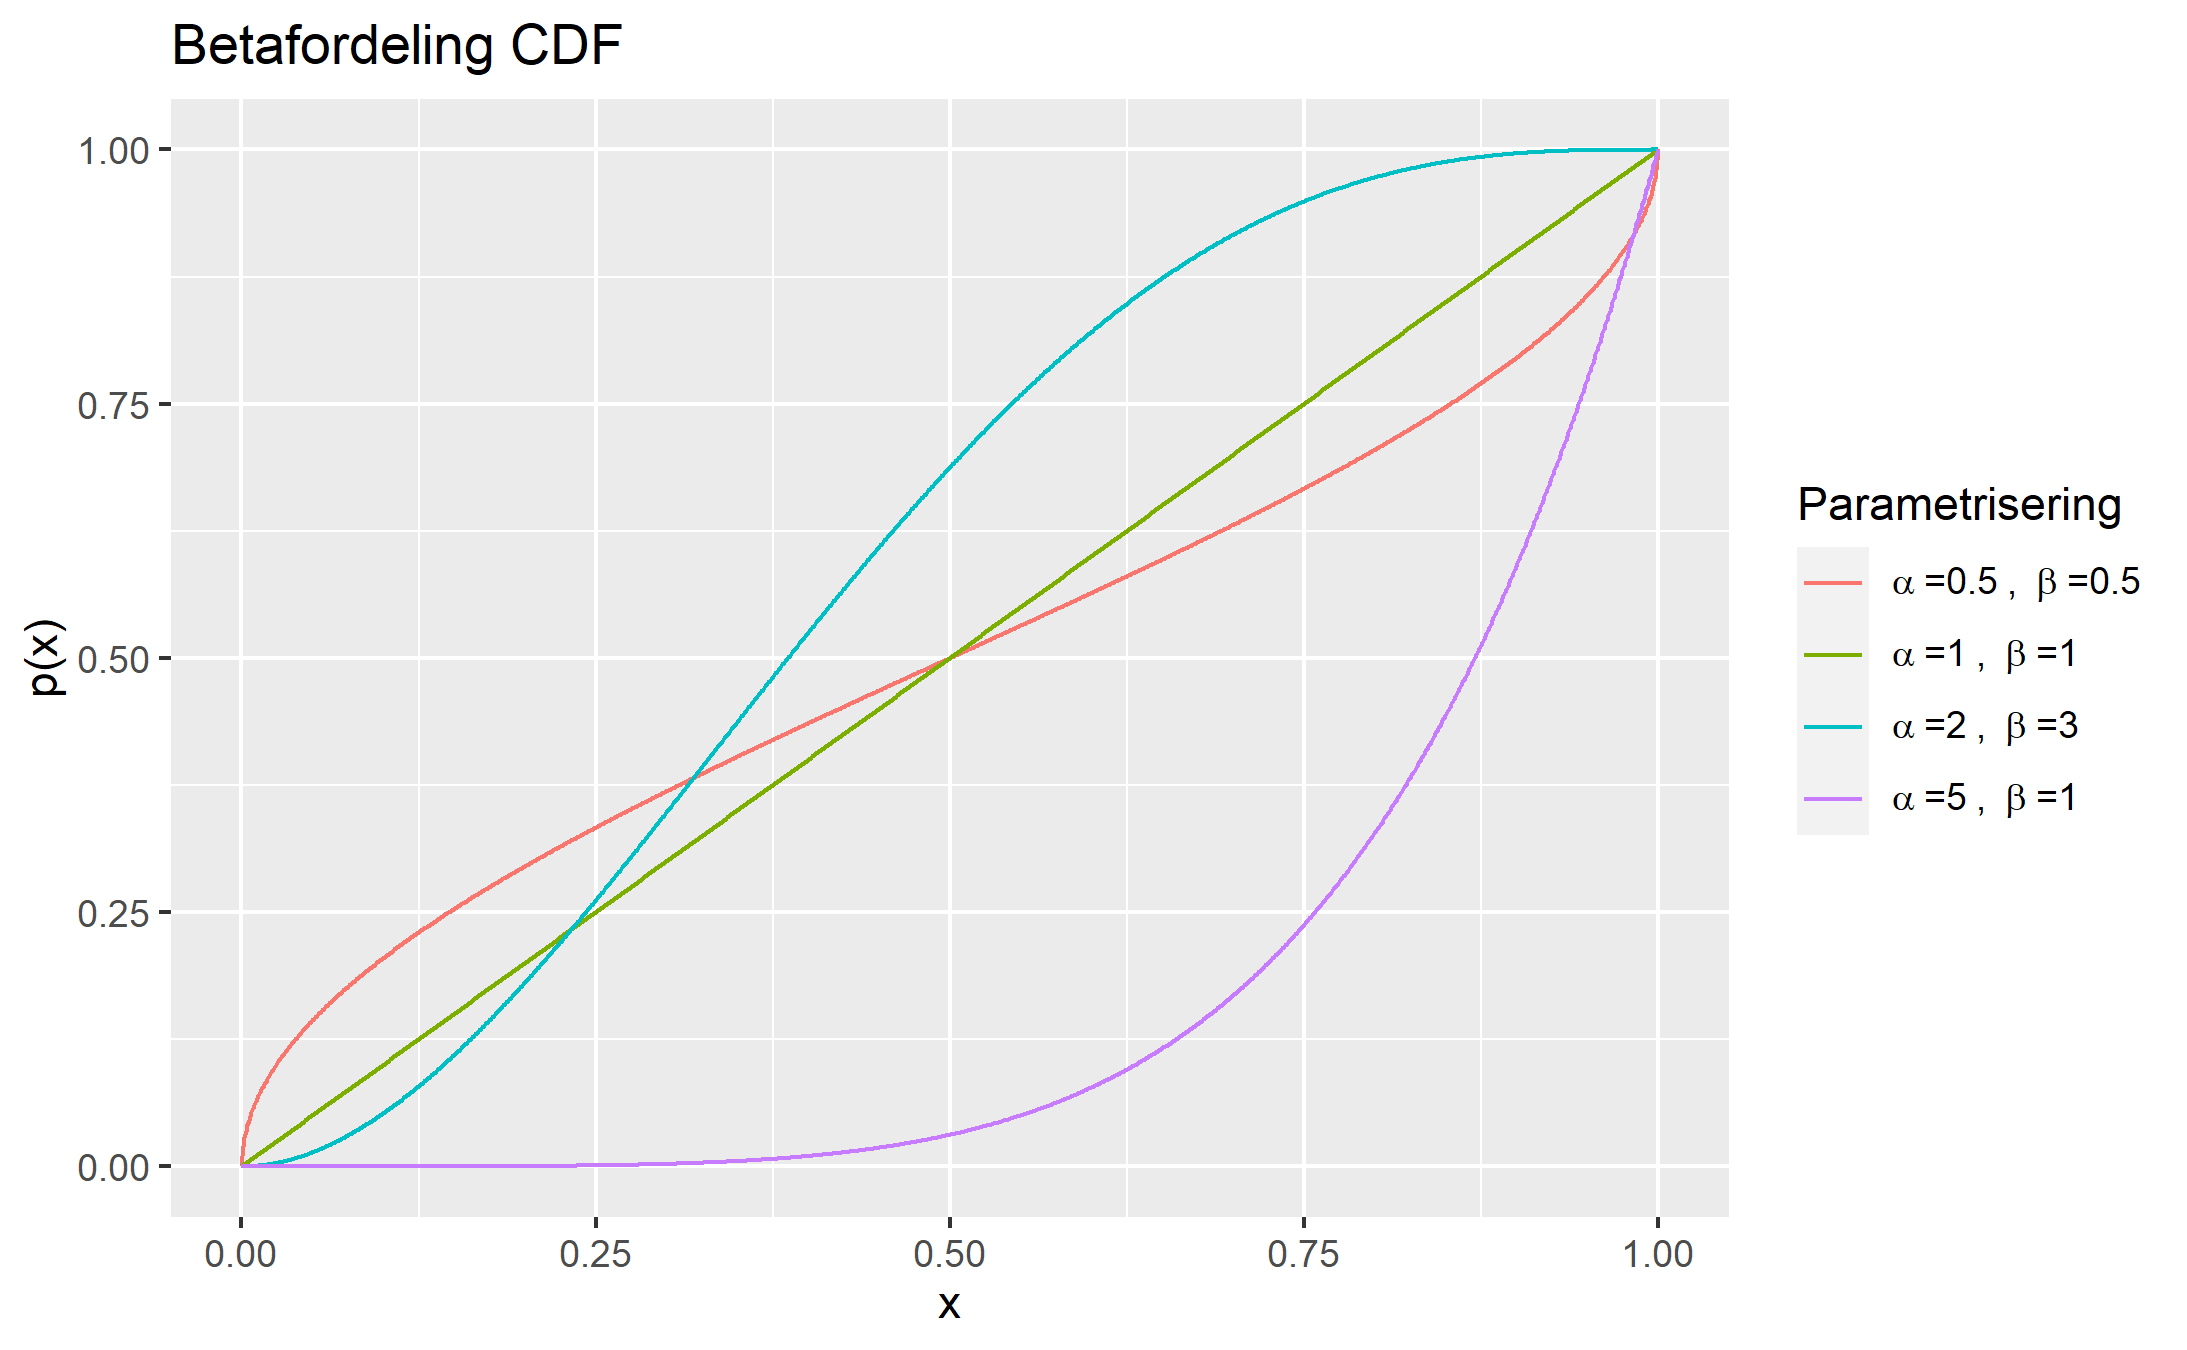
\includegraphics[width=\textwidth]{bilete/betacdf.png}
  \end{minipage}
\end{figure}

Ein utvidelse av den uniforme fordelinga er betafordelinga. Den har to formparameter $\alpha$ og $\beta$ og når begge desse er lik $1$ har du den standard uniforme fordelinga på intervallet $[0, 1]$. Betafordelinger blir ofte brukt som ein konjugert à priori-fordeling i bayesiansk slutningsteori. Dette gjelder for bernoulli, binomsik, negativ binomsik og geometrisk fordeling.

\begin{equation}
    f(x; \alpha, \beta) = 
    \begin{cases}
        \frac{1}{B(\alpha, \beta)}x^{\alpha - 1}(1 - x)^{\beta - 1} & 0 < x < 1 \\
        0 & \text{Ellers}
    \end{cases}
\end{equation}

der \textbf{Beta funksjonen} er definert som

\begin{equation*}
    B(\alpha, \beta) = \int_0^1 x^{\alpha - 1}(1 - x)^{\beta - 1} \,dx = \frac{\Gamma(\alpha)\Gamma(\beta)}{\Gamma(\alpha + \beta)}, \qquad \text{for } \alpha, \beta > 0
\end{equation*}

der $\Gamma$ er gammafunksjonen \cite{walpole2012probability}. 

\begin{equation}
    F(x; \alpha, \beta) = I_x(\alpha, \beta) = \frac{B(x; \alpha, \beta)}{B(\alpha, \beta)}
\end{equation}

Der $I_x$ er den regulariserte ukomplette beta funksjonen og vi har den \textbf{ukomplette beta funksjonen:}

\begin{equation*}
    B(x; \alpha, \beta) = \int_0^x t^{\alpha-1}(1 - t)^{\beta - 1} \, dt
\end{equation*}

\begin{equation}
    E[X] = \frac{\alpha}{\alpha + \beta}, \qquad \text{Var}(X) = \frac{\alpha\beta}{(\alpha + \beta)^2(\alpha + \beta + 1)}
\end{equation}

\subsection{Lognormalfordeling}
\begin{figure}[H]
  \centering
  \begin{minipage}[b]{0.49\textwidth}
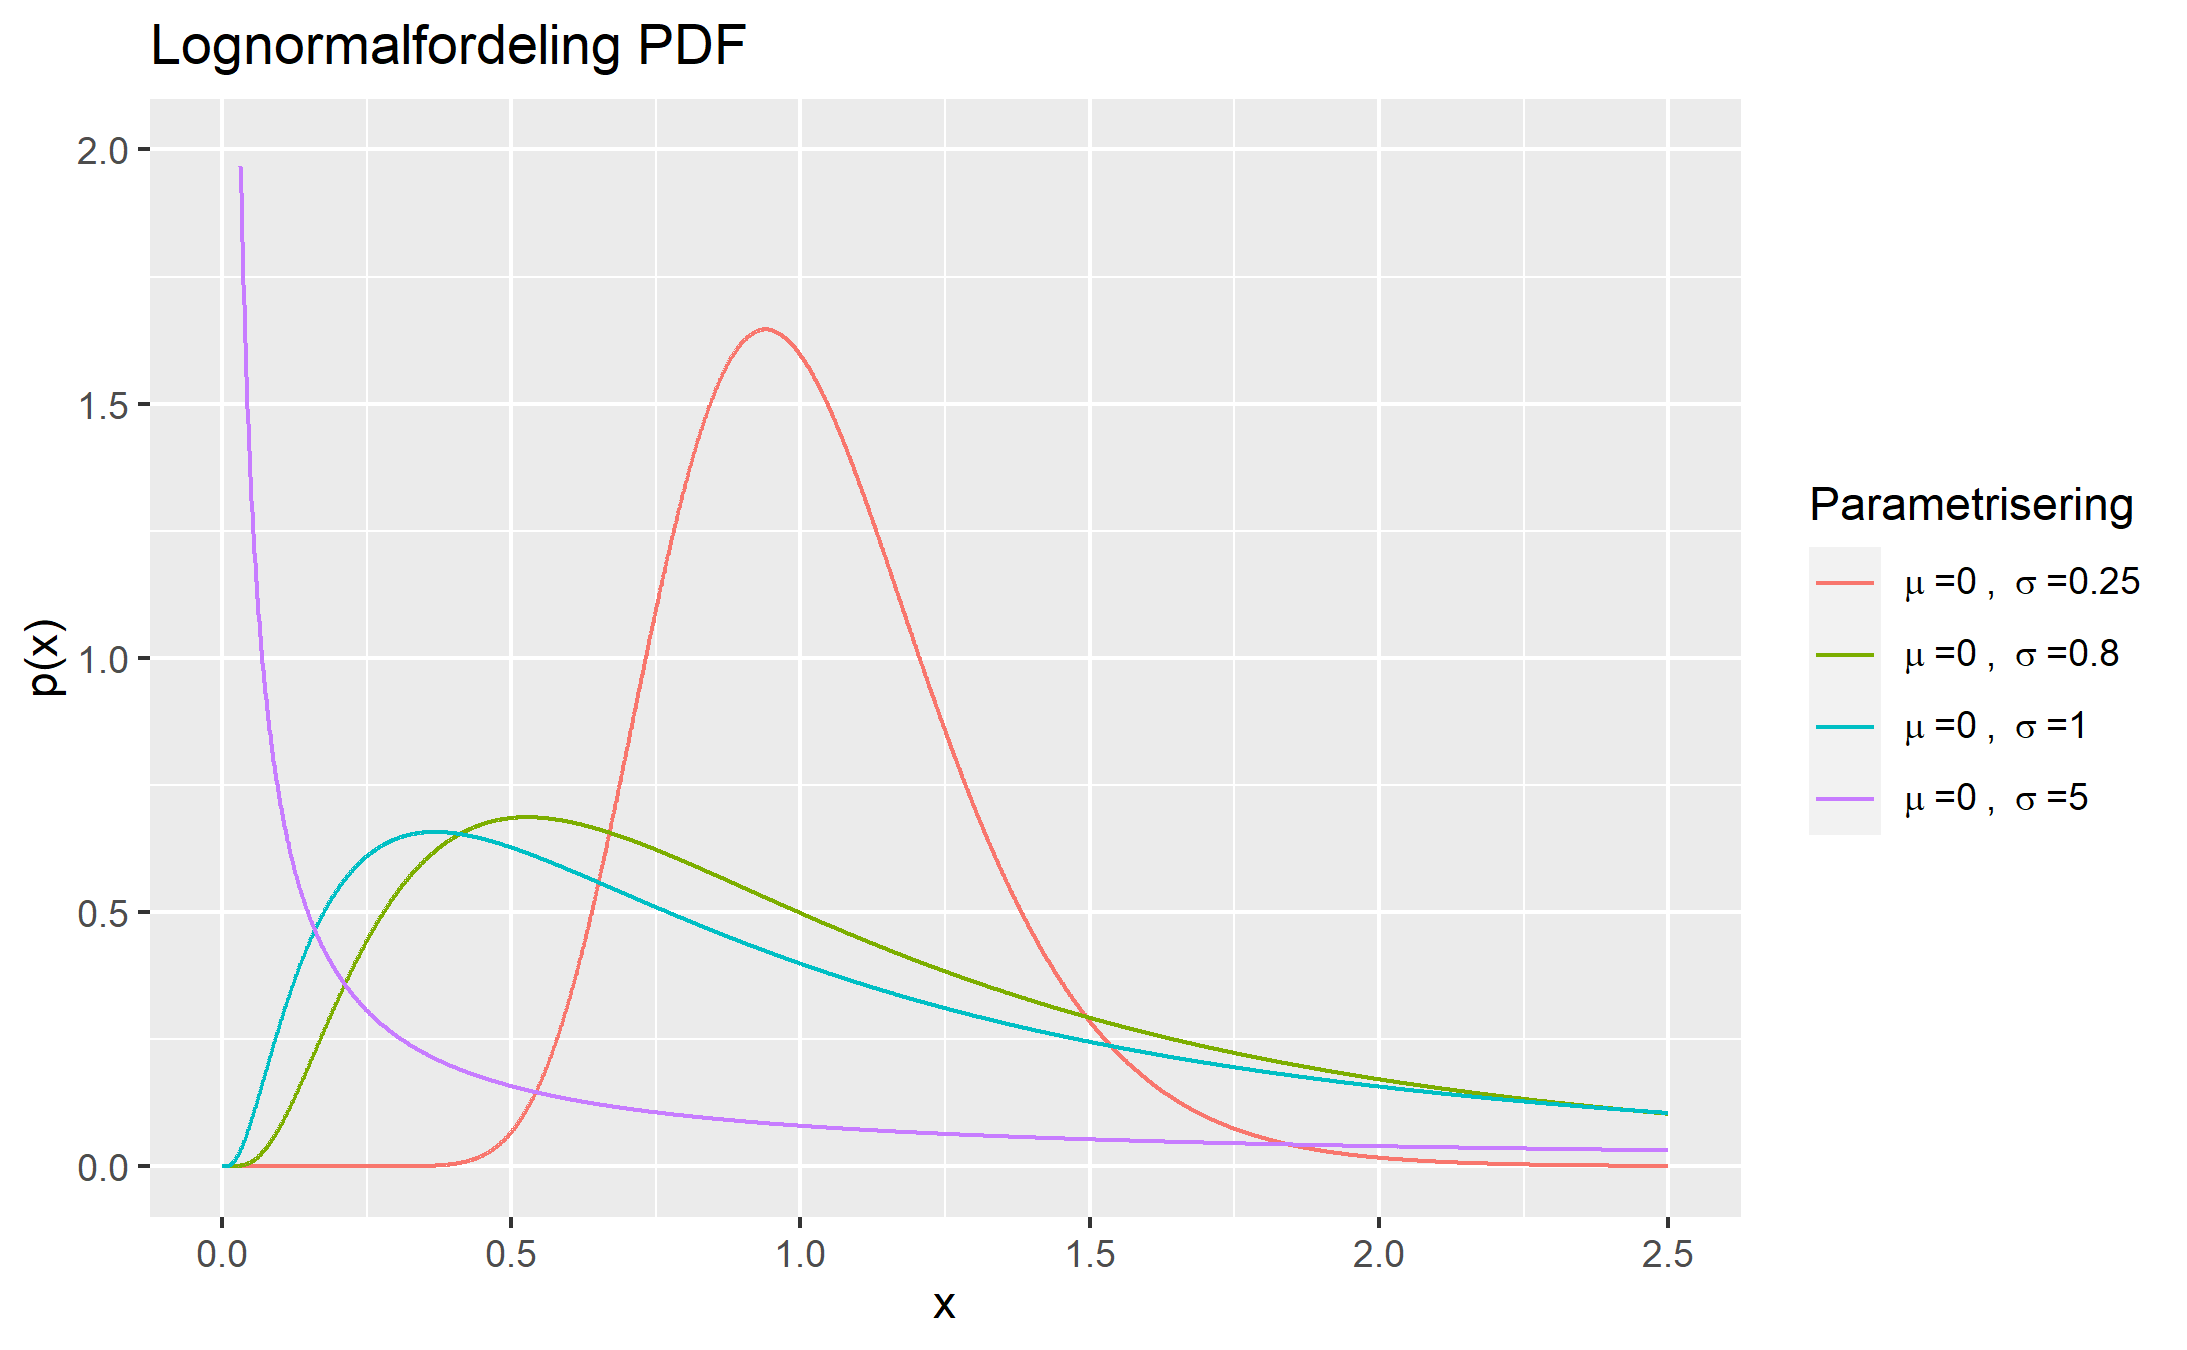
\includegraphics[width=\textwidth]{bilete/lognormalpdf.png}
  \end{minipage}
  \hfill
  \begin{minipage}[b]{0.49\textwidth}
    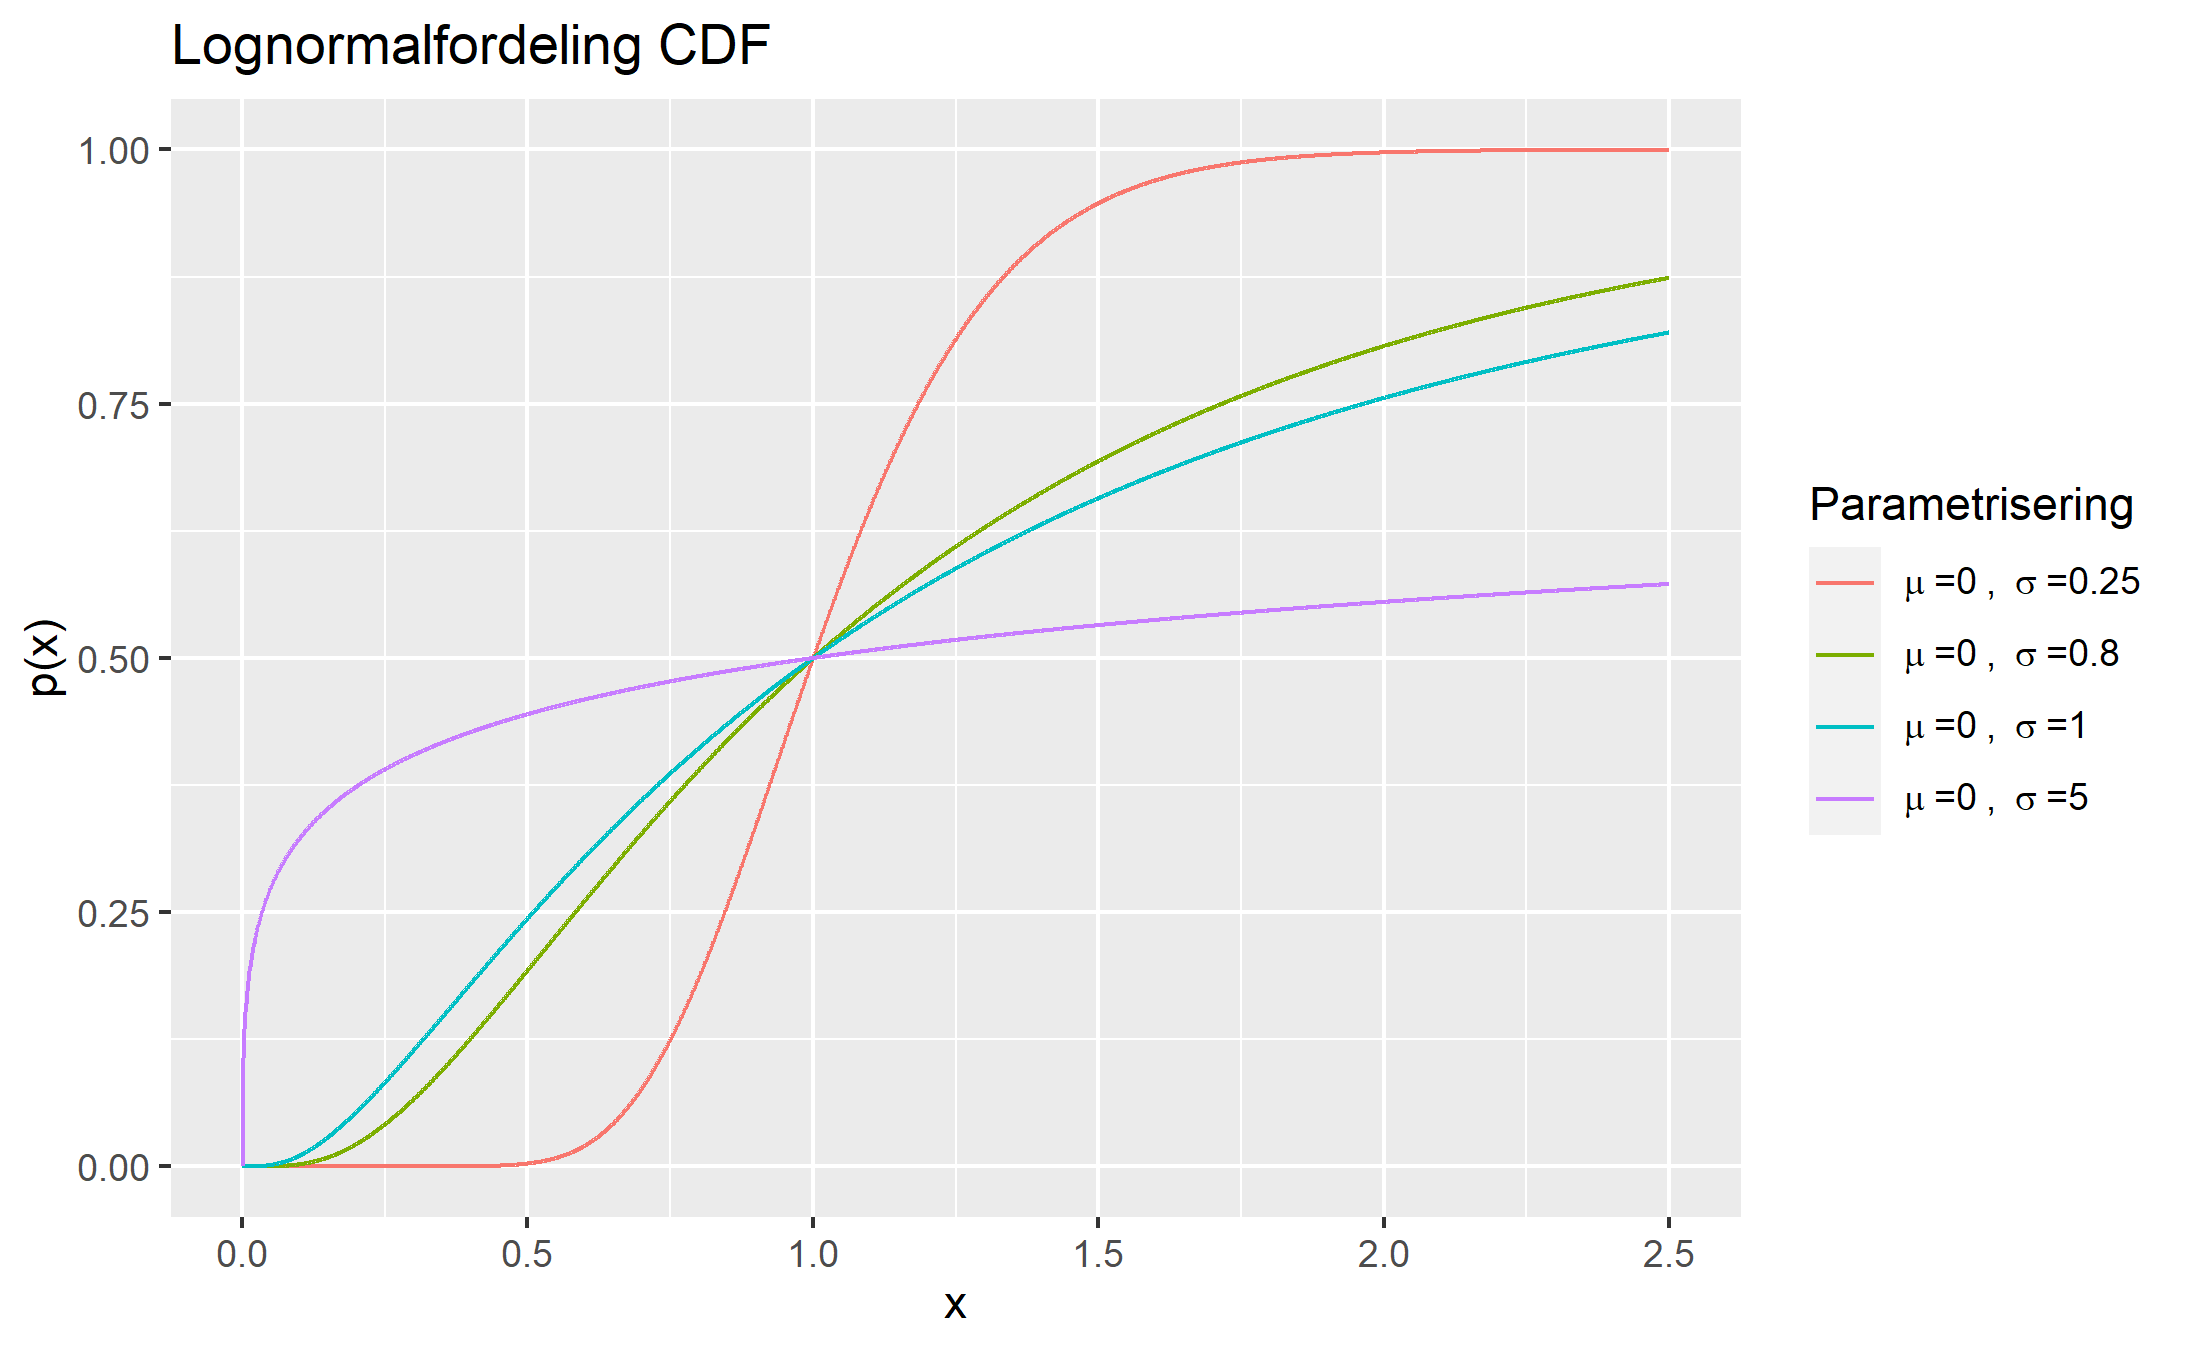
\includegraphics[width=\textwidth]{bilete/lognormalcdf.png}
  \end{minipage}
\end{figure}

Lognormalfordeling er ein fordeling med mange bruksområde. Matematisk definerer vi den ved at gitt at ein variabel $X$ er lognormalfordelt så vil den stokastiske variabelen $Y$ vere normalfordelt når

\begin{equation}
    Y = \ln(X)
\end{equation}
 eller ein kan definere ein normalfordelt variabel $X$ og ein får då ein lognormalfordelt variabel $Y$ når \begin{equation}
     Y = \exp(X)
 \end{equation}

Intuitivt, som demonstrert i kapittelet om \textbf{sentralgrenseteoremet}\ref{chap:sentralgrense} så er  summen/differansen/gjennomsnittet av fleire identiske variablar $X$ normalfordelt. Lognormalfordelinga får ein når ein har gjentatt multiplikasjon av ein variabel. Det er derfor ein mykje brukt fordeling for å modellere fenomen der gjentatt multiplikasjon dukker opp (som f.eks daglig prosentvekst).

\begin{equation}
    f(x; \mu, \sigma) = \frac{1}{\sqrt{2\pi}\sigma x}e^{-\frac{1}{2\sigma^2}[ \ln(x) - \mu]}, \qquad x > 0
\end{equation}

\begin{equation}
    F(x; \mu, \sigma) = P(X \leq x) = \boldsymbol{\phi}\left(\frac{\ln(x) - \mu}{\sigma}\right)
\end{equation}

Der $\phi$ er den standard normalfordelingen. Dette er på grunn av det same problemet som er diskutert i kapittel \ref{chap:normpraksis}. Normalfordelingen er vanskeleg å integrere for deler av intervallet og i praksis benytter me oss av tabellar eller programvare som R for å rekne ut den kumulative funksjonen.

\begin{equation}
    E[X] = e^{\mu + \sigma^2/2}
\end{equation}

\begin{equation}
    Var[X] = E[X^2] - E[X]^2 = e^{2\mu + \sigma^2}(e^{\sigma^2} - 1)
\end{equation}